\documentclass[10pt,twoside]{article}

\usepackage{iftex}

\ifPDFTeX
\usepackage[utf8]{inputenc}
\usepackage[T5]{fontenc}
\usepackage[vietnamese]{babel}
\usepackage{mathptmx}
\usepackage[scaled=0.92]{helvet}
\newcommand{\arialfont}{\fontfamily{phv}\selectfont}
\else
\usepackage[vietnamese]{babel}
\usepackage{fontspec}
\defaultfontfeatures{Ligatures=TeX}

\IfFontExistsTF{Times New Roman}
{\setmainfont{Times New Roman}}
{\setmainfont{TeX Gyre Termes}}

\IfFontExistsTF{Arial}
{\setsansfont{Arial}\newfontfamily\arialfont{Arial}}
{\setsansfont{TeX Gyre Heros}\newfontfamily\arialfont{TeX Gyre Heros}}
\fi

% ------------------ Page layout theo template FAIR ------------------
\usepackage[
paperwidth=20.5cm,
paperheight=29.5cm,
top=2.2cm,
bottom=1.8cm,
left=1.8cm,
right=1.8cm,
headheight=13pt,
headsep=0.4cm,
footskip=0.8cm
]{geometry}

% ------------------ Packages ------------------
\usepackage{amsmath,amssymb}
\usepackage{graphicx}
\usepackage{array}
\usepackage{longtable}
\usepackage{caption}
\usepackage{subcaption}
\usepackage{float}
\usepackage{enumitem}
\usepackage{fancyhdr}
\usepackage{titlesec}
\usepackage{indentfirst}
\usepackage{url}
\IfFileExists{cite.sty}{\usepackage{cite}}{}

\newcommand{\fairsmallfont}{\fontsize{9pt}{11pt}\selectfont}
\newcommand{\fairbodyfont}{\fontsize{10pt}{12pt}\selectfont}

\newlength{\fairfigurewidth}
\setlength{\fairfigurewidth}{12cm}

\newcommand{\xairesultcell}[3][\linewidth]{%
  \begin{minipage}[c]{\linewidth}
    \centering
    {\fairsmallfont #2\par}
    \includegraphics[width=#1]{#3}
  \end{minipage}%
}

\newcommand{\xairesultfigure}[4][15cm]{%
\begin{figure}[H]
\centering
\includegraphics[width=#1,height=7.5cm]{#4}
\caption{#2}
\label{fig:#3}
\end{figure}%
}

\newcommand{\modelcurvecell}[2]{%
  \begin{minipage}[c]{\linewidth}
    \centering
    \vspace{2pt}%
    \textbf{#1}\par
    \vspace{1pt}%
    \includegraphics[width=0.85\linewidth]{#2}
    \vspace{1pt}%
  \end{minipage}%
}

% ------------------ Paragraph style ------------------
\setlength{\parindent}{1cm}
\setlength{\parskip}{6pt}
\emergencystretch=2em
\raggedbottom

% ------------------ Paper metadata ------------------
\newcommand{\fairsuperscript}[1]{%
  \raisebox{0.8ex}{\fontsize{8pt}{8pt}\selectfont #1}%
}
\newcommand{\PaperTitle}{XẾP HẠNG TÍN DỤNG DOANH NGHIỆP DỰA TRÊN MÔ HÌNH HỌC MÁY}
\newcommand{\PaperShortTitle}{XẾP HẠNG TÍN DỤNG DOANH NGHIỆP DỰA TRÊN MÔ HÌNH HỌC MÁY}
\newcommand{\PaperAuthors}{Lê Nguyễn Thành Tài\fairsuperscript{1}}
\newcommand{\PaperShortAuthors}{Lê Nguyễn Thành Tài}
\newcommand{\PaperAffiliations}{%
\fairsuperscript{1}Khoa Công nghệ Thông tin, Trường Đại học Sư phạm kỹ thuật Vĩnh Long
}
\newcommand{\PaperEmail}{22022001@st.vlute.edu.vn}
\newcommand{\FairConference}{}

% ------------------ Header/Footer ------------------
\pagestyle{fancy}
\fancyhf{}

% Trang chẵn: số trang bên trái, tên bài bên phải.
% Trang lẻ: tác giả bên trái, số trang bên phải.
\fancyhead[LE,RO]{\fairsmallfont\thepage}
\fancyhead[RE]{\fairsmallfont\PaperShortTitle}
\fancyhead[LO]{\fairsmallfont\PaperShortAuthors}

% Template có đường kẻ mảnh dưới header ở các trang sau.
\renewcommand{\headrulewidth}{0.4pt}
\renewcommand{\footrulewidth}{0pt}

\fancypagestyle{firstpage}{%
\fancyhf{}%
\fancyhead[C]{\fairsmallfont\FairConference}%
\renewcommand{\headrulewidth}{0.4pt}
}

% ------------------ Title block ------------------
\newcommand{\makefairtitle}{%
\thispagestyle{firstpage}%
\begin{center}
{\arialfont\bfseries\fontsize{14pt}{16pt}\selectfont\MakeUppercase{\PaperTitle}\par}
\vspace{3pt}
{\bfseries\fontsize{12pt}{14pt}\selectfont\PaperAuthors\par}
\vspace{3pt}
{\fairsmallfont\PaperAffiliations\par}
\vspace{3pt}
{\itshape\fairsmallfont\PaperEmail\par}
\end{center}
\vspace{6pt}%
}

% ------------------ Abstract / Keywords ------------------
\newcommand{\FairDash}{\unskip\textemdash\space}

\newenvironment{fairabstract}{%
\begingroup
\fairsmallfont
\itshape
\setlength{\parindent}{1cm}%
\setlength{\parskip}{6pt}%
}{%
\par\endgroup
}

\newcommand{\fairabstracttext}[1]{%
\begin{fairabstract}
\textbf{TÓM TẮT}\FairDash #1
\end{fairabstract}
}

\newcommand{\fairkeywords}[1]{%
\begin{fairabstract}
\textbf{Từ khóa}\FairDash #1
\end{fairabstract}
}

% ------------------ Section numbering ------------------
\setcounter{secnumdepth}{4}

\renewcommand{\thesection}{\Roman{section}}
\renewcommand{\thesubsection}{\Alph{subsection}}
\renewcommand{\thesubsubsection}{\arabic{subsubsection}}
\renewcommand{\theparagraph}{\alph{paragraph}}

\titleformat{\section}
{\centering\fairsmallfont\bfseries}
{\thesection.}{0.5em}{}

\titleformat{\subsection}
{\fairsmallfont\bfseries\itshape}
{\thesubsection.}{0.5em}{}

\titleformat{\subsubsection}
{\fairsmallfont\bfseries\itshape}
{\thesubsubsection.}{0.5em}{}

\titleformat{\paragraph}[block]
{\normalsize}
{\theparagraph.}{0.5em}{}

\titlespacing*{\section}{0pt}{6pt}{6pt}
\titlespacing*{\subsection}{0pt}{6pt}{3pt}
\titlespacing*{\subsubsection}{0pt}{6pt}{3pt}
\titlespacing*{\paragraph}{0pt}{6pt}{3pt}

% ------------------ Figure/Table captions ------------------
\renewcommand{\figurename}{Hình}
\renewcommand{\tablename}{Bảng}

\captionsetup{
font=normalsize,
labelsep=period,
justification=centering,
singlelinecheck=true,
skip=3pt
}

\setlength{\intextsep}{5pt}
\newcommand{\setupfairsubfigures}{%
  \captionsetup[subfigure]{%
    labelformat=simple,
    labelsep=period,
    font=it,
    justification=centering
  }%
  \renewcommand{\thesubfigure}{\alph{subfigure}}%
}

% ------------------ Lists ------------------
\setlist[itemize]{
leftmargin=1.27cm,
itemsep=0pt,
topsep=0pt,
parsep=0pt
}

% ------------------ Bibliography ------------------
% Giữ tiêu đề TÀI LIỆU THAM KHẢO theo kiểu section nhưng không đánh số.
\makeatletter
\renewenvironment{thebibliography}[1]{%
\section*{TÀI LIỆU THAM KHẢO}%
\fairbodyfont
\hbadness=10000
\setlength{\parskip}{0pt}%
\list{[\arabic{enumiv}]}{%
\settowidth\labelwidth{[#1]}%
\leftmargin\labelwidth
\advance\leftmargin\labelsep
\usecounter{enumiv}%
\let\p@enumiv\@empty
\renewcommand{\theenumiv}{\arabic{enumiv}}%
}%
\sloppy
\clubpenalty4000
\widowpenalty4000
}{%
\endlist
}
\makeatother

\urlstyle{same}

% =========================================================
% DOCUMENT
% =========================================================
\begin{document}

\makefairtitle

\fairabstracttext{%
Xếp hạng tín dụng doanh nghiệp là bài toán quan trọng nhằm đánh giá sức khỏe tài chính, khả năng thực hiện nghĩa vụ nợ và cảnh báo sớm rủi ro vỡ nợ.
Nghiên cứu này xây dựng hệ thống phân loại xếp hạng tín dụng dựa trên dữ liệu tài chính của 1.623 doanh nghiệp với 8.680 quan sát trong giai đoạn 2005--2016. Mỗi quan sát được biểu diễn bởi 12 chỉ số tài chính thuộc các nhóm thanh khoản, đòn bẩy, khả năng sinh lời, hiệu quả hoạt động và dòng tiền. Các hạng tín dụng ban đầu được gộp thành ba nhóm chính gồm Distressed, High Yield và Investment Grade. Nghiên cứu triển khai và so sánh các mô hình LightGBM, XGBoost, LSTM, TCN, PatchTST, Transformer-LSTM và GraphSAGE. Bên cạnh các mô hình đơn lẻ, các kịch bản Fuzzy Ensemble và Dynamic Model Fusion được xây dựng nhằm khai thác ưu điểm bổ sung giữa nhiều kiến trúc khác nhau. Trong đó, kịch bản DMF-TG kết hợp Transformer-LSTM và GraphSAGE, đồng thời sử dụng Dynamic Classifier Selection để lựa chọn mô hình đáng tin cậy hơn theo từng mẫu kiểm thử. Kết quả thực nghiệm cho thấy DMF-TG đạt hiệu suất cao nhất với Accuracy 92,98\%, Precision 92,67\%, Recall 92,98\% và F1-score 92,60\%. Ngoài hiệu quả dự báo, nghiên cứu tích hợp GradientSHAP và LIME để phân tích mức độ ảnh hưởng của các chỉ số tài chính đến quyết định phân loại. Kết quả cho thấy hướng kết hợp mô hình động giúp nâng cao hiệu quả xếp hạng tín dụng, đồng thời tăng tính minh bạch và khả năng ứng dụng trong đánh giá rủi ro doanh nghiệp.
}

\fairkeywords{%
Xếp hạng tín dụng doanh nghiệp, Học máy, Học sâu, Học tập hợp, Trí tuệ nhân tạo có khả năng giải thích.
}

\section{GIỚI THIỆU}

\subsection{Giới thiệu bài toán}
Trong bối cảnh nền kinh tế toàn cầu và hệ thống tài chính tiếp tục chịu tác động bởi biến động lãi suất, rủi ro vỡ nợ doanh nghiệp đang trở thành một thách thức quan trọng đối với thị trường vốn. Theo S\&P Global Ratings, năm 2025 toàn cầu ghi nhận 117 vụ vỡ nợ, tuy số lượng có xu hướng giảm nhưng tổng giá trị nợ mất khả năng thanh toán vẫn vượt 140 tỷ USD \cite{noauthor_default_nodate}. Đặc biệt, các trường hợp vỡ nợ lặp lại và tái cơ cấu nợ khẩn cấp chiếm gần 60\% tổng số ca vỡ nợ, cho thấy cấu trúc tài chính của nhiều doanh nghiệp vẫn tiềm ẩn mức độ rủi ro cao. Tại khu vực châu Á, thị trường trái phiếu bằng đồng nội tệ tiếp tục mở rộng, kéo theo yêu cầu ngày càng cao về minh bạch thông tin và đánh giá chất lượng tín dụng. Theo báo cáo Asia Bond Monitor của Ngân hàng Phát triển Châu Á, quy mô thị trường trái phiếu khu vực Đông Á mới nổi đã đạt khoảng 29,5 nghìn tỷ USD vào cuối năm 2025 \cite{bank_asia_2025}. Sự phát triển này làm gia tăng nhu cầu về các công cụ đánh giá rủi ro khách quan, giúp nhà đầu tư nhận diện chất lượng tín dụng và định giá phần bù rủi ro phù hợp. Tại Việt Nam, thị trường trái phiếu doanh nghiệp đang bước vào giai đoạn phục hồi và tái cấu trúc sau nhiều biến động. Theo VIS Rating, quy mô thị trường trái phiếu doanh nghiệp đến cuối năm 2025 đạt khoảng 1,42 triệu tỷ đồng, tương đương gần 11\% GDP; trong khi lượng phát hành mới tăng 32\%, đạt hơn 624 nghìn tỷ đồng \cite{noauthor_vis_nodate}. Tuy nhiên, tình trạng bất cân xứng thông tin vẫn là một rào cản lớn đối với nhà đầu tư. Khi thiếu các công cụ đánh giá độc lập và minh bạch, việc xác định mức độ rủi ro của doanh nghiệp trở nên khó khăn, làm giảm niềm tin và hạn chế dòng vốn trên thị trường. Trước thực trạng đó, bài toán xếp hạng tín dụng doanh nghiệp có ý nghĩa quan trọng trong việc hỗ trợ đánh giá sức khỏe tài chính, khả năng thực hiện nghĩa vụ nợ và nguy cơ vỡ nợ của doanh nghiệp. Các phương pháp truyền thống thường phụ thuộc nhiều vào kinh nghiệm chuyên gia hoặc các mô hình thống kê đơn giản, trong khi dữ liệu tài chính thực tế lại có tính phi tuyến, biến động theo thời gian và chịu ảnh hưởng bởi nhiều yếu tố thị trường. Do đó, việc ứng dụng các mô hình máy học và học sâu vào xếp hạng tín dụng doanh nghiệp là cần thiết nhằm nâng cao khả năng dự báo và hỗ trợ ra quyết định tài chính.Trong nghiên cứu này, hệ thống xếp hạng tín dụng doanh nghiệp được xây dựng dựa trên các mô hình máy học, học sâu và mô hình đồ thị nhằm phân loại doanh nghiệp vào ba nhóm rủi ro gồm Investment Grade (IG), High Yield (HY) và Distressed. Bên cạnh việc tối ưu hiệu suất dự báo, nghiên cứu còn tích hợp các kỹ thuật Explainable AI (XAI) để giải thích mức độ ảnh hưởng của từng chỉ số tài chính đến kết quả xếp hạng. Cách tiếp cận này không chỉ giúp cải thiện độ chính xác của mô hình mà còn nâng cao tính minh bạch, độ tin cậy và khả năng ứng dụng thực tiễn của hệ thống trong đánh giá rủi ro tín dụng doanh nghiệp.

\subsection{Những nghiên cứu liên quan}
Trương Thị Thùy Dương và Lê Hải Trung \cite{thuy_ung_2023} đánh giá sáu thuật toán trên 300 doanh nghiệp Việt Nam giai đoạn 2017--2019; XGBoost đạt Accuracy 87,73\%, cao hơn Random Forest với 83,49\%. Trên bộ dữ liệu lớn hơn, Andersson \cite{andersson_machine_2023} ghi nhận Gradient Boosting đạt Accuracy xấp xỉ 90\% khi dự báo xếp hạng của Standard \& Poor's, Moody's và Fitch. Các kiến trúc học sâu mở rộng khả năng khai thác phụ thuộc theo thời gian và thông tin đa phương thức. Kofune và cộng sự \cite{kofune_enhancing_2026} đề xuất Transformer-LSTM và đạt Accuracy 89,96\%. Chen và Long \cite{chen_novel_2020} sử dụng Self-Attention trong mô hình SMAGRU, với Accuracy 93,33\%. Morthens \cite{morthens_1989-_credit_2024} kết hợp mô hình tuần tự và mô hình đồ thị để khai thác dữ liệu tài chính theo thời gian cùng quan hệ doanh nghiệp; GRU và GRU-GCNGRU lần lượt đạt 75,25\% và 74,44\%. Fang và cộng sự \cite{fang_design_2025} kết hợp chọn lọc đặc trưng, lấy mẫu tăng cường và CNN-BiLSTM-AM trên dữ liệu văn bản tài chính, đạt Accuracy 88\%. Đối với hướng tiếp cận đồ thị, Feng và cộng sự \cite{feng_every_2020} đề xuất CCR-GNN cho xếp hạng tín dụng doanh nghiệp và báo cáo Accuracy 95\% trên dữ liệu doanh nghiệp niêm yết tại Trung Quốc. Công trình tiếp theo phát triển HHGNN để khai thác cấu trúc phân cấp, tính không đồng nhất và dữ liệu chưa gán nhãn trong mạng lưới doanh nghiệp, đạt Accuracy 97,557\% \cite{feng_corporate_2024}. Liu và Kok \cite{liu_prediction_2025} sử dụng Heterogeneous Topological Graph Neural Network cho dự báo xếp hạng tín dụng ngân hàng và đạt Accuracy 70,57\%. Các kết quả này cho thấy hiệu quả của từng kiến trúc phụ thuộc đáng kể vào nguồn dữ liệu và giao thức đánh giá. Nghiên cứu hiện tại vì vậy đánh giá thống nhất các mô hình cây, mô hình chuỗi và mô hình đồ thị trên cùng một tập dữ liệu, đồng thời khảo sát cơ chế kết hợp động và khả năng giải thích dự báo. Darwish đánh giá 6 thuật toán ML (RF, XGBoost, Logistic Regression, SVM OVO, SVM OVA, MLP) cho phân loại xếp hạng tín nhiệm doanh nghiệp, đồng thời đề xuất chọn đặc trưng dựa trên Random Forest để cải thiện hiệu năng XGBoost là mô hình tốt nhất đạt 72,03\%, chọn lọc đặc trưng giúp tăng Accuracy và hiệu quả tính toán \cite{darwish_optimization_2025}. Chowdhury và cộng sự \cite{chowdhury_environmental_2023} nghiên cứu dự báo xếp hạng ESG bằng sáu thuật toán học máy trên dữ liệu 6.166 doanh nghiệp thuộc 73 quốc gia giai đoạn 2005--2019. Kết quả cho thấy Random Forest Classifier đạt hiệu quả cao nhất với Accuracy 78,50\%. Phân tích tầm quan trọng biến chỉ ra rằng điểm ESG trễ, quy mô doanh nghiệp và tỷ lệ nợ trên vốn chủ sở hữu là các yếu tố ảnh hưởng lớn nhất. Das và cộng sự \cite{das_credit_2023} đề xuất phương pháp kết hợp dữ liệu bảng tài chính với mạng doanh nghiệp CorpNet được xây dựng từ hồ sơ SEC. Nghiên cứu sử dụng GNN kết hợp các mô hình học máy ensemble trong AutoGluon để khai thác đồng thời đặc trưng tài chính và quan hệ giữa doanh nghiệp. Kết quả cho thấy phương pháp đề xuất đạt Accuracy 86,7\%, chứng minh hiệu quả của việc bổ sung thông tin đồ thị trong dự báo xếp hạng tín dụng. Yang và cộng sự \cite{yang_deep_2023} đề xuất mô hình HDNN nhằm dự báo rủi ro tín dụng doanh nghiệp trên dữ liệu chiều cao, kết hợp dữ liệu tài chính, chuỗi cung ứng và dữ liệu mạng từ Compustat và Bloomberg. Nghiên cứu cải tiến DNN bằng cách kết hợp ràng buộc L1 và L2 để chọn lọc đặc trưng và hạn chế quá khớp. Kết quả thực nghiệm cho thấy HDNN đạt độ chính xác 80.12\%

\section{CÁC CÔNG VIỆC LIÊN QUAN}

\subsection{Đặc điểm của Xếp hạng tín dụng doanh nghiệp}

Xếp hạng tín dụng doanh nghiệp đánh giá mức độ tin cậy tài chính và khả năng thực hiện nghĩa vụ nợ trong một khoảng thời gian xác định \cite{phu_nghi_nodate}. Kết quả xếp hạng hỗ trợ ngân hàng, nhà đầu tư và cơ quan quản lý trong cấp tín dụng, đầu tư trái phiếu và giám sát rủi ro \cite{hai_mo_2023}. Doanh nghiệp có khả năng sinh lời, dòng tiền ổn định và đòn bẩy thấp thường thuộc nhóm tín dụng tốt hơn; doanh nghiệp có dòng tiền yếu, nợ vay lớn hoặc nguy cơ mất khả năng thanh toán thuộc nhóm rủi ro cao hơn \cite{thuy_ung_2023}. Nghiên cứu phân chia xếp hạng thành ba nhóm: Investment Grade (IG), High Yield (HY) và Distressed. IG biểu thị mức rủi ro thấp; HY có mức rủi ro cao hơn; Distressed đại diện cho tình trạng tài chính yếu và nguy cơ vỡ nợ lớn \cite{hung_xep_2023}. Mối quan hệ giữa các chỉ số thanh khoản, đòn bẩy, sinh lời và dòng tiền với rủi ro tín dụng thường phi tuyến và thay đổi theo thời gian \cite{hai_mo_2023}. Vì vậy, nghiên cứu kết hợp học máy, học sâu và trí tuệ nhân tạo có khả năng giải thích (Explainable AI, XAI) để đánh giá hiệu quả phân loại và hỗ trợ diễn giải vai trò của các chỉ số tài chính \cite{gramegna_shap_2021}.
\subsection{Các mô hình máy học dùng trong huấn luyện}

\subsubsection{Mô hình LightGBM (Light Gradient Boosting Machine)}
LightGBM (Light Gradient Boosting Machine) là thuật toán học tập hợp thuộc họ cây quyết định tăng cường theo gradient (GBDT) \cite{ke_lightgbm_2017}. Thuật toán sử dụng chiến lược phát triển cây theo lá và các kỹ thuật lấy mẫu, gom đặc trưng để giảm chi phí tính toán và bộ nhớ trên dữ liệu nhiều chiều.
\subsubsection{Mô hình XGBoost (eXtreme Gradient Boosting)}
XGBoost (eXtreme Gradient Boosting) là một triển khai GBDT có khả năng mở rộng, kết hợp hàm mục tiêu chính quy hóa và các kỹ thuật tối ưu tính toán \cite{chen_xgboost_2016}. Cơ chế này hỗ trợ kiểm soát độ phức tạp của mô hình và xử lý hiệu quả dữ liệu dạng bảng.
\subsubsection{Mạng tích chập thời gian (Temporal Convolutional Network - TCN)}
Mạng tích chập thời gian (Temporal Convolutional Network, TCN) sử dụng tích chập nhân quả và tích chập giãn để xử lý dữ liệu tuần tự \cite{bai_empirical_2018}. So với kiến trúc hồi tiếp, TCN cho phép tính toán song song và mở rộng trường tiếp nhận mà không làm vi phạm thứ tự thời gian.
\subsubsection{Mạng nơ-ron bộ nhớ ngắn hạn dài (Long Short-Term Memory - LSTM)}
Mạng bộ nhớ dài-ngắn hạn (Long Short-Term Memory, LSTM) là một biến thể của mạng nơ-ron hồi tiếp, sử dụng trạng thái bộ nhớ và các cổng điều khiển để giảm ảnh hưởng của hiện tượng tiêu biến gradient \cite{hochreiter_long_1997}. Nhờ đó, LSTM có thể học phụ thuộc dài hạn trong chuỗi dữ liệu.
\subsubsection{Mô hình PatchTST (Patch Time Series Transformer)}
PatchTST chia chuỗi thời gian thành các đoạn con (patch) và sử dụng Transformer để học biểu diễn giữa các đoạn \cite{nie_time_2023}. Cách biểu diễn này giảm độ dài chuỗi đầu vào và hỗ trợ mô hình khai thác đồng thời cấu trúc cục bộ và phụ thuộc dài hạn.
\subsubsection{Mô hình lai T-LSTM (Transformer-Long Short-Term Memory)}
Mô hình lai T-LSTM (Transformer-Long Short-Term Memory) \cite{kofune_enhancing_2026} là kiến trúc kết hợp giữa Transformer và LSTM nhằm khai thác hiệu quả dữ liệu tài chính dạng chuỗi thời gian. Trong bài toán xếp hạng tín dụng doanh nghiệp, dữ liệu tài chính không chỉ phản ánh trạng thái tại một thời điểm mà còn thể hiện xu hướng biến động của doanh nghiệp qua nhiều kỳ liên tiếp. Vì vậy, mô hình T-LSTM được sử dụng để học đồng thời các quan hệ dài hạn và sự phụ thuộc tuần tự trong chuỗi chỉ số tài chính.
\subsubsection{Mạng nơ ron đồ thị GraphSAGE (Graph Sample and Aggregate)}
GraphSAGE là một khung học biểu diễn nút theo hướng quy nạp, trong đó biểu diễn của mỗi nút được hình thành bằng cách tổng hợp đặc trưng của nút và các nút lân cận \cite{hamilton_inductive_2018}. Khác với phương pháp học một vector cố định cho từng nút, GraphSAGE có thể tạo biểu diễn cho các nút chưa xuất hiện trong quá trình huấn luyện.
\subsubsection{Độ đo đánh giá mô hình} 
\paragraph{Accuracy} 
Accuracy \cite{grandini_metrics_2020} hay độ chính xác, là tỷ lệ giữa số mẫu được mô hình dự đoán đúng trên tổng số mẫu trong tập dữ liệu. Đây là một độ đo đơn giản, dễ hiểu và thường được sử dụng trong các bài toán phân loại để đánh giá hiệu suất tổng quát của mô hình. Công thức tính Accuracy được biểu diễn như sau: 
\begin{equation} Accuracy = \frac{TP + TN}{TP + TN + FP + FN} 
\end{equation} Trong đó: 
\begin{itemize} 
\item $TP$ (True Positive): số lượng mẫu dương tính được dự đoán đúng. 
\item $TN$ (True Negative): số lượng mẫu âm tính được dự đoán đúng. 
\item $FP$ (False Positive): số lượng mẫu âm tính nhưng bị dự đoán nhầm là dương tính. 
\item $FN$ (False Negative): số lượng mẫu dương tính nhưng bị dự đoán nhầm là âm tính. 
\end{itemize}
\paragraph{Precision} 
Precision \cite{grandini_metrics_2020} đo lường tỷ lệ dự đoán dương chính xác trên tổng số dự đoán dương. Điều này đặc biệt quan trọng trong các ứng dụng mà dự đoán dương giả (false positives) có thể gây hậu quả nghiêm trọng.
\begin{equation} 
\mathrm{Precision}=\frac{TP}{TP+FP}
\end{equation}
\paragraph{Recall} 
Recall \cite{grandini_metrics_2020} đo lường tỷ lệ dự đoán dương chính xác trên tổng số các mẫu thực tế là dương. Recall quan trọng trong các tình huống cần phát hiện tất cả các trường hợp dương, ngay cả khi điều đó dẫn đến việc dự đoán một số trường hợp âm là dương (false negatives).
\begin{equation} 
\mathrm{Recall}=\frac{TP}{TP+FN}
\end{equation}
\paragraph{F1-score} 
F1-score \cite{grandini_metrics_2020} là trung bình điều hòa của Precision và Recall. Chỉ số này cân bằng giữa độ chính xác của các dự đoán dương và khả năng phát hiện các mẫu dương.
\begin{equation} 
F1=2\times\frac{\mathrm{Precision}\times\mathrm{Recall}}{\mathrm{Precision}+\mathrm{Recall}}
\end{equation}
\paragraph{AUC-ROC} 
ROC Curve biểu diễn mối quan hệ giữa True Positive Rate (Recall) và False Positive Rate. AUC là diện tích dưới đường cong ROC và thể hiện khả năng phân biệt giữa các lớp của mô hình \cite{fawcett_introduction_2006}. Một mô hình với AUC gần 1 là một mô hình tốt, trong khi AUC gần 0.5 cho thấy mô hình hoạt động như ngẫu nhiên.
\begin{equation} 
\mathrm{TPR}=\frac{TP}{TP+FN}\quad;\quad \mathrm{FPR}=\frac{FP}{FP+TN}
\end{equation}


\subsection{Các phương pháp học kết hợp}

\subsubsection{Fuzzy Choquet Integral}
Fuzzy Choquet Integral là phương pháp học kết hợp dựa trên độ đo mờ, được sử dụng để tổng hợp đầu ra của nhiều mô hình thành phần. Khác với voting hoặc averaging thông thường, phương pháp này không chỉ xét mức độ quan trọng riêng lẻ của từng mô hình mà còn mô tả được quan hệ tương tác giữa các mô hình trong ensemble \cite{zadeh_fuzzy_1965, choquet_theory_1954}.

Giả sử có $M$ mô hình cơ sở $h_1,h_2,\ldots,h_M$. Với một mẫu dữ liệu $x$, xác suất dự báo của mô hình thứ $i$ đối với lớp $c$ được ký hiệu là $p_i^{(c)}$. Tập các xác suất dự báo cho lớp $c$ được biểu diễn như sau:

\begin{equation}
    f_c = \left\{p_1^{(c)}, p_2^{(c)}, \ldots, p_M^{(c)}\right\}.
\end{equation}

Tích phân Choquet sử dụng độ đo mờ $\mu$ thỏa mãn $\mu(\emptyset)=0$, $\mu(H)=1$ và có tính đơn điệu $A \subseteq B \Rightarrow \mu(A) \leq \mu(B)$. Các xác suất $p_i^{(c)}$ được sắp xếp tăng dần theo hoán vị $\sigma$:

\begin{equation}
    p_{\sigma(1)}^{(c)} \leq p_{\sigma(2)}^{(c)} \leq \cdots \leq p_{\sigma(M)}^{(c)}.
\end{equation}

Khi đó, điểm tổng hợp cho lớp $c$ được tính bằng:

\begin{equation}
    C_{\mu}(f_c) =
    \sum_{i=1}^{M}
    \left[p_{\sigma(i)}^{(c)} - p_{\sigma(i-1)}^{(c)}\right]
    \mu(A_{\sigma(i)}),
\end{equation}

trong đó $p_{\sigma(0)}^{(c)}=0$ và $A_{\sigma(i)}=\{h_{\sigma(i)},h_{\sigma(i+1)},\ldots,h_{\sigma(M)}\}$. Sau khi tính điểm Choquet cho tất cả các lớp, nhãn dự báo cuối cùng được xác định bởi lớp có điểm tổng hợp lớn nhất:

\begin{equation}
    \hat{y} = \arg\max_c C_{\mu}(f_c).
\end{equation}

Trong bài toán xếp hạng tín dụng doanh nghiệp, Fuzzy Choquet Integral giúp kết hợp linh hoạt xác suất dự báo của nhiều mô hình, đặc biệt khi các mô hình có khả năng bổ sung hoặc phụ thuộc lẫn nhau.

\subsubsection{Gompertz Fuzzy Ranking}

Gompertz Fuzzy Ranking là phương pháp học kết hợp dựa trên thứ hạng mờ, được tham khảo từ nghiên cứu \textit{Fuzzy rank-based fusion of CNN models using Gompertz function for screening COVID-19 CT-scans} \cite{kundu_fuzzy_2021}. Trong nghiên cứu gốc, phương pháp này được sử dụng để hợp nhất kết quả của nhiều mô hình CNN trong bài toán sàng lọc ảnh CT COVID-19. Tuy nhiên, trong nghiên cứu này, ý tưởng xếp hạng mờ bằng hàm Gompertz được chuyển giao và điều chỉnh cho bài toán xếp hạng tín dụng doanh nghiệp. Do đó, trích dẫn \cite{kundu_fuzzy_2021} được sử dụng như cơ sở phương pháp luận cho kỹ thuật fuzzy rank-based fusion, không phải là bằng chứng thực nghiệm trực tiếp trong lĩnh vực credit rating.

Giả sử có $M$ mô hình thành phần và $K$ lớp xếp hạng tín dụng. Với một mẫu dữ liệu $x$, xác suất mà mô hình thứ $m$ dự báo mẫu thuộc lớp $c$ được ký hiệu là $p_{m,c}$, với $m=1,2,\ldots,M$ và $c=1,2,\ldots,K$. Đối với từng lớp $c$, các xác suất dự báo được sắp xếp theo thứ tự tăng dần như sau:

\begin{equation}
    p_{\sigma(1),c} \leq p_{\sigma(2),c} \leq \cdots \leq p_{\sigma(M),c},
\end{equation}
trong đó $\sigma$ là hoán vị chỉ số mô hình sau khi sắp xếp. Mỗi vị trí xếp hạng được chuẩn hóa về khoảng $[0,1]$:

\begin{equation}
    r_i = \frac{i-1}{M-1}, \quad i=1,2,\ldots,M.
\end{equation}

Hàm Gompertz được sử dụng để chuyển thứ hạng chuẩn hóa thành trọng số mờ:

\begin{equation}
    w_i = \exp\left(-b\exp(-a r_i)\right),
\end{equation}
trong đó $b>0$ và $a>0$ là các tham số điều chỉnh hình dạng của hàm Gompertz. Hàm này tăng phi tuyến theo thứ hạng, do đó các mô hình có xác suất dự báo cao hơn sẽ được gán trọng số lớn hơn, trong khi các mô hình có xác suất thấp vẫn được giữ lại nhưng với mức đóng góp nhỏ hơn.

Điểm tổng hợp cho lớp $c$ được tính bằng trung bình có trọng số của các xác suất đã sắp xếp:

\begin{equation}
    S_c = \frac{\sum_{i=1}^{M} w_i p_{\sigma(i),c}}
    {\sum_{i=1}^{M} w_i}.
\end{equation}

Sau khi tính điểm tổng hợp cho tất cả các lớp, các điểm này được chuẩn hóa thành phân phối xác suất cuối cùng:

\begin{equation}
    \hat{p}_c = \frac{S_c}{\sum_{j=1}^{K} S_j}.
\end{equation}

Nhãn dự báo cuối cùng được xác định bởi lớp có xác suất tổng hợp lớn nhất:

\begin{equation}
    \hat{y} = \arg\max_c \hat{p}_c.
\end{equation}

Trong thực nghiệm của luận văn, các tham số của hàm Gompertz được tối ưu trên tập validation nhằm phù hợp hơn với đặc điểm của dữ liệu tài chính. Cách tiếp cận này giúp hệ thống khai thác đồng thời xác suất dự báo và mức độ tin cậy tương đối giữa các mô hình, đặc biệt phù hợp với bài toán có ranh giới lớp không hoàn toàn rõ ràng như Distressed, HY và IG.

\subsubsection{Dynamic Model Fusion}

Dynamic Model Fusion (DMF) là phương pháp kết hợp mô hình theo hướng động, được tham khảo từ nghiên cứu \textit{Explainable dynamic fusion of GCNN and CNN for precise brain tumor analysis from MRI scans} của Toufiq và Pal \cite{toufiq_explainable_2026}. Trong nghiên cứu gốc, DMF được sử dụng để kết hợp GCNN và CNN trong bài toán phân tích ảnh MRI não. Trong luận văn này, ý tưởng DMF được chuyển giao và điều chỉnh cho bài toán xếp hạng tín dụng doanh nghiệp. Do đó, trích dẫn \cite{toufiq_explainable_2026} được sử dụng như cơ sở phương pháp luận cho cơ chế kết hợp động và lựa chọn mô hình, không phải là bằng chứng thực nghiệm trực tiếp trong lĩnh vực credit rating.

Giả sử có $m$ mô hình phân loại thành phần $c_1,c_2,\ldots,c_m$. Với một mẫu kiểm thử $x_t$, mô hình $c_j$ đưa ra nhãn dự đoán $o_j$ và xác suất tin cậy tương ứng $p_j(o_j|x_t)$:

\begin{equation}
    o_j = c_j(x_t), \quad j=1,2,\ldots,m.
\end{equation}

Nếu tất cả mô hình thành phần đưa ra cùng một nhãn, hệ thống chọn trực tiếp nhãn đồng thuận đó làm kết quả cuối cùng:

\begin{equation}
    \hat{y} = o_1, \quad \text{khi } o_1=o_2=\cdots=o_m.
\end{equation}

Trong trường hợp các mô hình dự đoán khác nhau, DCS tính điểm lựa chọn động cho từng mô hình dựa trên hai thành phần: năng lực của mô hình trên tập validation và mức độ tự tin của mô hình đối với mẫu kiểm thử. Gọi $\delta_j$ là điểm năng lực của mô hình $c_j$ trên tập validation đối với lớp mà mô hình dự đoán, và $v_j$ là trọng số ưu tiên của mô hình. Khi đó, điểm lựa chọn động được xác định như sau:

\begin{equation}
    S_j = \delta_j \cdot v_j + p_j(o_j|x_t),
\end{equation}
trong đó $S_j$ là điểm lựa chọn động của mô hình $c_j$, $\delta_j$ phản ánh năng lực dự báo của mô hình trên tập validation, $v_j$ là trọng số ưu tiên, và $p_j(o_j|x_t)$ là xác suất tin cậy của mô hình đối với mẫu kiểm thử hiện tại. Trong thiết lập thực nghiệm chính, các trọng số được đặt bằng nhau, tức là $v_j=1$.

Mô hình có điểm lựa chọn động lớn nhất được chọn làm mô hình chiến thắng:

\begin{equation}
    w = \arg\max_{j} S_j.
\end{equation}

Nhãn dự báo cuối cùng được xác định theo nhãn của mô hình chiến thắng:

\begin{equation}
    \hat{y} = o_w.
\end{equation}

Như vậy, DMF cho phép hệ thống lựa chọn mô hình phù hợp theo từng mẫu dữ liệu thay vì áp dụng một quy tắc kết hợp cố định. Khi các mô hình đồng thuận, hệ thống sử dụng nhãn chung; khi các mô hình bất đồng, DCS chọn mô hình có độ tin cậy cao hơn dựa trên cả năng lực validation và xác suất dự báo của mẫu kiểm thử. Cách tiếp cận này giúp hệ thống thích nghi tốt hơn với các trường hợp dữ liệu tài chính phức tạp hoặc có ranh giới phân loại không rõ ràng giữa các nhóm Distressed, HY và IG.

\subsection{Các phương pháp trí tuệ nhân tạo có khả năng giải thích}
\subsubsection{GradientSHAP} 
GradientSHAP là phương pháp giải thích dựa trên gradient, kết hợp ý tưởng của SHAP với cách lấy mẫu ngẫu nhiên giữa dữ liệu cần giải thích và các mẫu nền. Phương pháp này ước lượng mức đóng góp của từng đặc trưng bằng cách tính gradient của đầu ra mô hình theo đầu vào tại nhiều điểm nội suy giữa mẫu cần giải thích và các mẫu baseline \cite{lundberg_unified_2017, kokhlikyan_captum_2020}. 
\subsubsection{LIME} 
LIME là phương pháp giải thích cục bộ độc lập với mô hình, được Ribeiro và cộng sự đề xuất nhằm giải thích một dự báo cụ thể bằng một mô hình đơn giản tại vùng lân cận của mẫu cần phân tích \cite{ribeiro_why_2016}. Ý tưởng chính của LIME là tạo ra nhiều mẫu nhiễu xung quanh quan sát gốc, đưa các mẫu này vào mô hình để lấy xác suất dự báo, sau đó huấn luyện một mô hình tuyến tính cục bộ có trọng số để xấp xỉ hành vi của mô hình gốc.

\section{PHƯƠNG PHÁP ĐỀ XUẤT}

Nghiên cứu đề xuất một hệ thống gồm hai pha: huấn luyện và kiểm thử. Quy trình tổng thể được trình bày trong Hình~\ref{fig:proposed_model}.
\begin{figure}[H]
    \centering % Căn giữa hình ảnh
    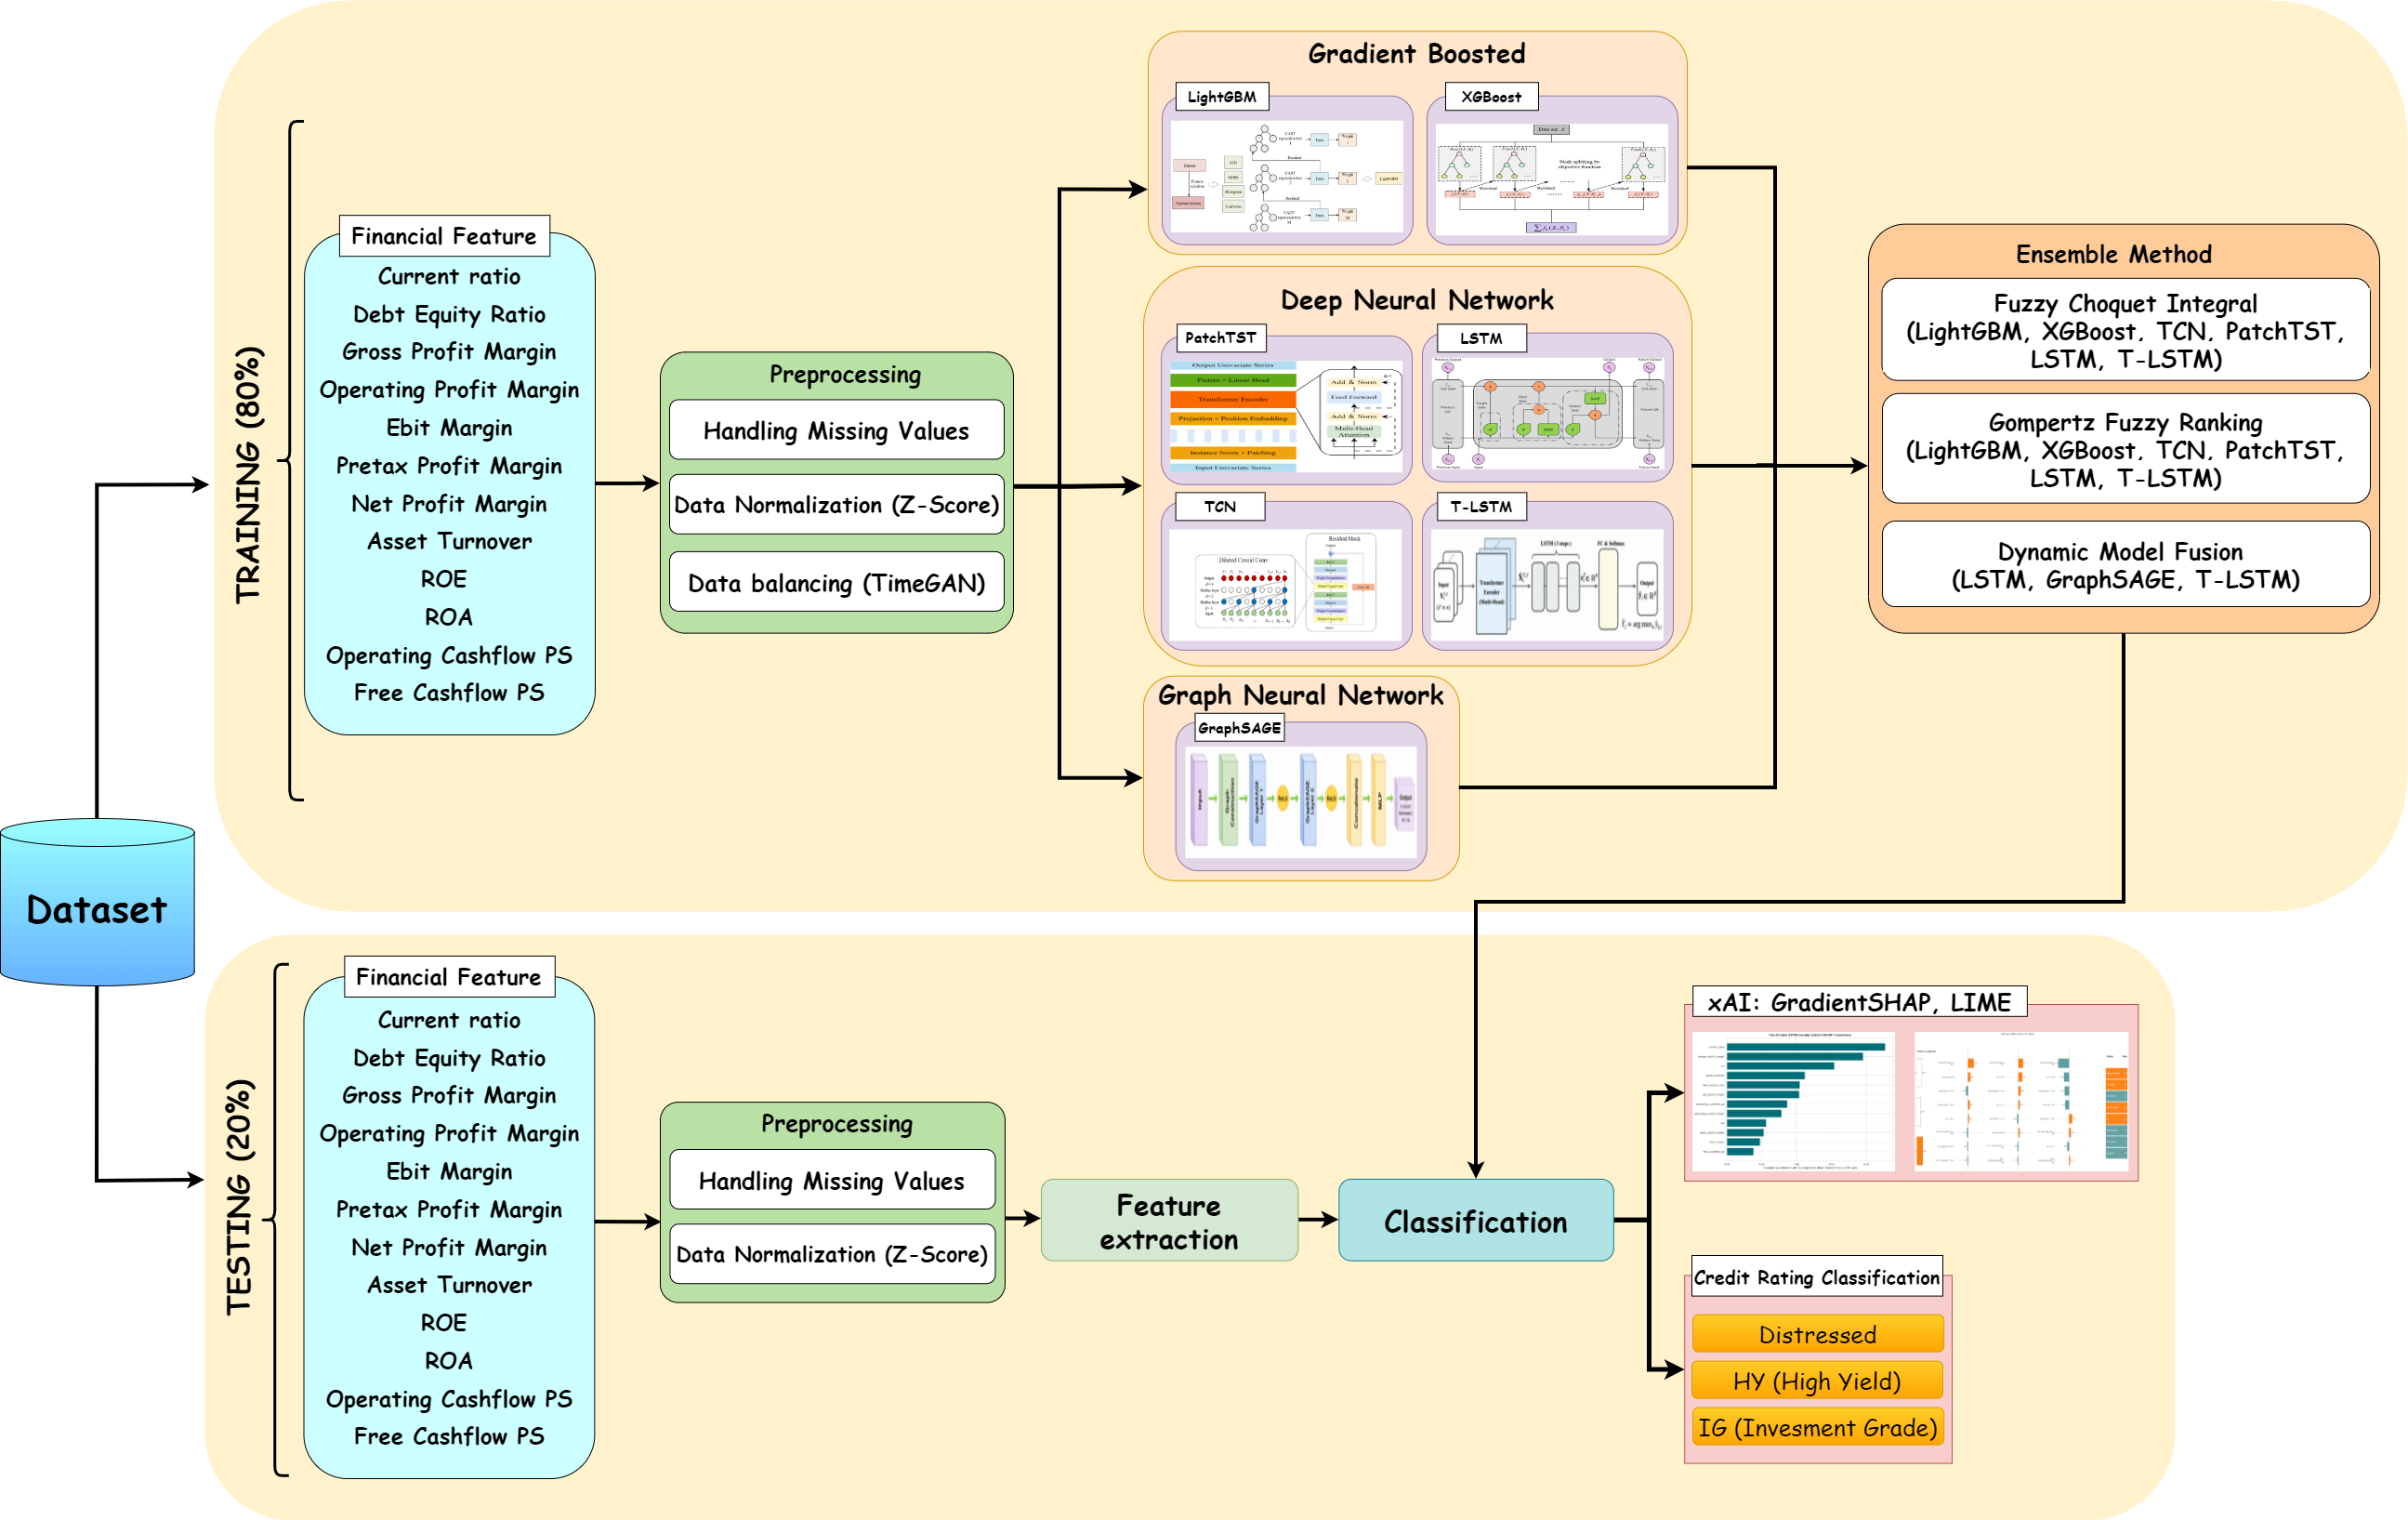
\includegraphics[width=\textwidth]{acc-loss/diagram_pipeline_overview.png}
    \caption{Mô hình đề xuất} % Dòng chú thích dưới ảnh
    \label{fig:proposed_model}
\end{figure}
\subsection{Pha huấn luyện} 
\subsubsection{Tiền xử lý dữ liệu và chuẩn bị dữ liệu} 
Tiền xử lý dữ liệu là bước quan trọng nhằm đảm bảo dữ liệu đầu vào phù hợp với bài toán xếp hạng tín dụng doanh nghiệp và giúp các mô hình học ổn định hơn. Trong nghiên cứu này, dữ liệu được xử lý từ bộ 12 chỉ số tài chính phản ánh thanh khoản, đòn bẩy, khả năng sinh lời, hiệu quả hoạt động và dòng tiền. Trước hết, các bản ghi trùng lặp theo mã chứng khoán và ngày xếp hạng được gộp lại, đồng thời các giá trị khuyết thiếu được điền bằng trung vị của tập huấn luyện nhằm hạn chế ảnh hưởng của ngoại lai và tránh rò rỉ dữ liệu.

Tiếp theo, các đặc trưng tài chính có phân phối lệch được biến đổi để giảm độ lệch, sau đó dữ liệu được chuẩn hóa bằng Z-score nhằm đưa các chỉ số có thang đo khác nhau về cùng một hệ quy chiếu. Bên cạnh đó, bộ dữ liệu ban đầu gồm 21 hạng tín dụng riêng biệt, bao gồm: D, C, CC, CCC-, CCC, CCC+, B-, B, B+, BB-, BB, BB+, BBB-, BBB, BBB+, A-, A, A+, AA-, AA, AA+ và AAA. Do số lượng mẫu giữa các hạng có sự chênh lệch lớn, đặc biệt các hạng rủi ro cao xuất hiện ít hơn, nghiên cứu thực hiện gộp 21 hạng này thành ba nhóm chính: Distressed, High Yield (HY) và Investment Grade (IG). Cụ thể, nhóm Distressed bao gồm các hạng từ C đến CCC+, đại diện cho các doanh nghiệp có rủi ro tín dụng rất cao hoặc đang gặp khó khăn tài chính nghiêm trọng. Nhóm High Yield (HY) gồm các hạng từ B- đến BB+, phản ánh các doanh nghiệp có mức rủi ro trung bình đến cao nhưng chưa rơi vào tình trạng kiệt quệ. Nhóm Investment Grade (IG) gồm các hạng từ BBB- đến AAA, đại diện cho các doanh nghiệp có khả năng thanh toán tốt và mức rủi ro tín dụng thấp. Việc gộp lớp này giúp giảm tình trạng mất cân bằng dữ liệu, đồng thời phù hợp với mục tiêu phân loại rủi ro tín dụng theo ba mức chính. Cuối cùng, dữ liệu được cấu trúc thành các chuỗi thời gian theo từng doanh nghiệp thông qua kỹ thuật cửa sổ trượt. Các chuỗi này được sử dụng cho các mô hình học sâu chuỗi thời gian như LSTM, TCN, PatchTST và T-LSTM. Để cải thiện tình trạng mất cân bằng dữ liệu, đặc biệt ở nhóm Distressed, nghiên cứu sử dụng TimeGAN nhằm sinh thêm các chuỗi tài chính giả lập có đặc điểm tương tự dữ liệu gốc. Nhờ đó, tập huấn luyện trở nên cân bằng hơn, giúp mô hình cải thiện khả năng tổng quát hóa và nâng cao hiệu quả nhận diện các doanh nghiệp có rủi ro tín dụng cao.
\subsubsection{Rút trích đặc trưng và huấn luyện}
Sau khi dữ liệu được tiền xử lý, các chuỗi chỉ số tài chính được đưa vào các mô hình để rút trích đặc trưng và huấn luyện. Dữ liệu đầu vào được tổ chức theo dạng cửa sổ trượt, giúp mô hình khai thác sự thay đổi của doanh nghiệp qua nhiều kỳ thời gian liên tiếp. Quá trình rút trích đặc trưng được thực hiện tự động bởi các mô hình học sâu như LSTM, TCN, PatchTST và T-LSTM. Các mô hình này học trực tiếp từ chuỗi dữ liệu tài chính đã chuẩn hóa, bao gồm giá trị chỉ số, xu hướng biến động và mối quan hệ giữa các đặc trưng theo thời gian. Trong quá trình huấn luyện, các mô hình được huấn luyện độc lập trên cùng một tập dữ liệu và cùng quy trình tiền xử lý nhằm đảm bảo tính công bằng khi so sánh. Thuật toán AdamW được sử dụng để tối ưu trọng số, kết hợp với hàm mất mát Cross Entropy cho bài toán phân loại ba lớp IG, HY và Distressed. Để tăng độ ổn định và hạn chế quá khớp, kỹ thuật Gradient Clipping được áp dụng trong quá trình lan truyền ngược. Đồng thời, các chỉ số Loss, Accuracy và F1-score được theo dõi trên tập huấn luyện và tập validation. Việc lựa chọn mô hình dựa trên F1-score giúp đánh giá cân bằng hơn giữa các lớp, đặc biệt trong bối cảnh dữ liệu xếp hạng tín dụng có sự mất cân bằng.

\subsection{Pha kiểm thử}
Sau khi hoàn tất quá trình huấn luyện, các mô hình được đưa vào pha kiểm thử nhằm đánh giá khả năng tổng quát hóa trên dữ liệu chưa từng thấy. Trong giai đoạn này, mô hình được chuyển sang chế độ đánh giá để đảm bảo quá trình suy luận ổn định và không cập nhật tham số. Đầu ra của các mô hình là nhãn dự đoán thuộc ba nhóm xếp hạng tín dụng gồm IG, HY và Distressed. Pha kiểm thử được thực hiện trên cả các mô hình đơn lẻ và các kịch bản kết hợp. Các mô hình đơn lẻ bao gồm LightGBM, XGBoost, LSTM, TCN, PatchTST, T-LSTM và GraphSAGE. Bên cạnh đó, nghiên cứu xây dựng các tổ hợp Fuzzy Ensemble như TTX, PLL và TTLPXL, sử dụng Fuzzy Choquet Integral và Gompertz Fuzzy Ranking để kết hợp xác suất dự đoán của nhiều mô hình. Ngoài ra, các kịch bản Dynamic Model Fusion gồm DMF-LG, DMF-LT, DMF-TG và DMF-LTG được triển khai nhằm lựa chọn mô hình phù hợp theo từng mẫu dữ liệu thông qua cơ chế Dynamic Classifier Selection. Hiệu năng của các mô hình được đánh giá bằng nhiều chỉ số gồm Accuracy, Precision, Recall, F1-score, AUC-ROC, ma trận nhầm lẫn và thời gian kiểm thử. Các chỉ số này giúp đánh giá toàn diện khả năng phân loại tổng thể cũng như hiệu quả nhận diện từng lớp xếp hạng tín dụng. Đặc biệt, ma trận nhầm lẫn được sử dụng để phân tích chi tiết các lỗi dự đoán giữa ba nhóm IG, HY và Distressed. Bên cạnh đánh giá hiệu suất, pha kiểm thử còn tích hợp các phương pháp Explainable AI gồm GradientSHAP và LIME. GradientSHAP được sử dụng để xác định mức độ ảnh hưởng của từng chỉ số tài chính đến kết quả dự đoán, trong khi LIME hỗ trợ giải thích cục bộ cho từng trường hợp doanh nghiệp cụ thể. Nhờ đó, kết quả kiểm thử không chỉ thể hiện hiệu quả phân loại của mô hình mà còn cung cấp cơ sở diễn giải, giúp tăng tính minh bạch và độ tin cậy của hệ thống xếp hạng tín dụng doanh nghiệp.


\section{KẾT QUẢ THỰC NGHIỆM}

\subsection{Môi trường cài đặt và tập dữ liệu thực nghiệm}

\subsubsection{Môi trường cài đặt}
Các thử nghiệm được thực hiện trên Kaggle Notebooks \cite{noauthor_notebooks_nodate}, sử dụng CPU Intel Xeon 2,00 GHz với 4 vCPU, 32 GB RAM và GPU NVIDIA Tesla P100 với 16 GB VRAM. Các mô hình được triển khai bằng Python 3.8+ và PyTorch. Pandas và NumPy được sử dụng để xử lý dữ liệu; Matplotlib và Scikit-learn hỗ trợ trực quan hóa và đánh giá. Giới hạn thời gian GPU của Kaggle được xem xét khi lựa chọn kích thước lô và cấu hình bộ nhớ.

\subsubsection{Tập dữ liệu thực nghiệm}
Tập dữ liệu được tổng hợp từ hai nguồn công khai trên Kaggle: \textit{Corporate Credit Rating} \cite{noauthor_corporate_credit_rating_nodate} và \textit{Corporate Credit Rating with Financial Ratios} \cite{noauthor_corporate_financial_ratios_nodate}. Hai nguồn được liên kết theo tên công ty, mã chứng khoán, tổ chức xếp hạng và ngày xếp hạng. Sau khi làm sạch, hợp nhất và loại bỏ bản ghi trùng lặp, dữ liệu gồm 8.680 quan sát của 1.623 doanh nghiệp trong giai đoạn 2005--2016. Mỗi quan sát gồm 12 chỉ số tài chính: Current Ratio, Debt-to-Equity Ratio, Gross Profit Margin, Operating Profit Margin, EBIT Margin, Pretax Profit Margin, Net Profit Margin, ROE, ROA, Asset Turnover, Operating Cash Flow per Share và Free Cash Flow per Share. Các chỉ số đại diện cho thanh khoản, đòn bẩy, khả năng sinh lời, hiệu quả hoạt động và dòng tiền. Hai mươi mốt hạng tín dụng ban đầu được gộp thành ba nhóm IG, HY và Distressed. Mỗi doanh nghiệp có trung bình khoảng 5,35 lần xếp hạng, vì vậy dữ liệu có cả cấu trúc bảng và yếu tố thời gian. Để hạn chế rò rỉ dữ liệu giữa các doanh nghiệp, tập huấn luyện, tập xác thực và tập kiểm thử được chia độc lập theo mã chứng khoán. Phân bố lớp sau khi gộp nhãn được trình bày trong Bảng~\ref{tab:class_distribution}.
\begin{table}[H] 
\centering 
\caption{Thông tin chi tiết về số dữ liệu của từng lớp ban đầu} 
\label{tab:class_distribution} 
\begin{tabular}{lccc} 
\hline \textbf{Lớp} & \textbf{Train} & \textbf{Val} & \textbf{Test} \\ \hline Investment Grade (IG) & 3898 & 557 & 1114 \\ High Yield (HY) & 1970 & 281 & 563 \\ Distressed & 208 & 30 & 59 \\ \hline 
\end{tabular} 
\end{table}
\subsection{Kịch bản thực nghiệm}

Mười bốn kịch bản thực nghiệm được chia thành hai nhóm. Nhóm thứ nhất gồm bảy mô hình đơn, mô hình lai và mô hình đồ thị: LightGBM, XGBoost, TCN, LSTM, PatchTST, T-LSTM và GraphSAGE. Nhóm thứ hai gồm bảy kịch bản học tập hợp sử dụng Tích phân Choquet mờ (FI), Xếp hạng mờ Gompertz (FR) hoặc Dynamic Model Fusion (DMF). Cấu hình từng kịch bản được trình bày trong Bảng~\ref{tab:experimental_scenarios}.

\begingroup
\centering
\begin{longtable}{c l l >{\raggedright\arraybackslash}p{6.5cm}}
\caption{Các kịch bản thực nghiệm}
\label{tab:experimental_scenarios}\\
\hline 
\textbf{Kịch bản} & \textbf{Tên kịch bản} & \textbf{Phương pháp kết hợp} & \textbf{Mô hình sử dụng} \\ \hline 
1 & LightGBM & -- & LightGBM \\ 
2 & XGBoost & -- & XGBoost \\ 
3 & TCN & -- & Temporal Convolutional Networks (TCN) \\ 
4 & LSTM & -- & Long Short-Term Memory (LSTM) \\ 
5 & PatchTST & -- & Patch Time Series Transformer (PatchTST) \\ 
6 & T-LSTM & -- & Transformer--Long Short-Term Memory (T-LSTM) \\ 
7 & GraphSAGE & -- & GraphSAGE, Multilayer Perceptron (MLP) \\ 
8 & FI-TTX & Fuzzy Choquet Integral & TCN + T-LSTM + XGBoost \\ 
9 & FI-PLL & Fuzzy Choquet Integral & PatchTST + LSTM + LightGBM \\ 
10 & FI-TTLPXL & Fuzzy Choquet Integral & TCN + T-LSTM + LSTM + PatchTST + XGBoost + LightGBM \\ 
11 & FR-TTX & Gompertz Fuzzy Ranking & TCN + T-LSTM + XGBoost \\ 
12 & FR-PLL & Gompertz Fuzzy Ranking & PatchTST + LSTM + LightGBM \\ 
13 & FR-TTLPXL & Gompertz Fuzzy Ranking & TCN + T-LSTM + LSTM + PatchTST + XGBoost + LightGBM \\ 
14 & DMF-LG & Dynamic Model Fusion & LSTM + GraphSAGE \\ 
15 & DMF-LT & Dynamic Model Fusion & LSTM + T-LSTM \\ 
16 & DMF-TG & Dynamic Model Fusion & T-LSTM + GraphSAGE \\
17 & DMF-LTG & Dynamic Model Fusion & LSTM + T-LSTM +GraphSAGE \\ \hline
\end{longtable}
\endgroup

\begin{table}[H] 
\centering 
\caption{Tham số huấn luyện các kịch bản} 
\label{tab:hyperparameter} 
\begin{tabular}{c c c l c} 
\hline 
\textbf{Kịch bản} & \textbf{Tốc độ học} & \textbf{Số epoch} & \textbf{Hàm mất mát} & \textbf{Số lớp} \\ 
\hline 
1 & 3e-2 & 100 & Cross Entropy & 3 \\ 
2 & 3e-2 & 100 & Cross Entropy & 3 \\ 
3 & 3e-4 & 100 & Cross Entropy & 3 \\ 
4 & 3e-4 & 100 & Cross Entropy & 3 \\ 
5 & 3e-4 & 100 & Cross Entropy & 3 \\ 
6 & 3e-4 & 100 & Cross Entropy & 3 \\ 
7 & 6e-4 & 100 & Cross Entropy & 3 \\ 
\hline 
\end{tabular} 
\end{table}

Bảng~\ref{tab:hyperparameter} trình bày các tham số huấn luyện được thiết lập cho từng kịch bản thực nghiệm. Đối với LightGBM và XGBoost, tốc độ học $3\times10^{-2}$ được sử dụng trong cơ chế boosting nhằm điều chỉnh mức đóng góp của từng cây quyết định vào mô hình tổng thể; số lần học tương ứng với số vòng boosting. Với các mô hình học sâu như TCN, LSTM, PatchTST và T-LSTM, tốc độ học nhỏ hơn, $3\times10^{-4}$, được lựa chọn để giúp quá trình cập nhật trọng số ổn định và hạn chế dao động khi xử lý dữ liệu chuỗi thời gian tài chính. Riêng GraphSAGE sử dụng thuật toán AdamW với tốc độ học $6\times10^{-4}$ nhằm ổn định quá trình học biểu diễn nút trên đồ thị. Tất cả các kịch bản đều sử dụng hàm mất mát Cross Entropy cho bài toán phân loại đa lớp gồm ba nhóm xếp hạng tín dụng: Distressed, HY và IG.
\subsection{Kết quả huấn luyện}

\begin{table}[H]
\centering
\caption{Bảng tổng hợp kết quả huấn luyện của các mô hình (\%)}
\label{tab:training_results}
\begin{tabular}{c l c c c c}
\hline
\textbf{Kịch bản} & \textbf{Mạng huấn luyện} & \textbf{Train Loss} & \textbf{Val Loss} & \textbf{Train Acc} & \textbf{Val Acc} \\
\hline
1 & LightGBM  & 0.123 & 0.266 & 94.0 & 92.0 \\
2 & XGBoost   & 0.177 & 0.267 & 94.0 & 92.4 \\
3 & TCN       & 0.248 & 0.276 & 92.7 & 92.3 \\
4 & LSTM      & 0.190 & 0.268 & 94.0 & 92.2 \\
5 & PatchTST  & 0.217 & 0.279 & 93.2 & 91.7 \\
6 & T-LSTM    & 0.167 & 0.223 & 94.0 & 92.4 \\
7 & GraphSAGE & 0.343 & 0.399 & 92.1 & 92.2 \\
\hline
\end{tabular}
\end{table}
\subsubsection{Độ chính xác (Accuracy)}
\begin{figure}[H]
    \centering % Căn giữa hình ảnh
    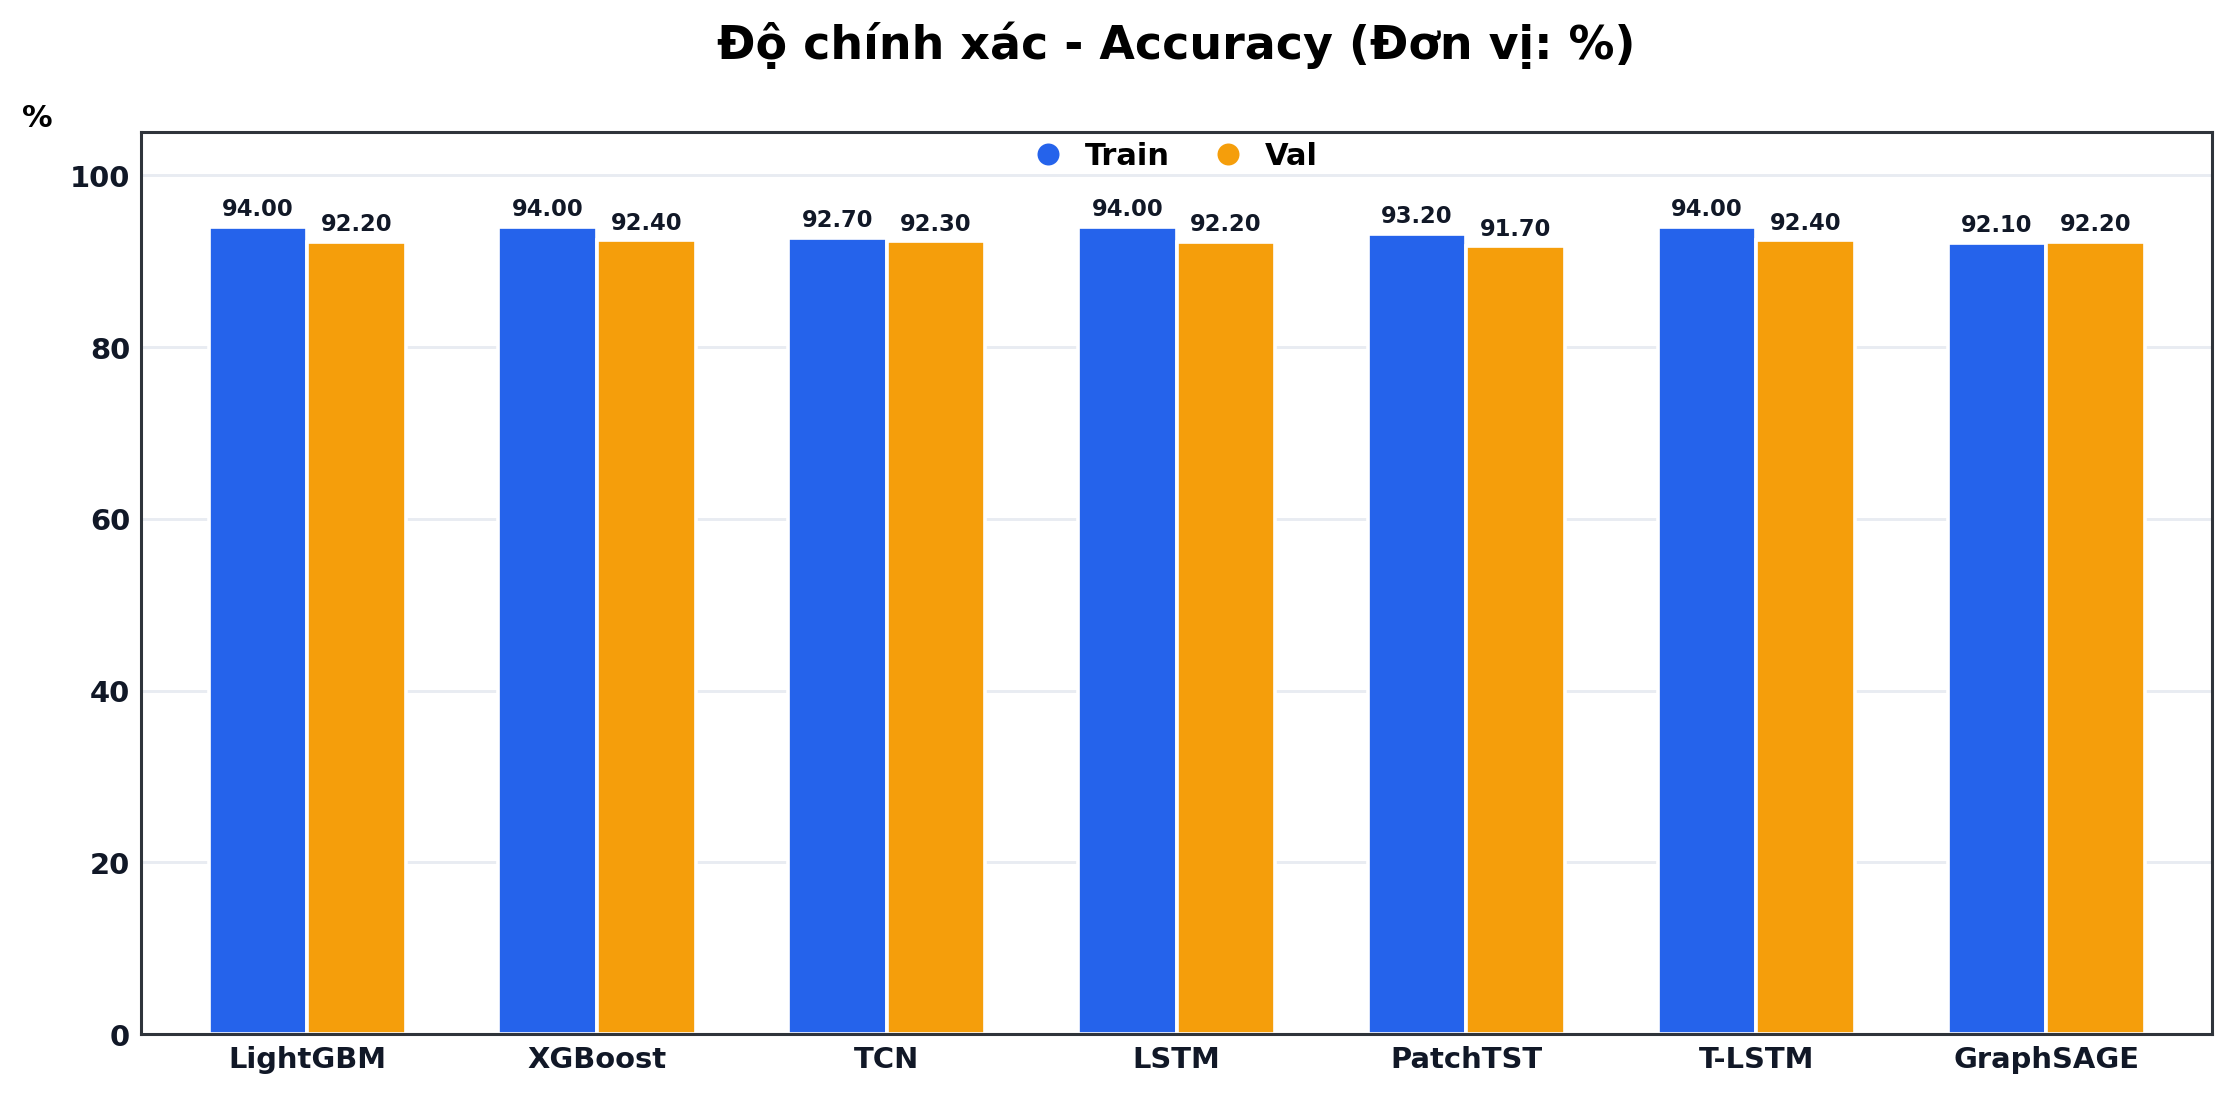
\includegraphics[width=\fairfigurewidth]{acc-loss/curve_accuracy_overall.png}
    \caption{Biểu đồ độ chính xác} % Dòng chú thích dưới ảnh
    \label{tab:acc-train}
\end{figure}

Hình~\ref{tab:acc-train} cho thấy Accuracy trên tập huấn luyện nằm trong khoảng 92,10\%--94,00\%, còn trên tập xác thực nằm trong khoảng 91,70\%--92,40\%. XGBoost và T-LSTM cùng đạt Accuracy xác thực cao nhất, ở mức 92,40\%. TCN và GraphSAGE có chênh lệch giữa hai tập lần lượt là 0,40 và 0,10 điểm phần trăm. PatchTST đạt Accuracy xác thực thấp nhất với 91,70\%. Khoảng biến thiên 0,70 điểm phần trăm cho thấy khác biệt giữa các mô hình trên tập xác thực tương đối nhỏ. Biểu đồ độ chính xác trong quá trình huấn luyện được trình bày chi tiết ở Bảng~\ref{tab:accuracy_models}.

\begingroup
\centering
\renewcommand{\arraystretch}{1.2}
\setlength{\tabcolsep}{0pt}
\begin{longtable}{>{\centering\arraybackslash}p{0.48\textwidth}|
                  >{\centering\arraybackslash}p{0.48\textwidth}}
\caption{Độ chính xác của các mô hình}
\label{tab:accuracy_models}\\
\hline
\modelcurvecell{Kịch bản 1: LightGBM}{acc-loss/curve_accuracy_lightgbm.png} &
\modelcurvecell{Kịch bản 2: XGBoost}{acc-loss/curve_accuracy_xgboost.png} \\
\hline
\modelcurvecell{Kịch bản 3: TCN}{acc-loss/curve_accuracy_tcn.png} &
\modelcurvecell{Kịch bản 4: LSTM}{acc-loss/curve_accuracy_lstm.png} \\
\hline
\modelcurvecell{Kịch bản 5: PatchTST}{acc-loss/curve_accuracy_patchtst.png} &
\modelcurvecell{Kịch bản 6: T-LSTM}{acc-loss/curve_accuracy_tlstm.png} \\
\hline
\modelcurvecell{Kịch bản 7: GraphSAGE}{acc-loss/curve_accuracy_graphsage.png} & \\
\hline
\end{longtable}
\endgroup


\subsubsection{Độ mất mát (loss)}
\begin{figure}[H]
    \centering % Căn giữa hình ảnh
    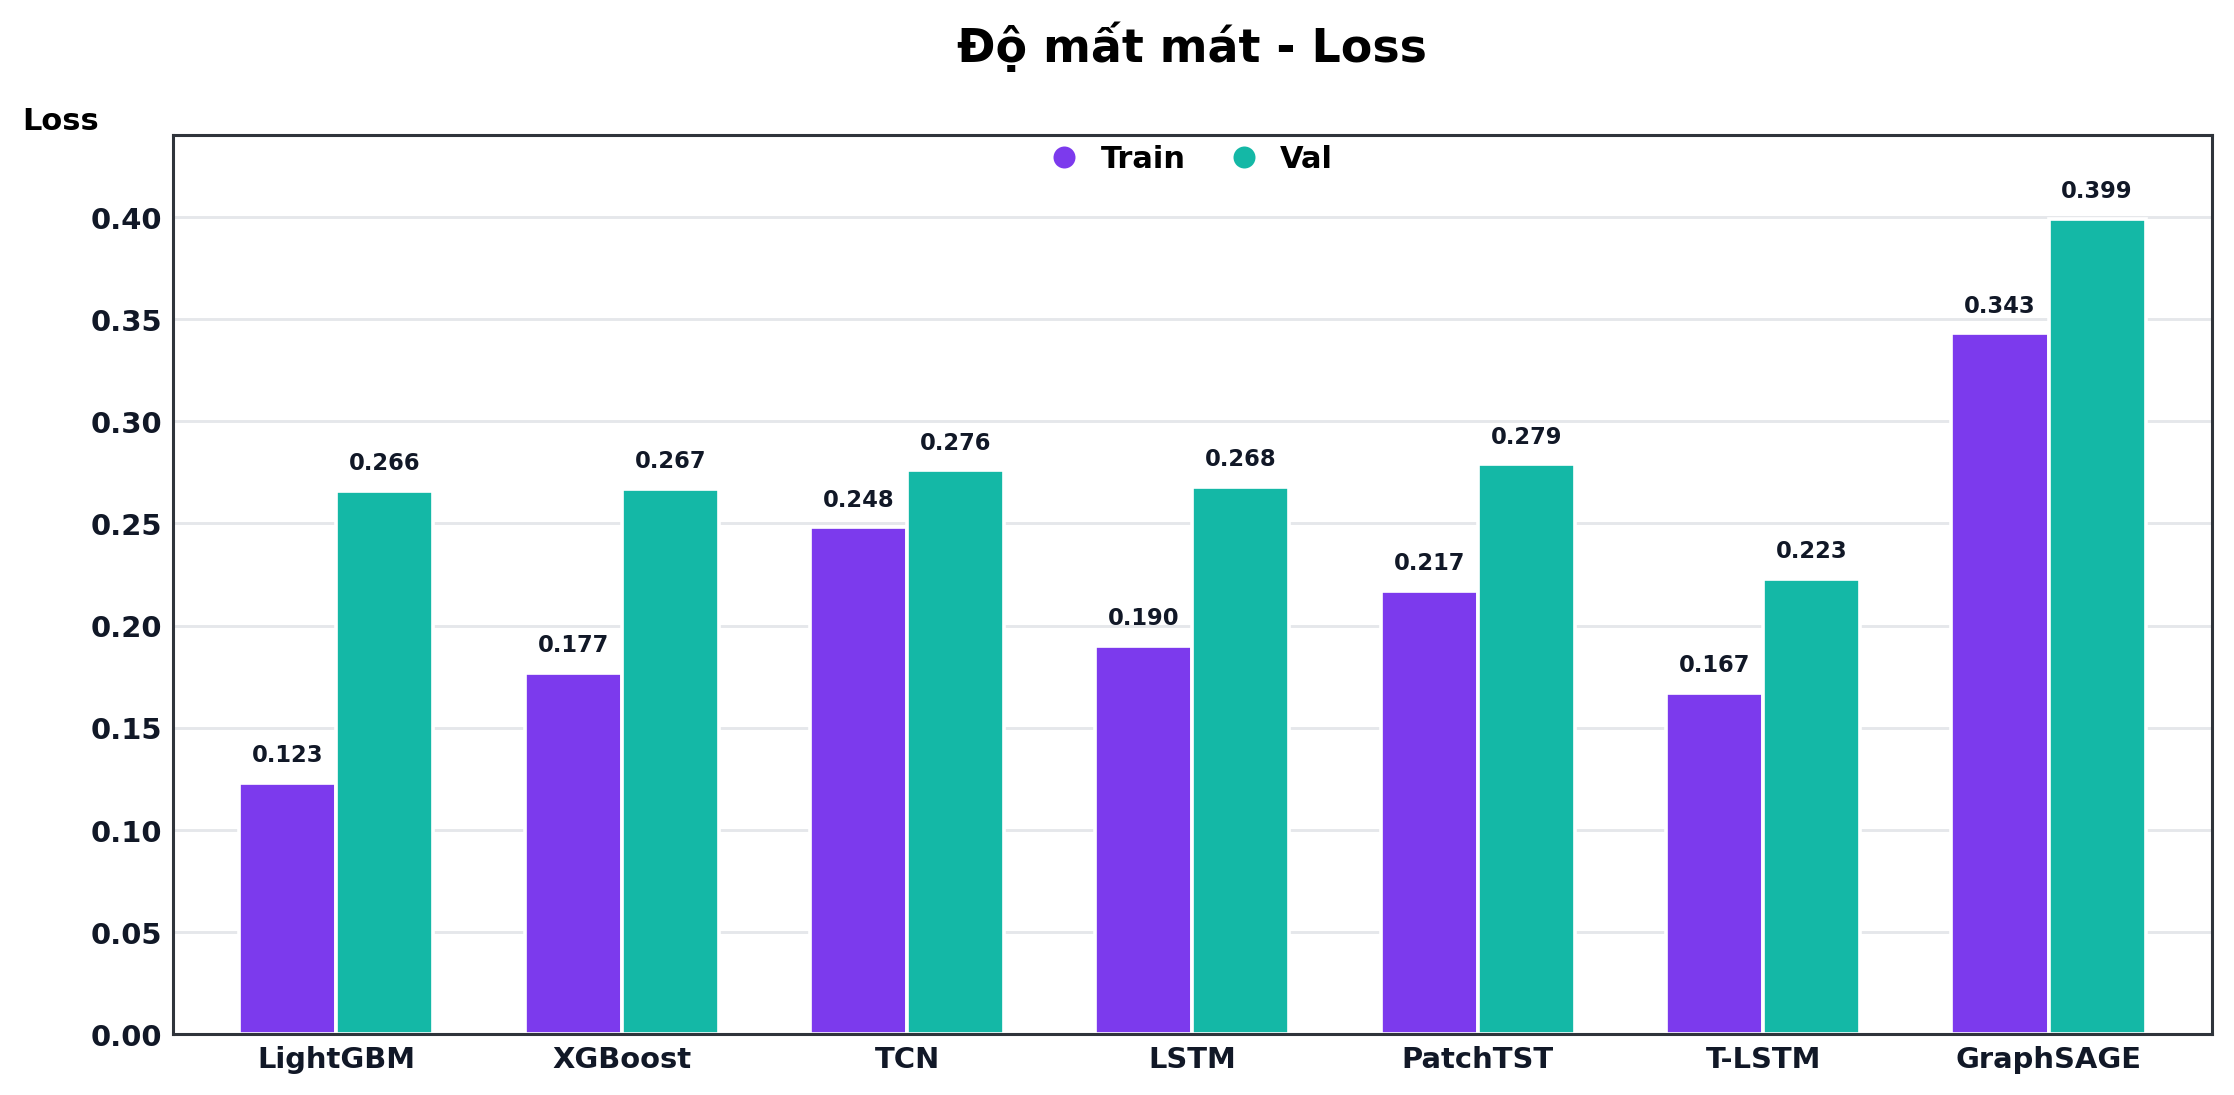
\includegraphics[width=\fairfigurewidth]{acc-loss/curve_loss_overall.png}
    \caption{Biểu đồ độ mất mát} % Dòng chú thích dưới ảnh
\end{figure}

Độ mất mát trên tập huấn luyện dao động từ 0,123 đến 0,343; trên tập xác thực, giá trị này dao động từ 0,223 đến 0,399. T-LSTM có hàm mất mát xác thực thấp nhất (0,223), tiếp theo là LightGBM (0,266), XGBoost (0,267) và LSTM (0,268). GraphSAGE ghi nhận giá trị cao nhất trên cả tập huấn luyện (0,343) và tập xác thực (0,399). Các kết quả mô tả này cho thấy T-LSTM duy trì giá trị hàm mất mát thấp trên tập xác thực, nhưng chưa đủ để kết luận khác biệt có ý nghĩa thống kê giữa các mô hình. Biểu đồ độ mất mát trong quá trình huấn luyện được trình bày chi tiết ở Bảng~\ref{tab:loss_models}.

\begingroup
\centering
\renewcommand{\arraystretch}{1.2}
\setlength{\tabcolsep}{0pt}
\begin{longtable}{>{\centering\arraybackslash}p{0.48\textwidth}|
                  >{\centering\arraybackslash}p{0.48\textwidth}}
\caption{Độ mất mát của các mô hình}
\label{tab:loss_models}\\
\hline

\modelcurvecell{Kịch bản 1: LightGBM}{acc-loss/curve_loss_lightgbm.png} &
\modelcurvecell{Kịch bản 2: XGBoost}{acc-loss/curve_loss_xgboost.png} \\
\hline

\modelcurvecell{Kịch bản 3: TCN}{acc-loss/curve_loss_tcn.png} &
\modelcurvecell{Kịch bản 4: LSTM}{acc-loss/curve_loss_lstm.png} \\
\hline

\modelcurvecell{Kịch bản 5: PatchTST}{acc-loss/curve_loss_patchtst.png} &
\modelcurvecell{Kịch bản 6: T-LSTM}{acc-loss/curve_loss_tlstm.png} \\
\hline

\modelcurvecell{Kịch bản 7: GraphSAGE}{acc-loss/curve_loss_graphsage.png} & \\
\hline
\end{longtable}
\endgroup

\subsubsection{Thời gian huấn luyện}

\begin{figure}[H]
    \centering % Căn giữa hình ảnh
    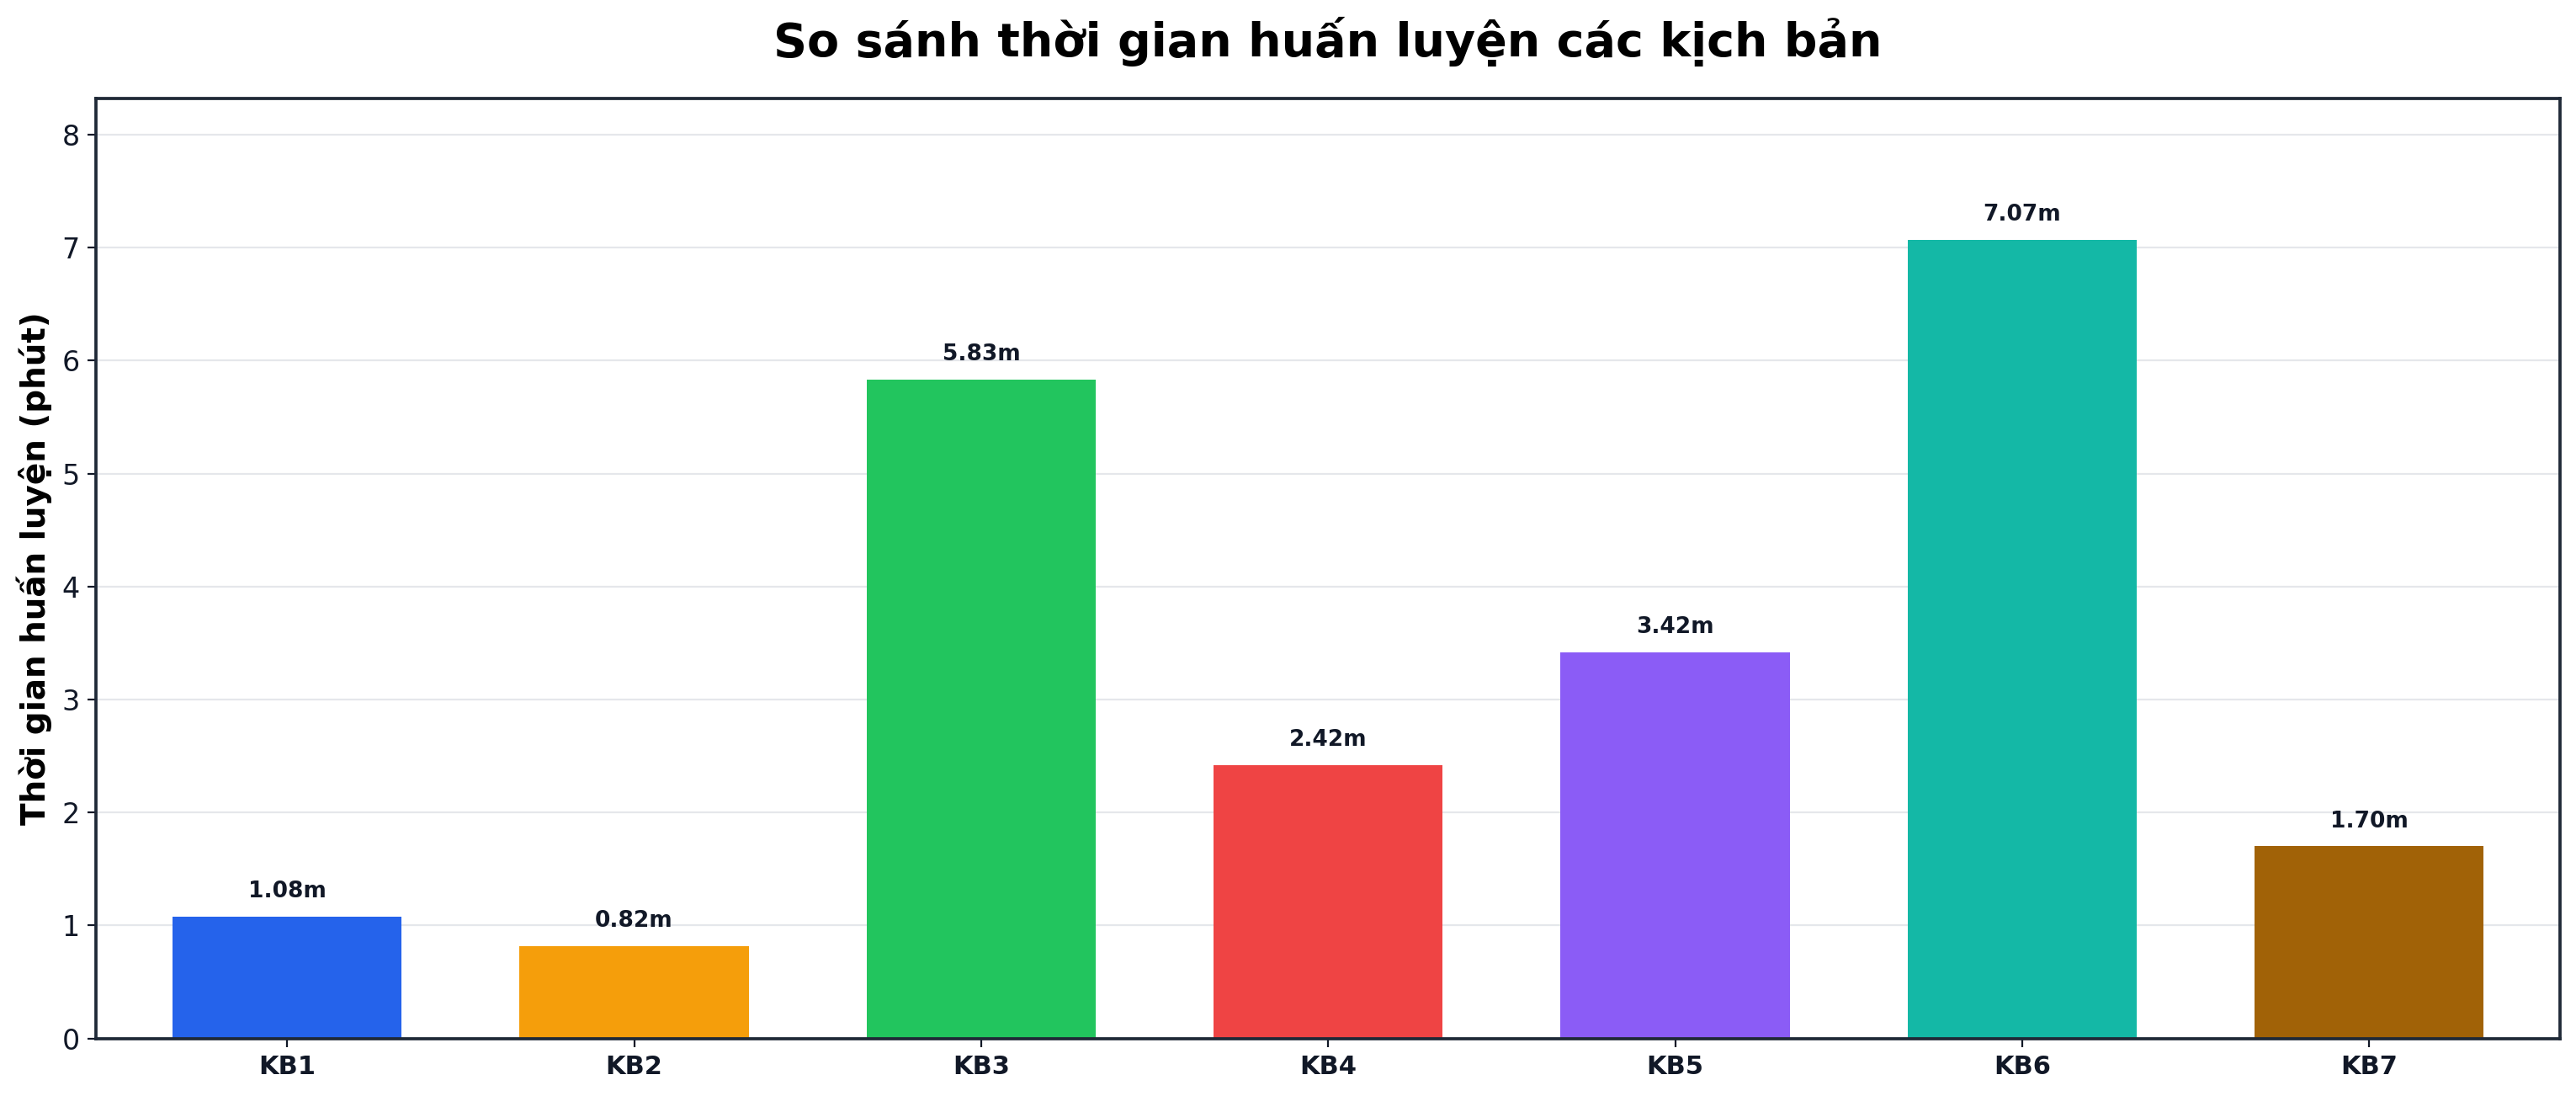
\includegraphics[width=\fairfigurewidth]{acc-loss/metric_training_time.png}
    \caption{Thời gian huấn luyện các kịch bản } 
\end{figure}

Thời gian huấn luyện khác nhau đáng kể giữa các kiến trúc. T-LSTM và TCN có thời gian cao nhất, lần lượt là 7,07 và 5,83 phút. PatchTST, LSTM và GraphSAGE lần lượt cần 3,42, 2,42 và 1,70 phút; XGBoost và LightGBM cần 0,82 và 1,08 phút. Kết quả phản ánh sự đánh đổi giữa chi phí huấn luyện của các mô hình chuỗi và tốc độ của các mô hình cây tăng cường trong môi trường thực nghiệm đã sử dụng.

\subsection{Kết quả kiểm thử}

\subsubsection{Độ chính xác}
\begin{figure}[H]
    \centering % Căn giữa hình ảnh
    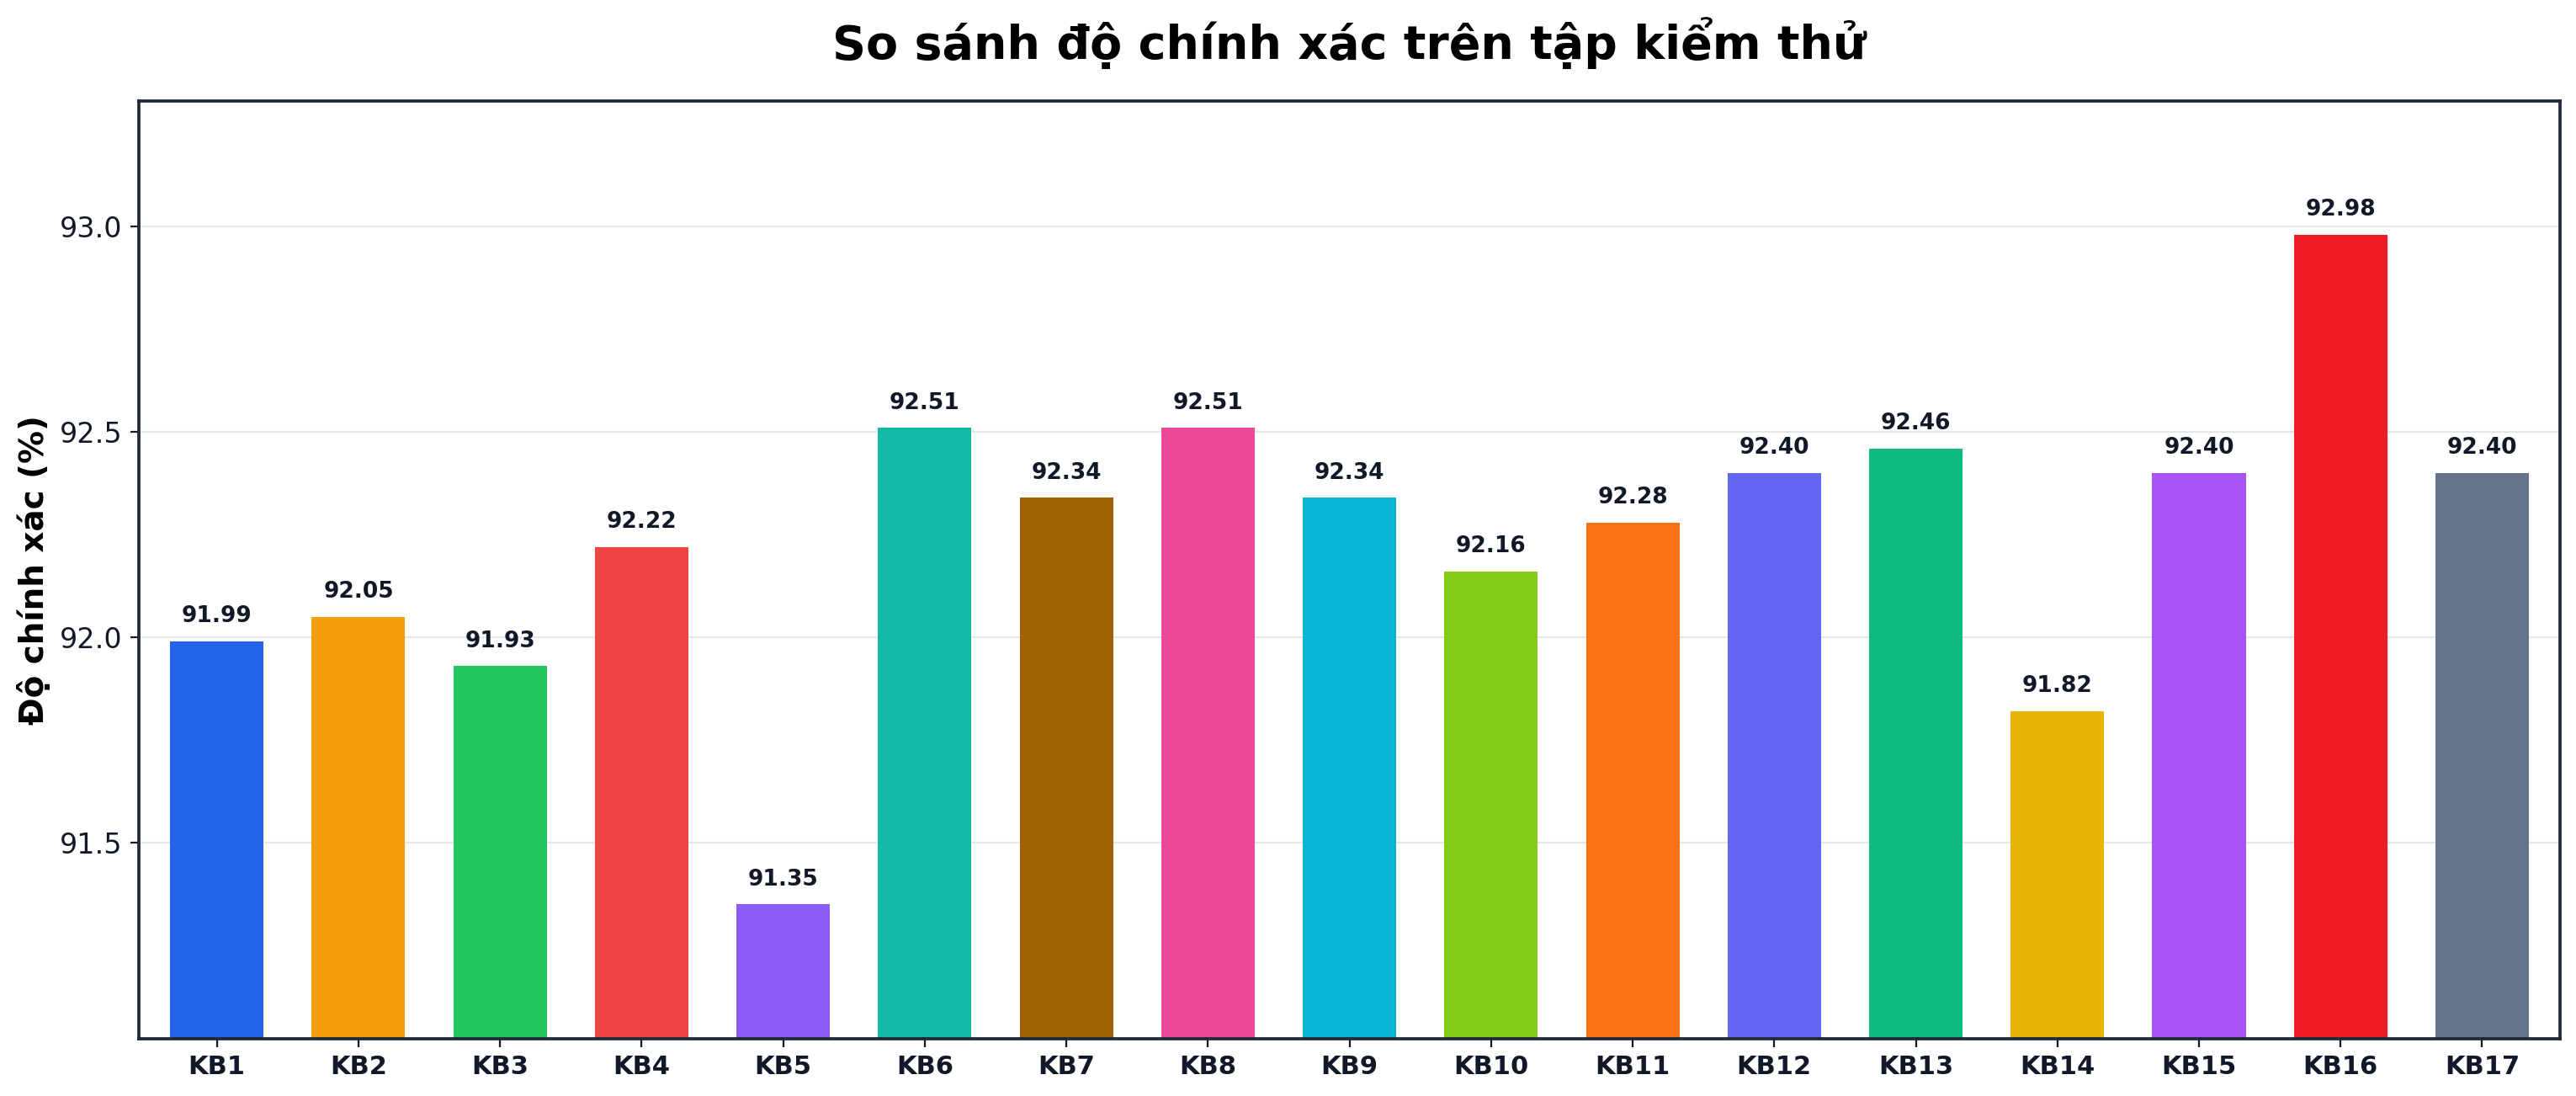
\includegraphics[width=\fairfigurewidth]{acc-loss/metric_accuracy_test_scenarios.png}
    \caption{Biểu đồ độ chính xác trên tập kiểm thử} 
    \label{tab:acc-test}
\end{figure}
Kết quả thực nghiệm cho thấy độ chính xác của 17 mô hình và kịch bản kết hợp trên tập kiểm thử dao động từ 91,35\% đến 92,98\%. Nhìn chung, tất cả các mô hình đều đạt trên 91\%, cho thấy khả năng phân loại xếp hạng tín dụng doanh nghiệp tương đối ổn định. Trong nhóm mô hình đơn lẻ, T-LSTM đạt kết quả cao nhất với 92,51\%, tiếp theo là GraphSAGE với 92,34\% và LSTM với 92,22\%. Các mô hình học máy dạng bảng như LightGBM và XGBoost cũng cho kết quả tốt, lần lượt đạt 91,99\% và 92,05\%. Đối với nhóm Fuzzy Ensemble, FI-TTX đạt độ chính xác cao nhất với 92,51\%, trong khi FR-TTLPXL đạt 92,46\%, cho thấy các phương pháp kết hợp mờ giúp duy trì hiệu suất ổn định. Trong nhóm Dynamic Model Fusion, DMF-TG đạt kết quả tốt nhất toàn bộ biểu đồ với 92,98\%. Kết quả này cho thấy cơ chế kết hợp động giữa các mô hình có khả năng khai thác hiệu quả thông tin bổ sung, đặc biệt khi kết hợp mô hình chuỗi thời gian và mô hình đồ thị.

\subsubsection{Ma trận nhầm lẫn}

\begingroup
\renewcommand{\arraystretch}{1.2}
\setlength{\tabcolsep}{4pt}
\begin{longtable}{>{\centering\arraybackslash}m{0.31\textwidth}
                   >{\centering\arraybackslash}m{0.31\textwidth}
                   >{\centering\arraybackslash}m{0.31\textwidth}}
\caption{Ma trận nhầm lẫn các kịch bản trên tập kiểm thử}
\label{tab:confusion_matrices}\\

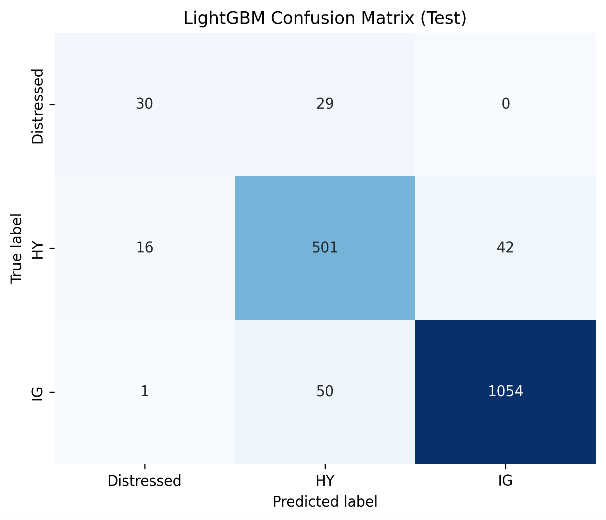
\includegraphics[width=0.95\linewidth]{acc-loss/confusion_lightgbm.png} &
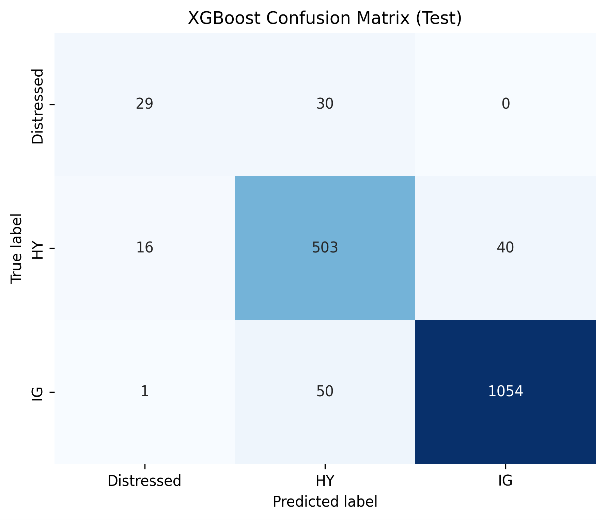
\includegraphics[width=0.95\linewidth]{acc-loss/confusion_xgboost.png} &
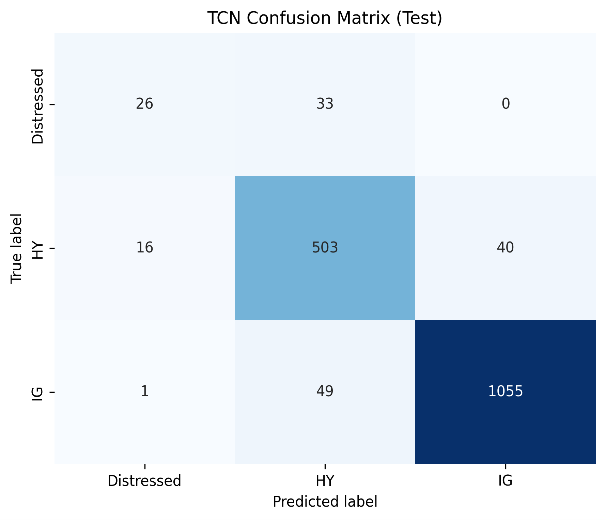
\includegraphics[width=0.95\linewidth]{acc-loss/confusion_tcn.png} \\


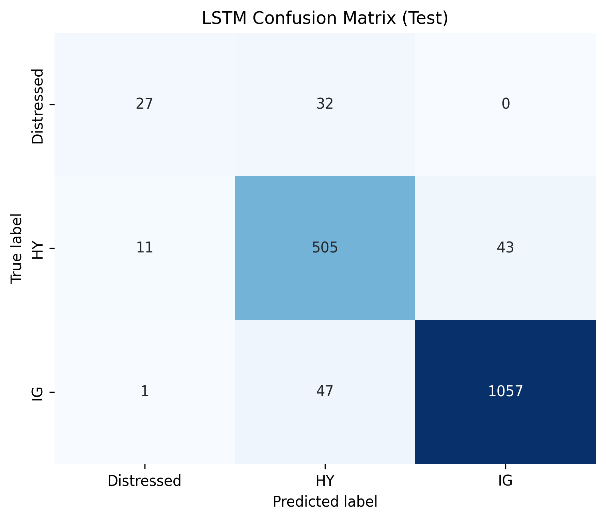
\includegraphics[width=0.95\linewidth]{acc-loss/confusion_lstm.png} &
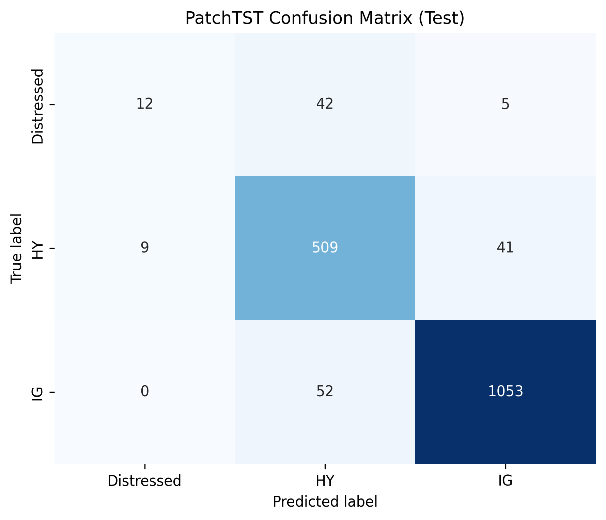
\includegraphics[width=0.95\linewidth]{acc-loss/confusion_patchtst.png} &
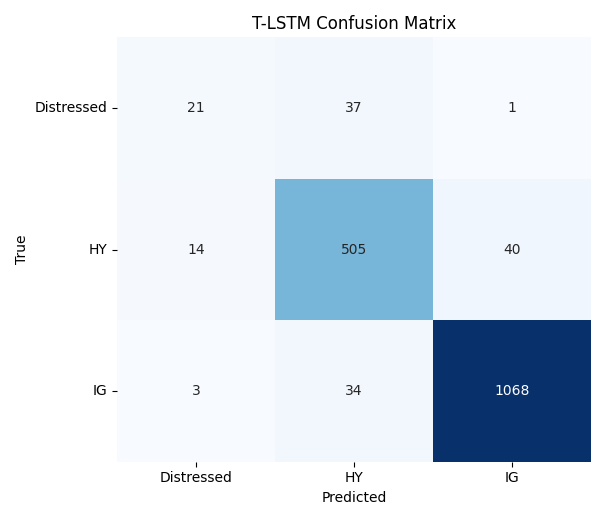
\includegraphics[width=0.95\linewidth]{acc-loss/confusion_tlstm.png} \\


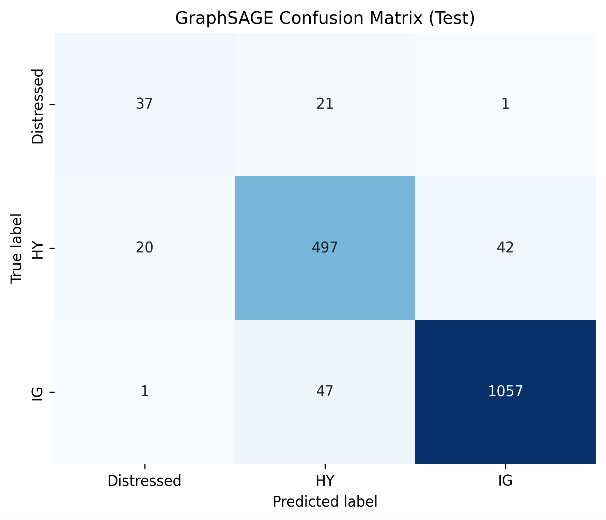
\includegraphics[width=0.95\linewidth]{acc-loss/confusion_graphsage.png} & 
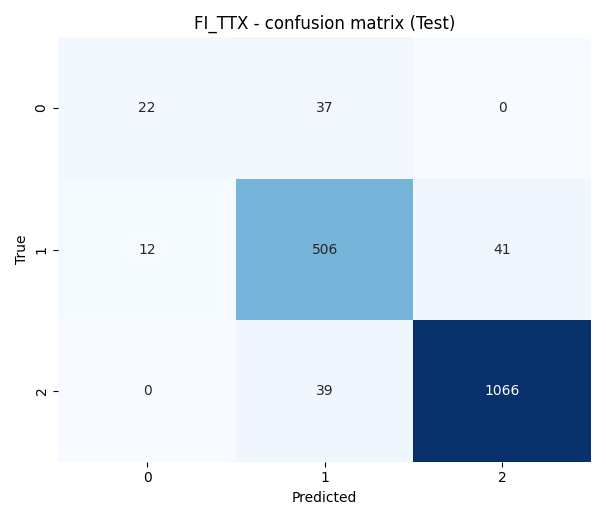
\includegraphics[width=0.95\linewidth]{acc-loss/confusion_fi_ttx.png} &
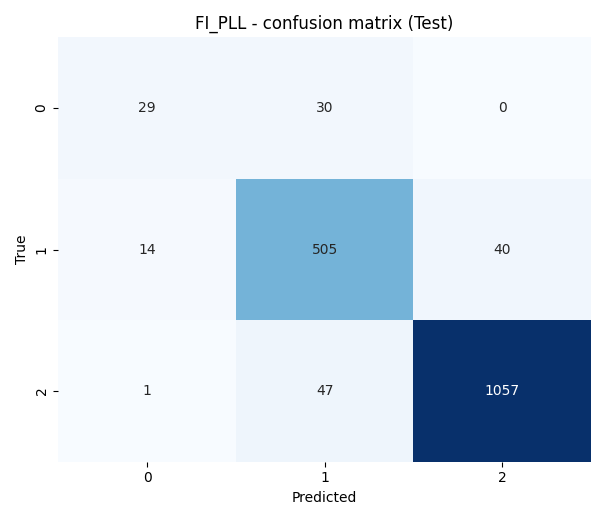
\includegraphics[width=0.95\linewidth]{acc-loss/confusion_fi_pll.png} \\


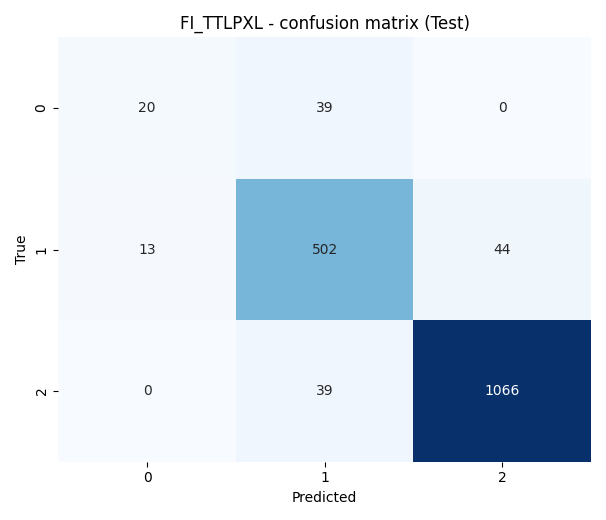
\includegraphics[width=0.95\linewidth]{acc-loss/confusion_fi_ttlpxl.png} & 
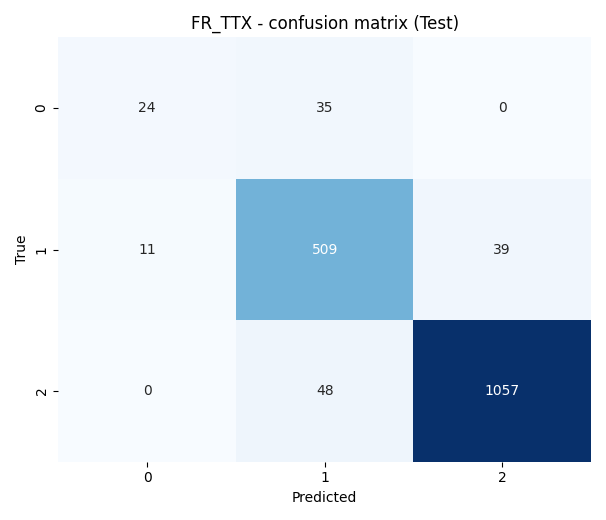
\includegraphics[width=0.95\linewidth]{acc-loss/confusion_fr_ttx.png} &
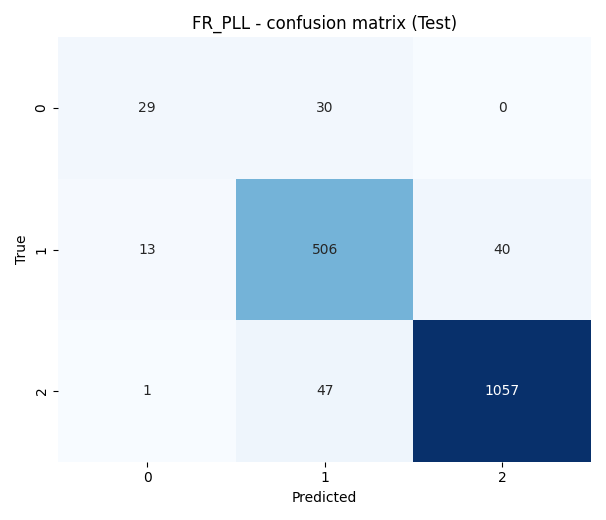
\includegraphics[width=0.95\linewidth]{acc-loss/confusion_fr_pll.png} \\


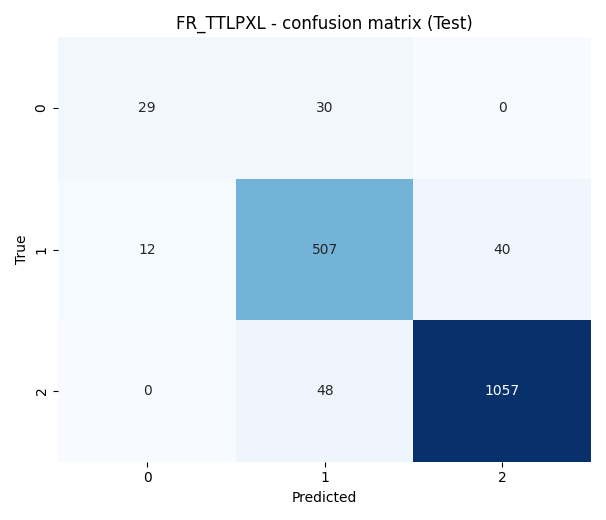
\includegraphics[width=0.95\linewidth]{acc-loss/confusion_fr_ttlpxl.png} &
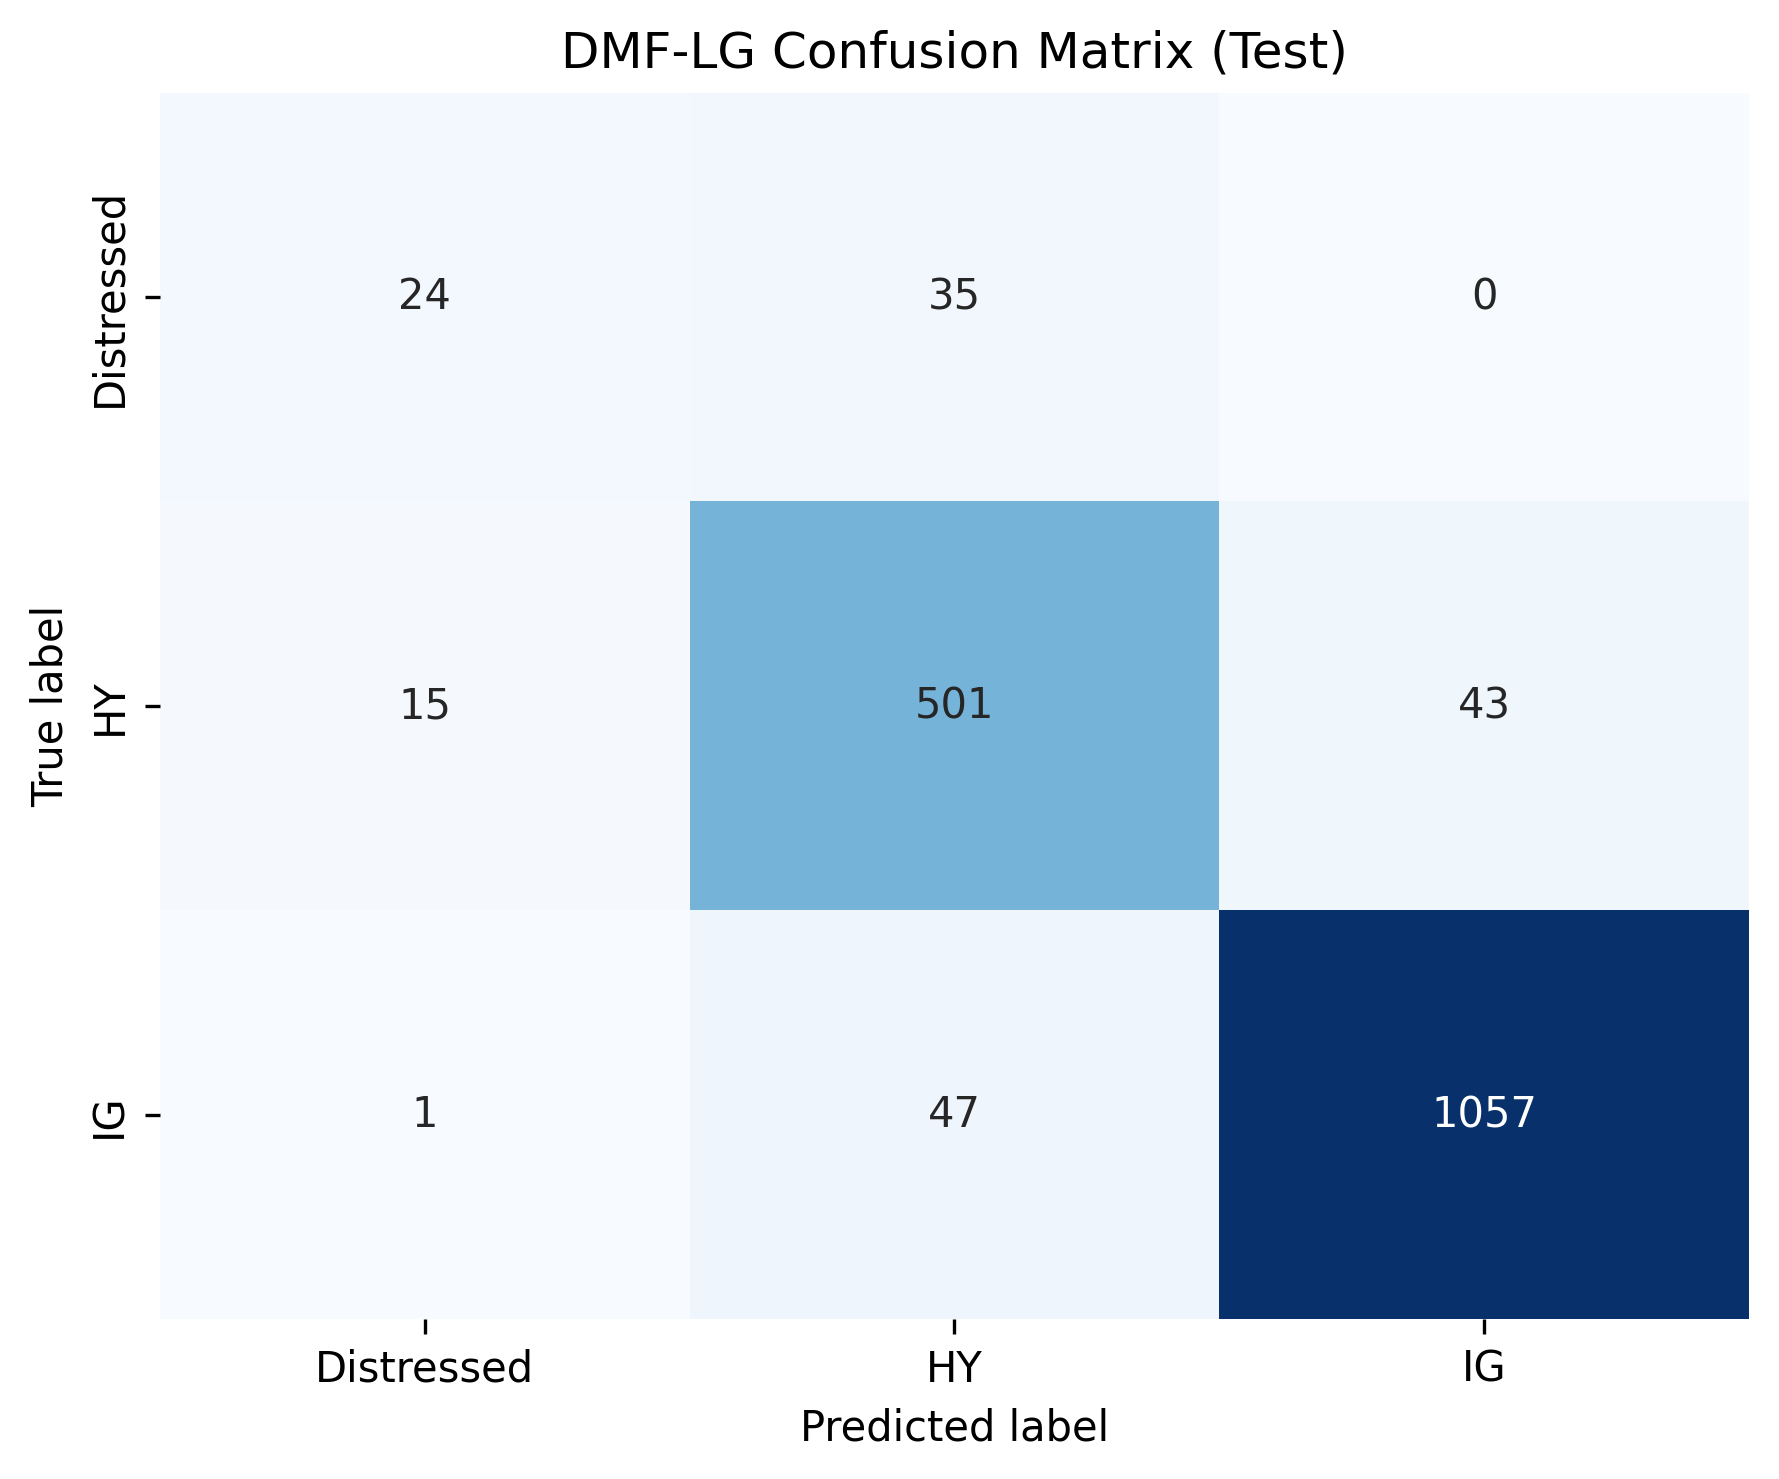
\includegraphics[width=0.95\linewidth]{acc-loss/confusion_dmf_lstm_graphsage.png} & 
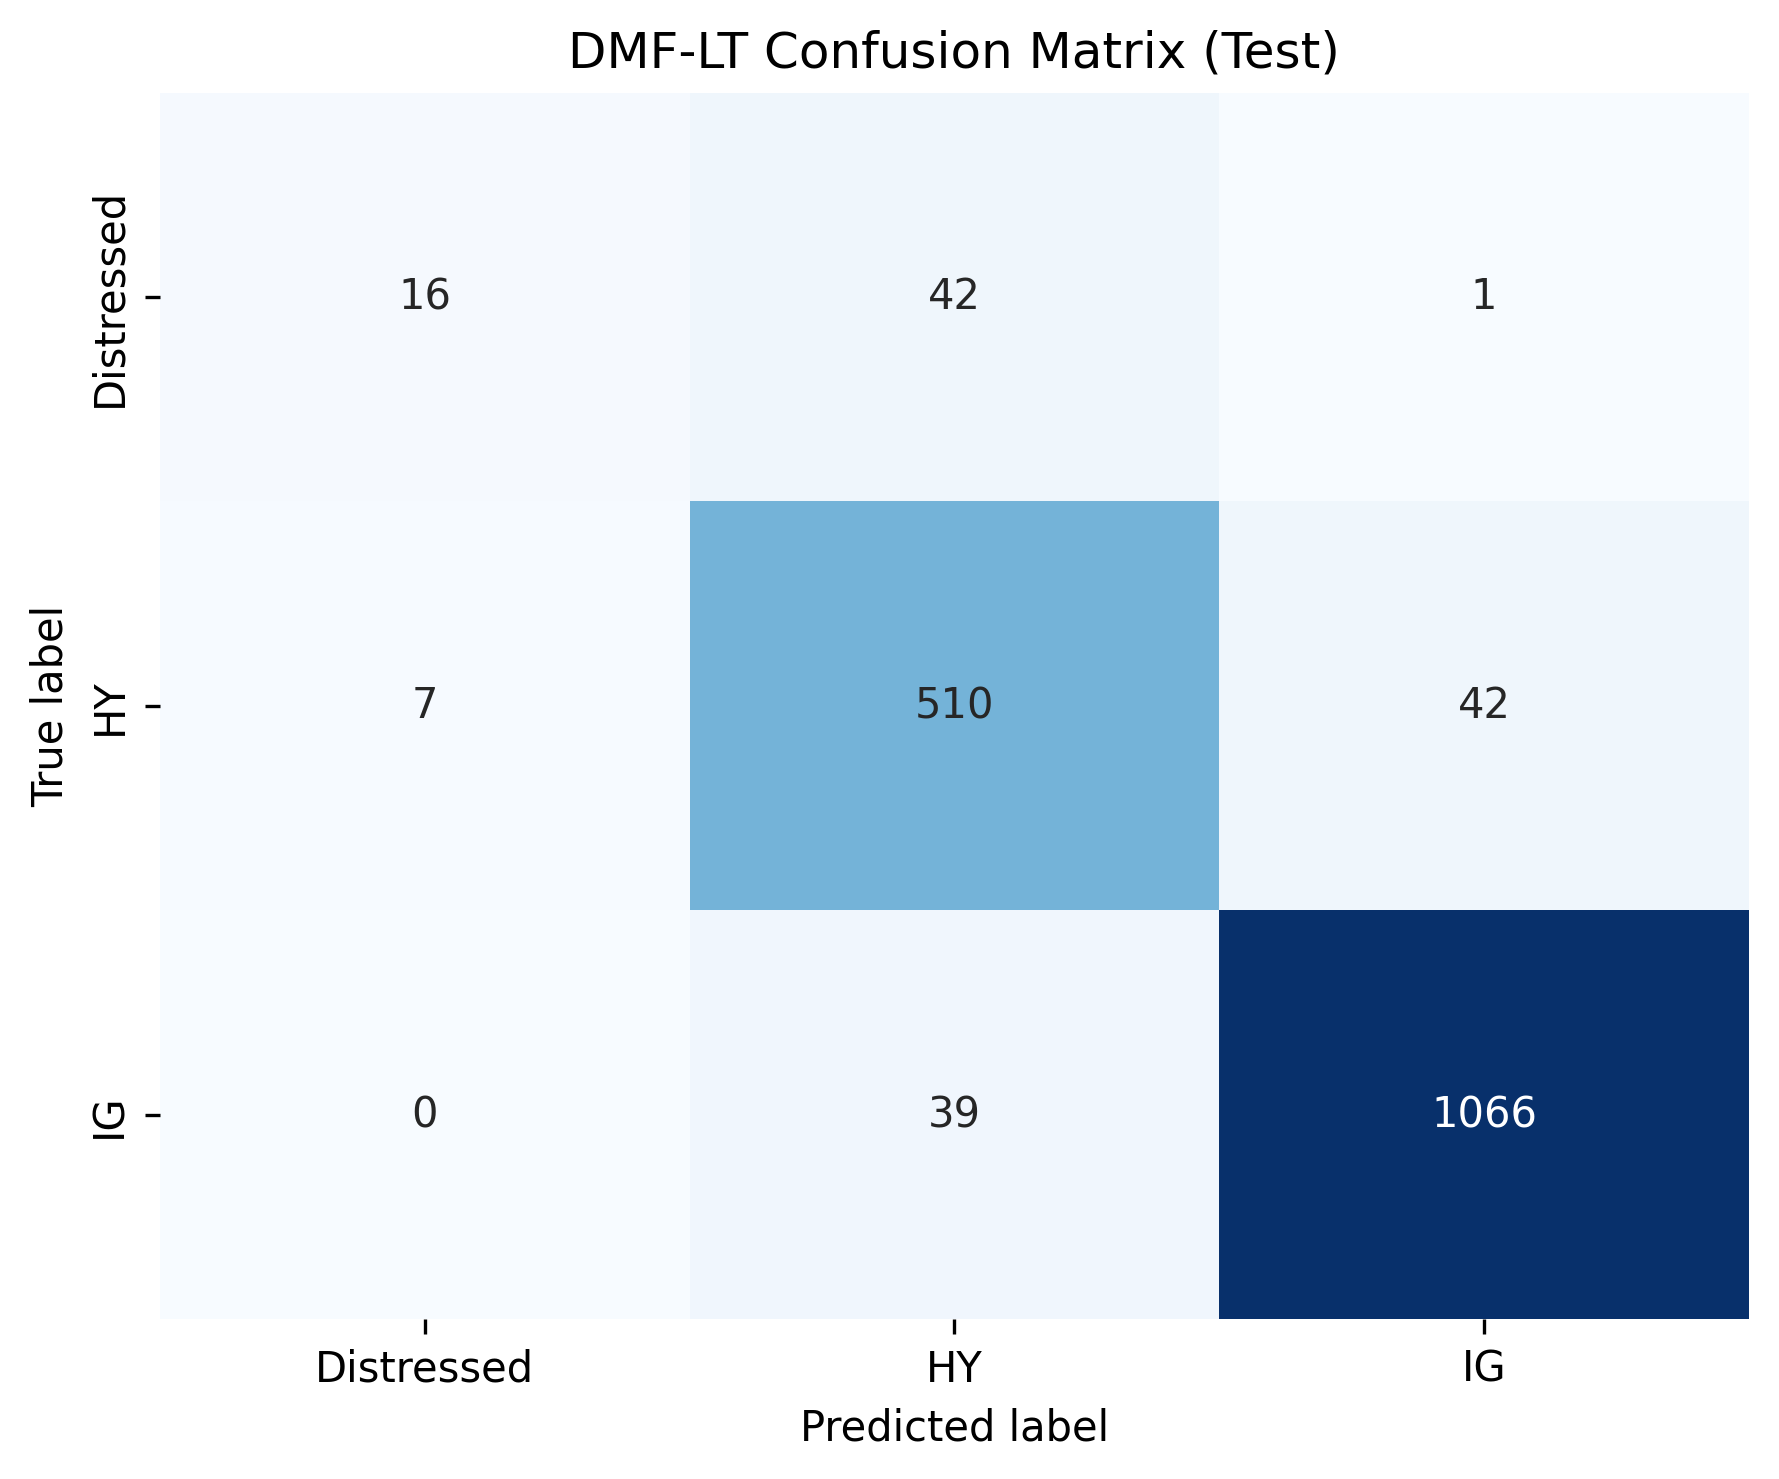
\includegraphics[width=0.95\linewidth]{acc-loss/confusion_dmf_lstm_tlstm.png} \\

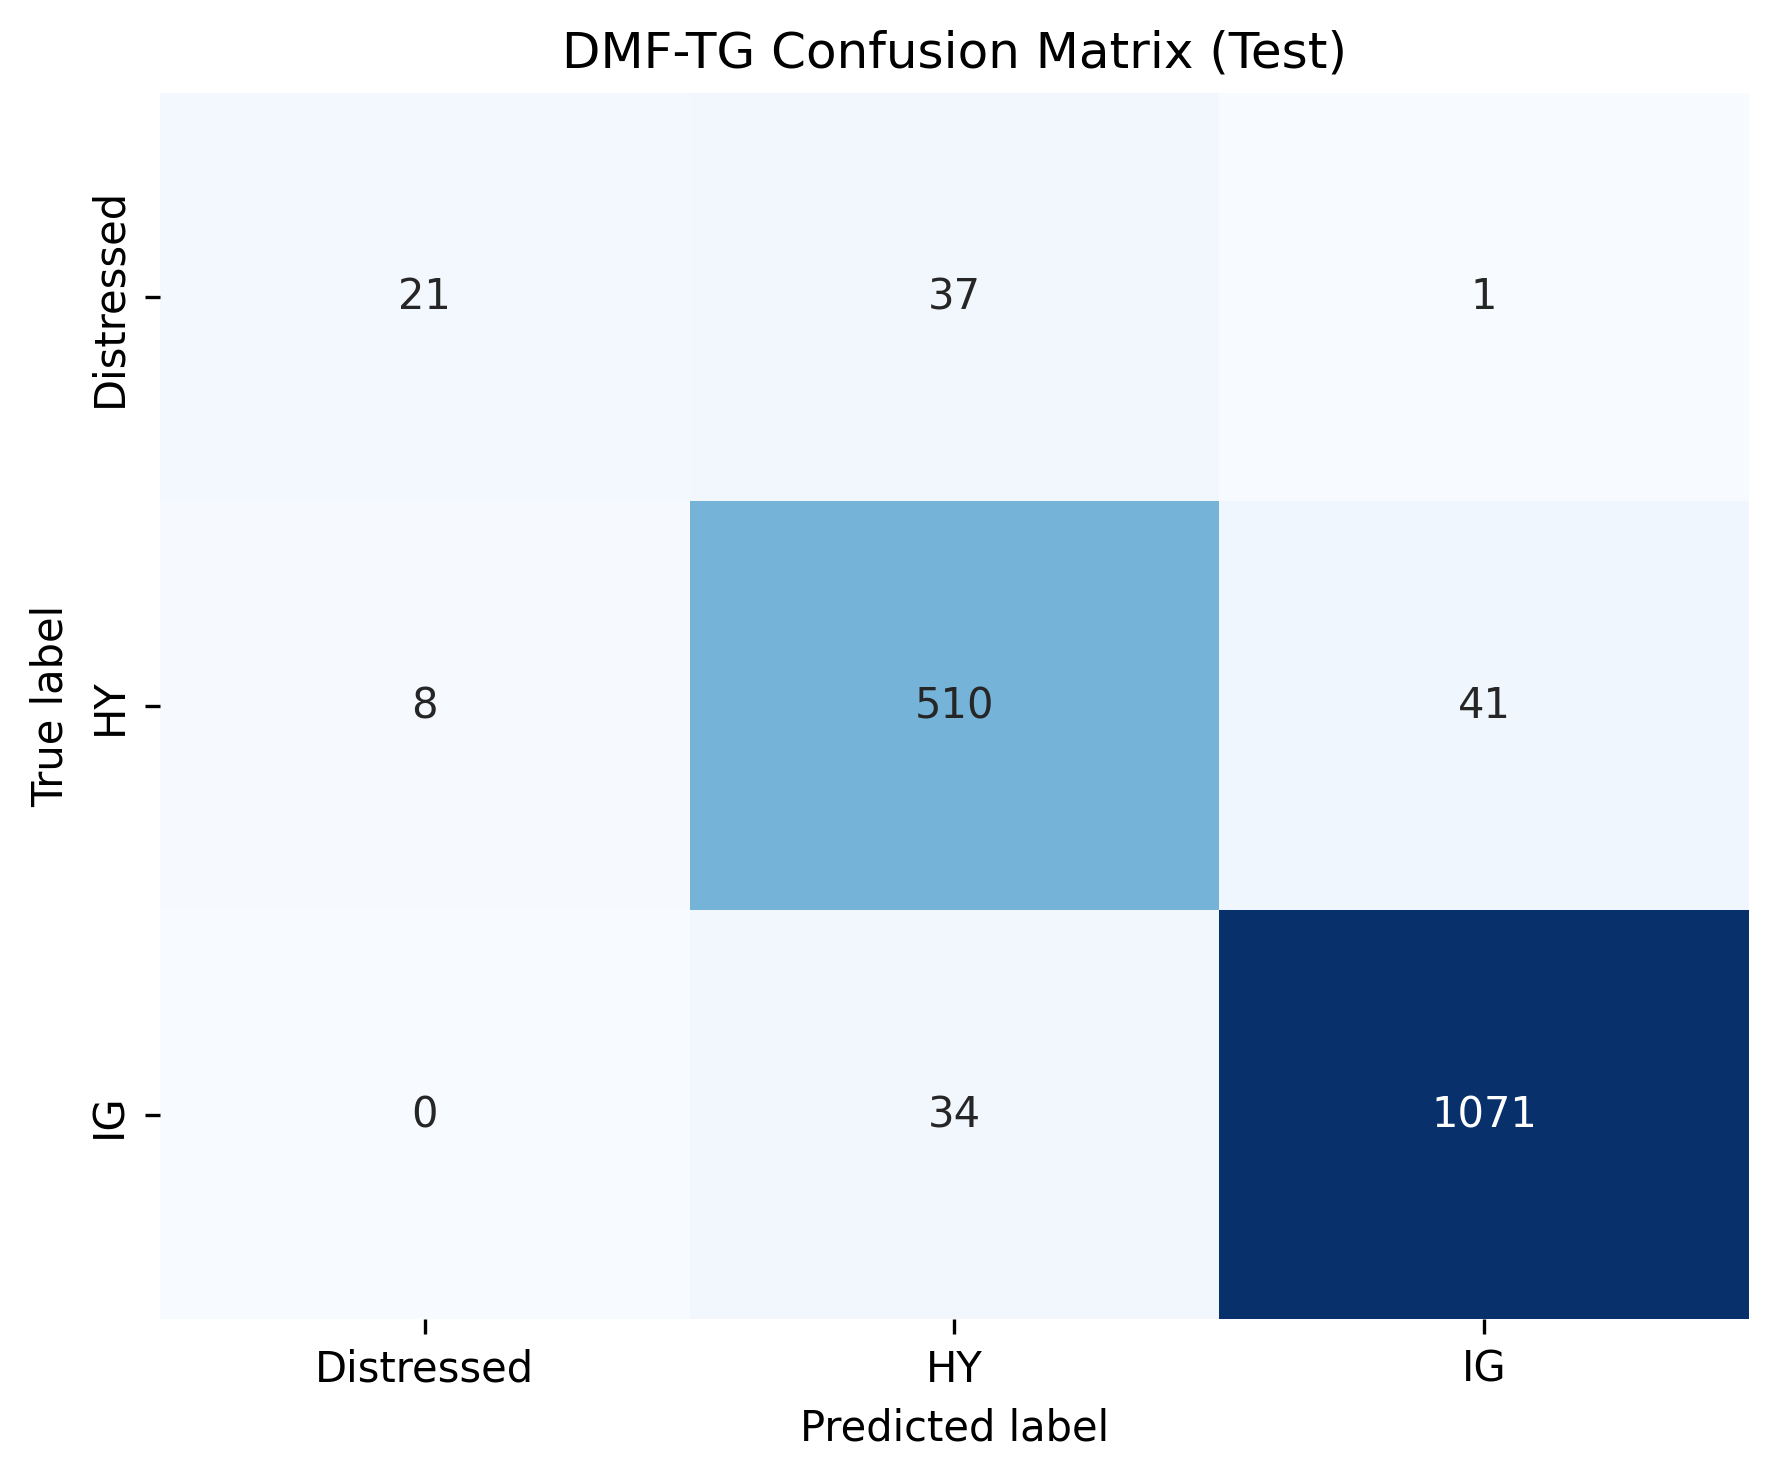
\includegraphics[width=0.95\linewidth]{acc-loss/confusion_dmf_tlstm_graphsage.png} &
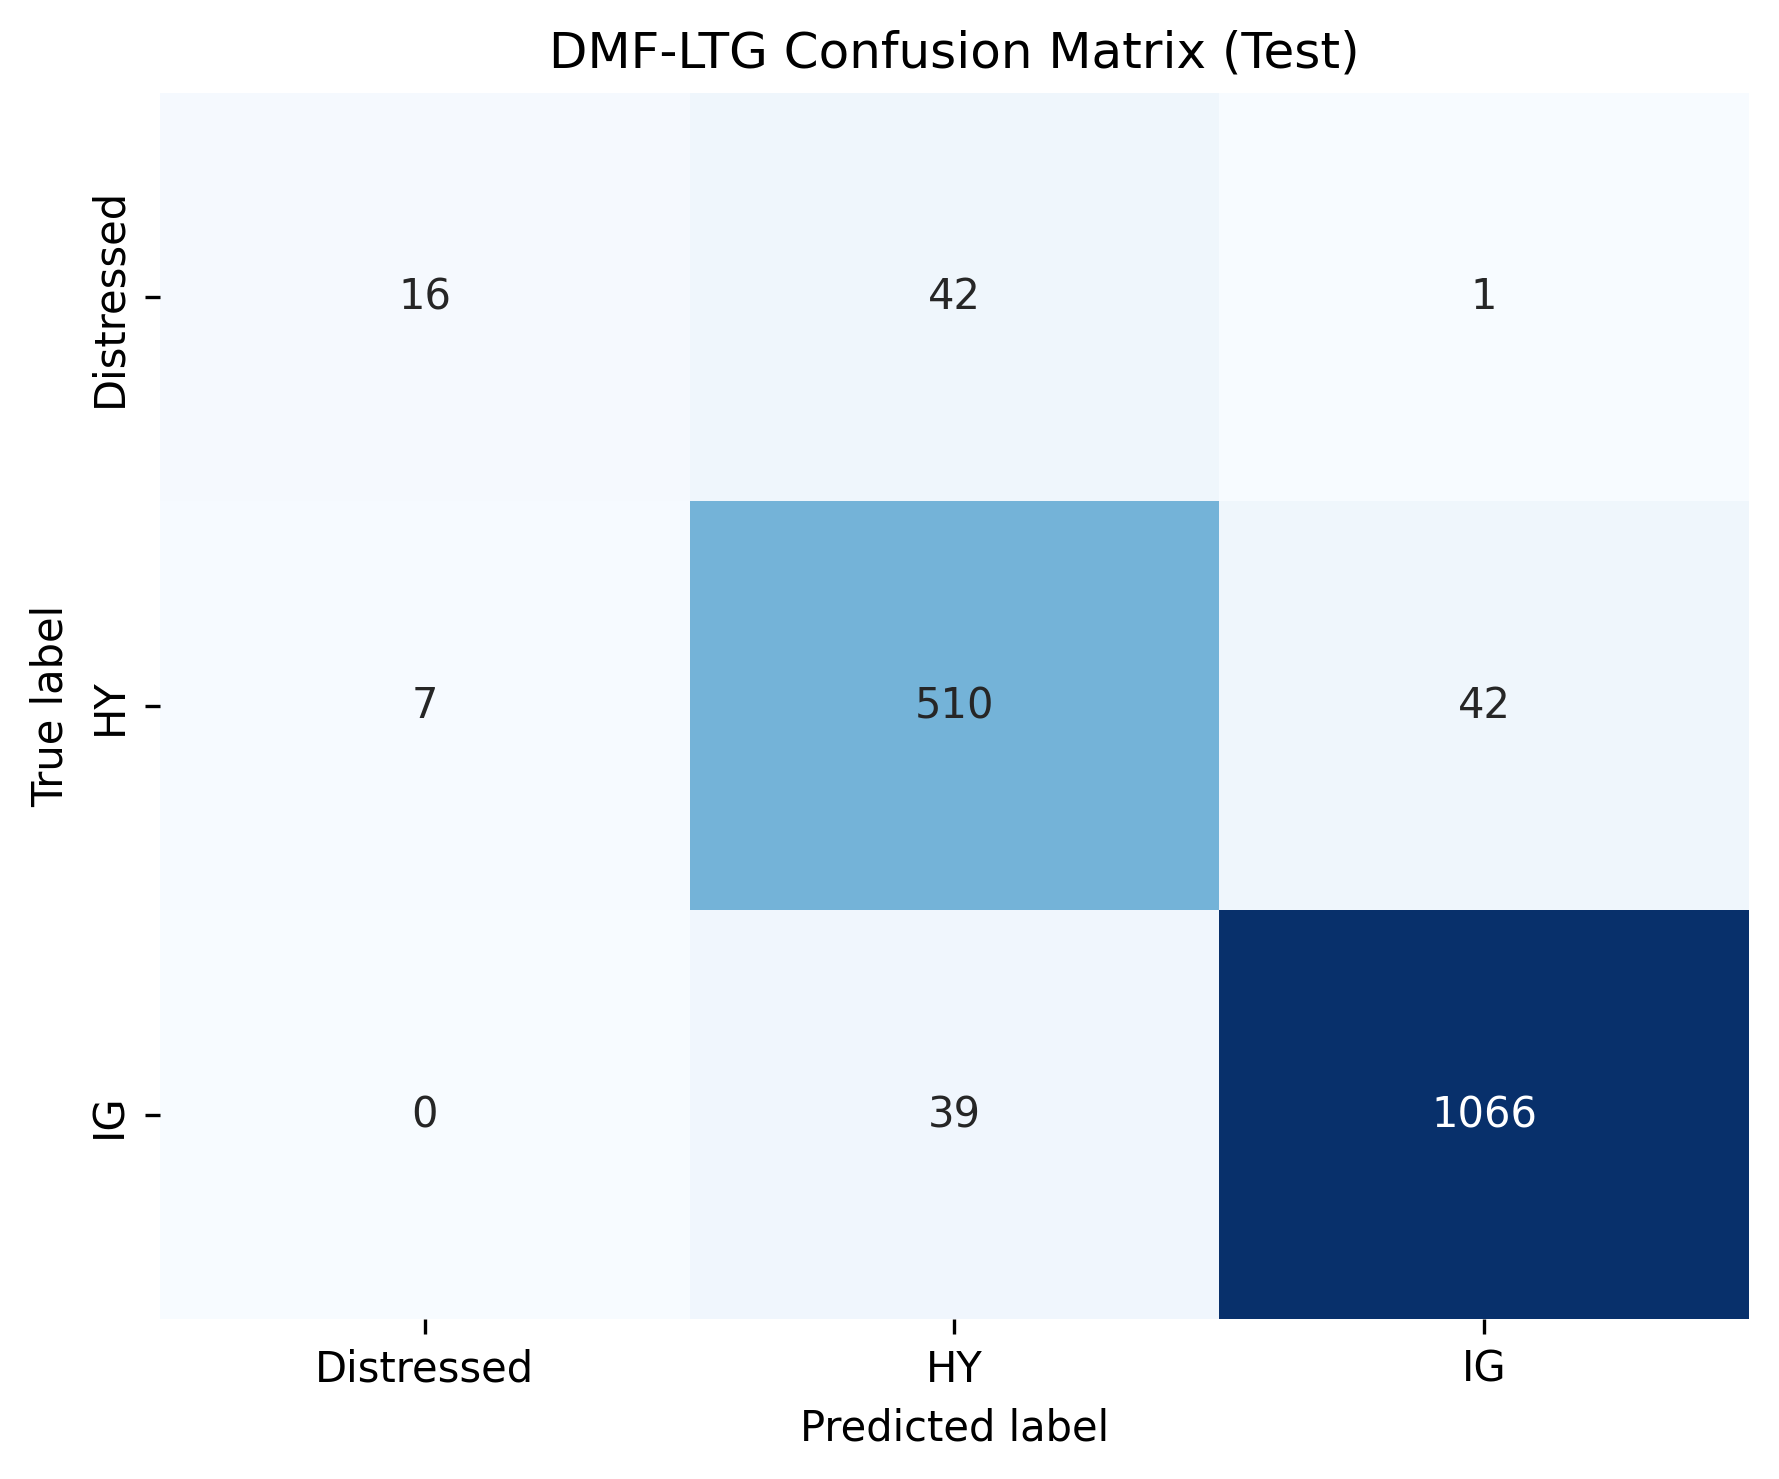
\includegraphics[width=0.95\linewidth]{acc-loss/confusion_dmf_lstm_tlstm_graphsage.png} & \\
\end{longtable}
\endgroup

Từ các ma trận nhầm lẫn trên tập kiểm thử, có thể thấy các mô hình nhìn chung phân loại tốt hai lớp HY và IG.
Trong đó, lớp IG là lớp được nhận diện ổn định nhất, với số lượng mẫu dự đoán đúng cao ở hầu hết các kịch bản.
Điều này cho thấy nhóm doanh nghiệp có chất lượng tín dụng tốt thường có đặc trưng tài chính rõ ràng hơn.
Ngược lại, lớp Distressed là lớp khó nhận diện nhất trong toàn bộ các mô hình.
Lỗi phổ biến nhất là các mẫu Distressed bị dự đoán nhầm sang HY, phản ánh ranh giới giữa hai nhóm này chưa thật sự rõ ràng.
Tuy nhiên, số mẫu Distressed bị nhầm trực tiếp sang IG rất thấp, cho thấy mô hình vẫn phân biệt tốt giữa hai mức rủi ro cách xa nhau.
Trong nhóm mô hình đơn lẻ, GraphSAGE có lợi thế ở lớp Distressed khi dự đoán đúng nhiều mẫu rủi ro cao hơn các mô hình khác.
T-LSTM thể hiện tốt ở lớp IG, cho thấy khả năng học đặc trưng chuỗi thời gian của nhóm doanh nghiệp ổn định.
Các kịch bản Fuzzy Ensemble giúp duy trì kết quả ổn định ở hai lớp HY và IG nhưng chưa cải thiện rõ rệt lớp Distressed.
Trong nhóm DMF, DMF-TG là kịch bản nổi bật nhất khi đạt số lượng mẫu IG dự đoán đúng cao nhất và hiệu quả tổng thể tốt.
Nhóm DMF cho thấy ưu thế trong việc nâng cao độ chính xác tổng thể, đặc biệt ở hai lớp HY và IG.
Tuy nhiên, nếu mục tiêu là phát hiện sớm doanh nghiệp rủi ro cao, cần tiếp tục cải thiện khả năng nhận diện lớp Distressed.

\subsubsection{Precision của các kịch bản}

\begin{figure}[H]
\centering
\setupfairsubfigures
\begin{subfigure}{\fairfigurewidth}
    \centering
    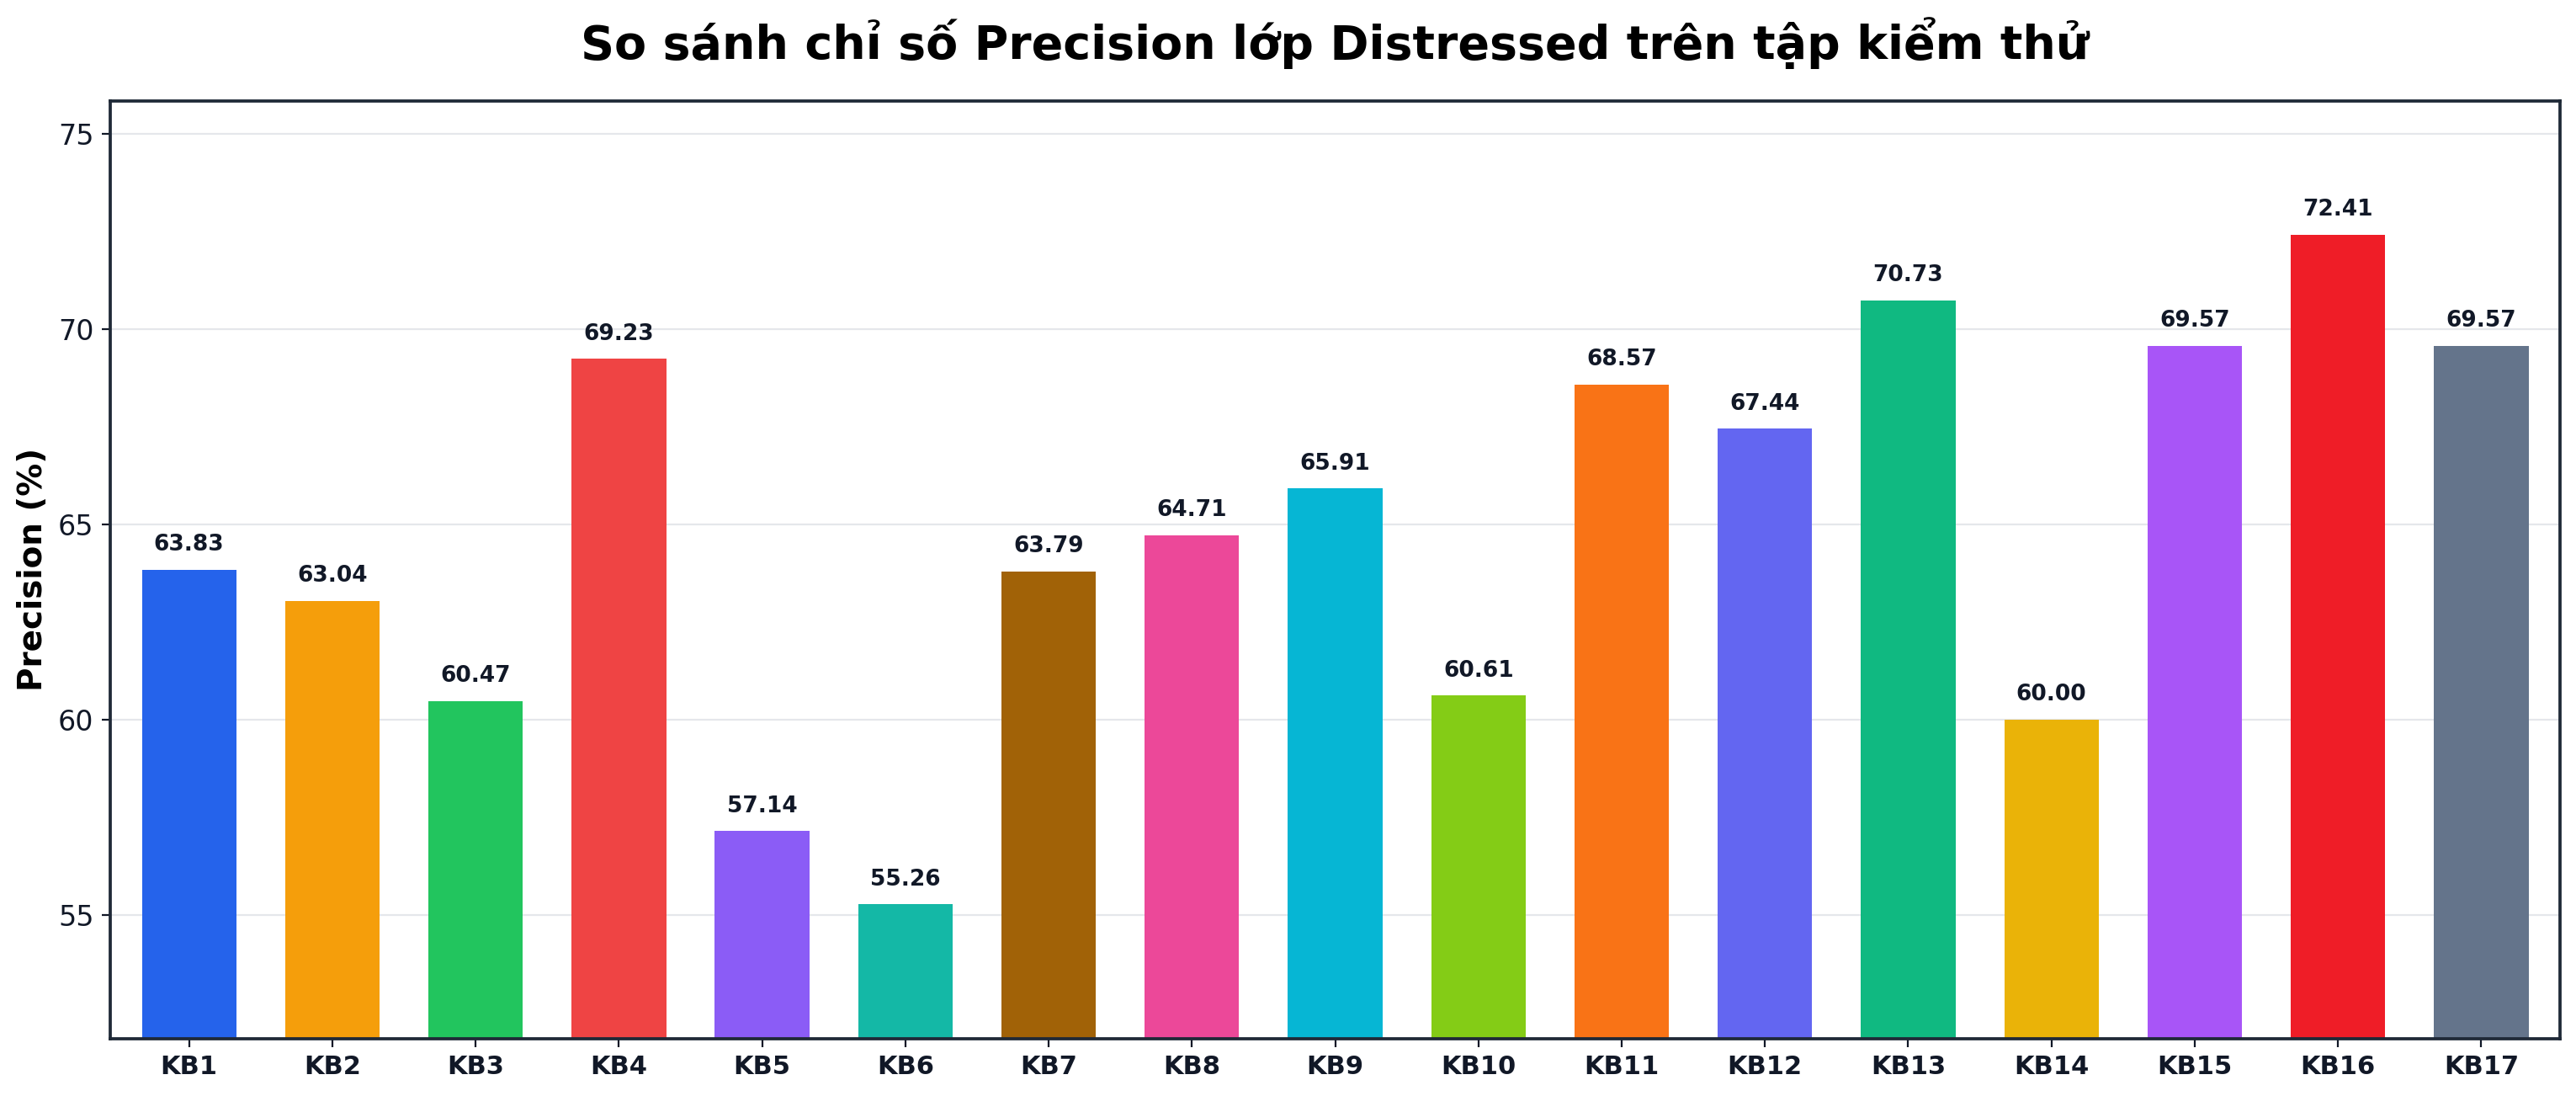
\includegraphics[width=\textwidth]{acc-loss/metric_precision_distressed_test.png}
    \caption{Precision của lớp Distressed}
    \label{fig:precision_distressed}
\end{subfigure}
\end{figure}

\begin{figure}[H]
\ContinuedFloat
\centering
\begin{subfigure}{\fairfigurewidth}
    \centering
    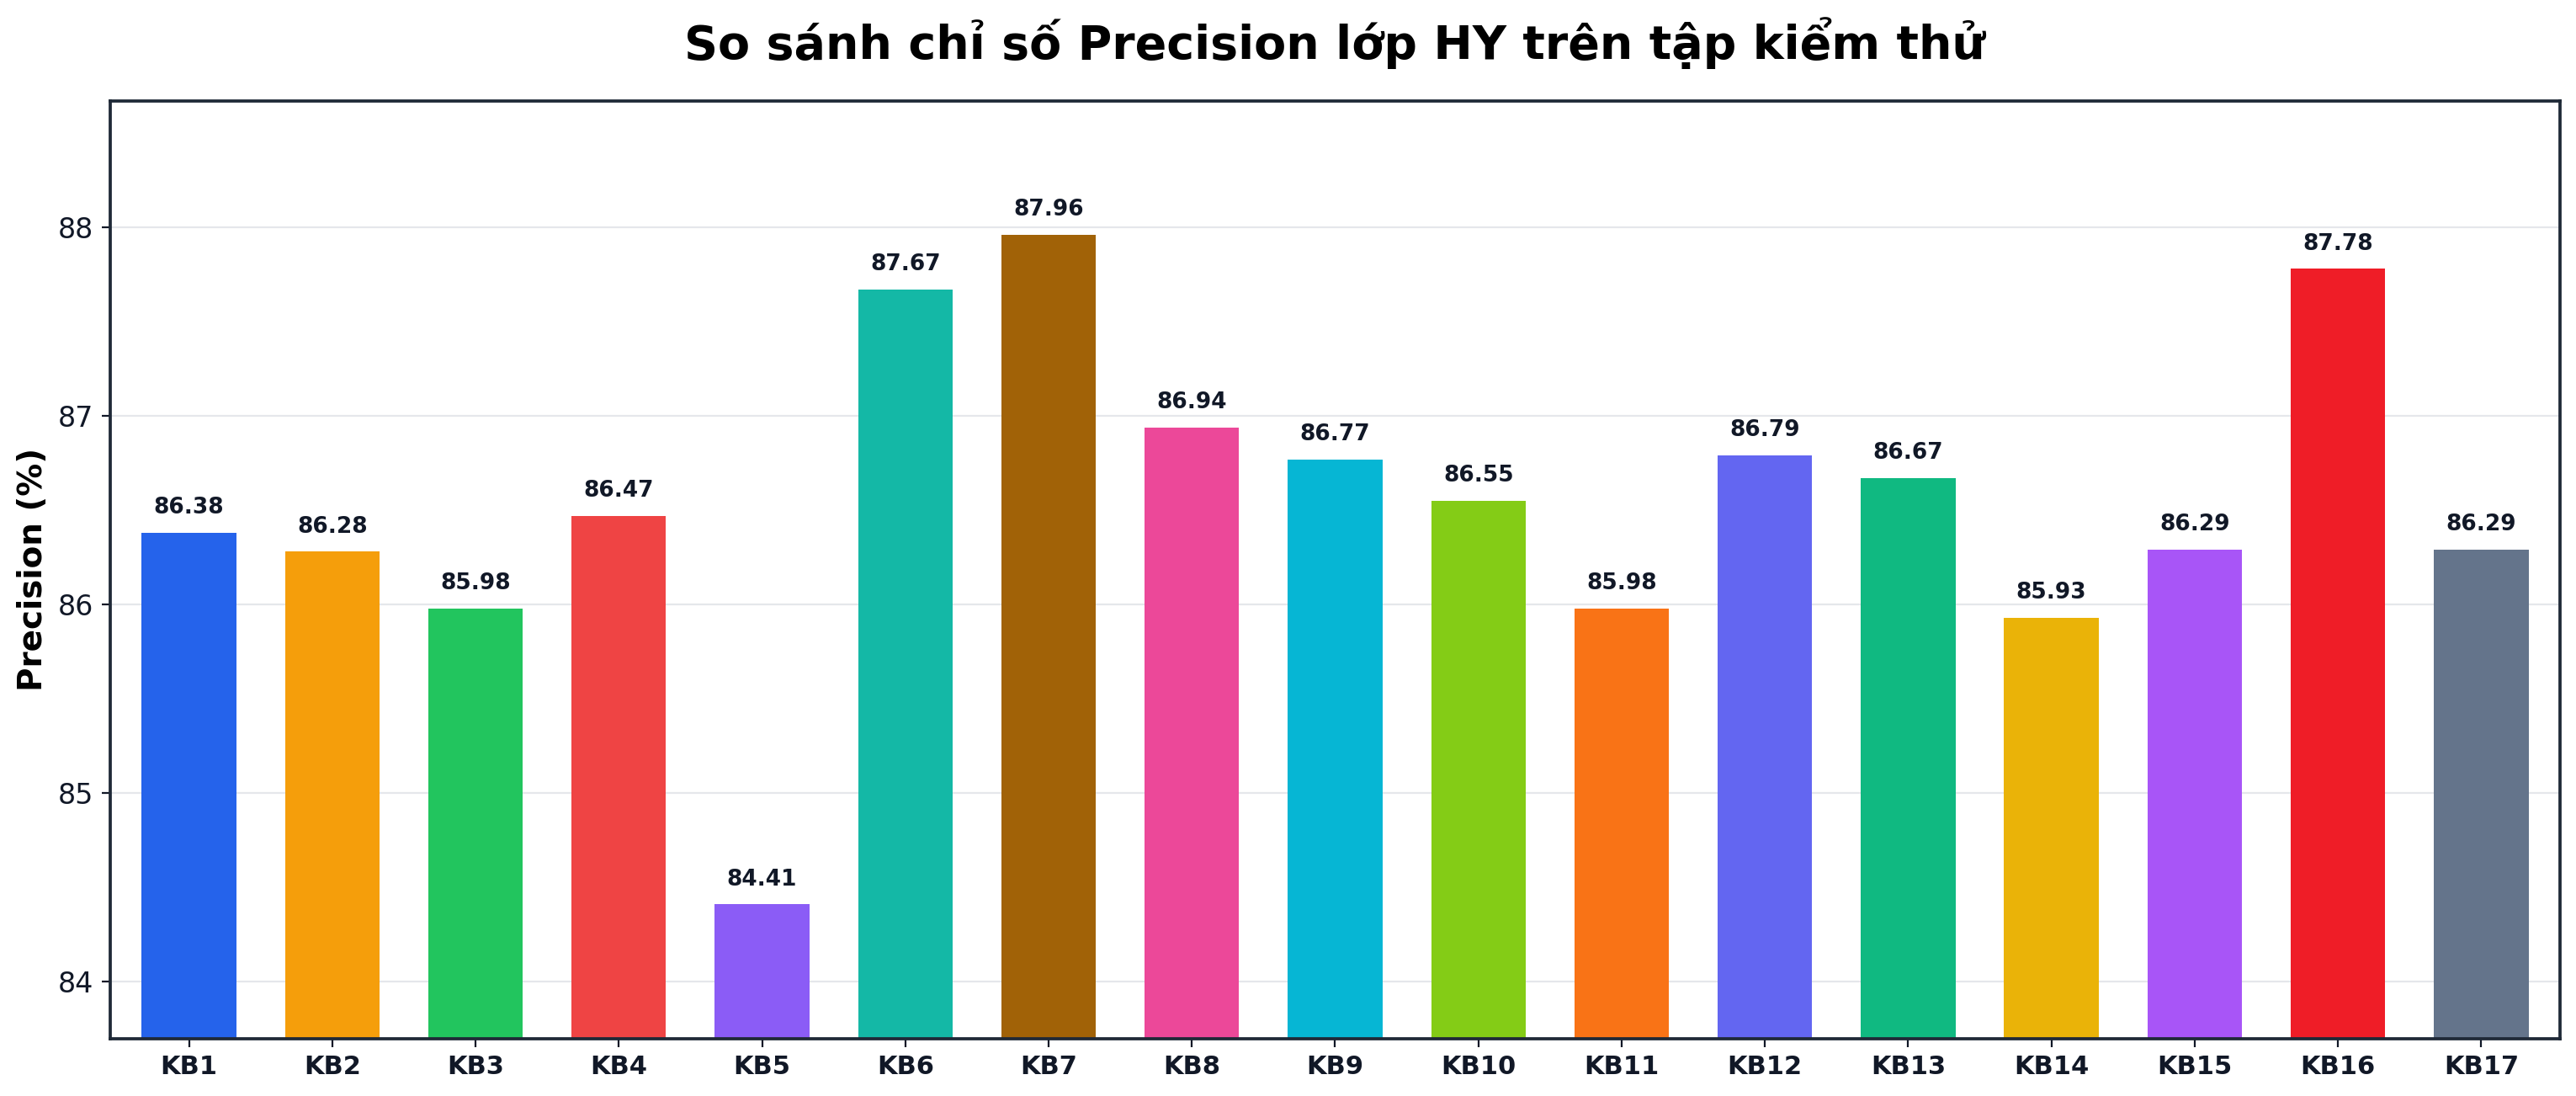
\includegraphics[width=\textwidth]{acc-loss/metric_precision_hy_test.png}
    \caption{Precision của lớp HY (High Yield)}
    \label{fig:precision_hy}
\end{subfigure}

\end{figure}

\begin{figure}[H]
\ContinuedFloat
\centering
\begin{subfigure}{\fairfigurewidth}
    \centering
    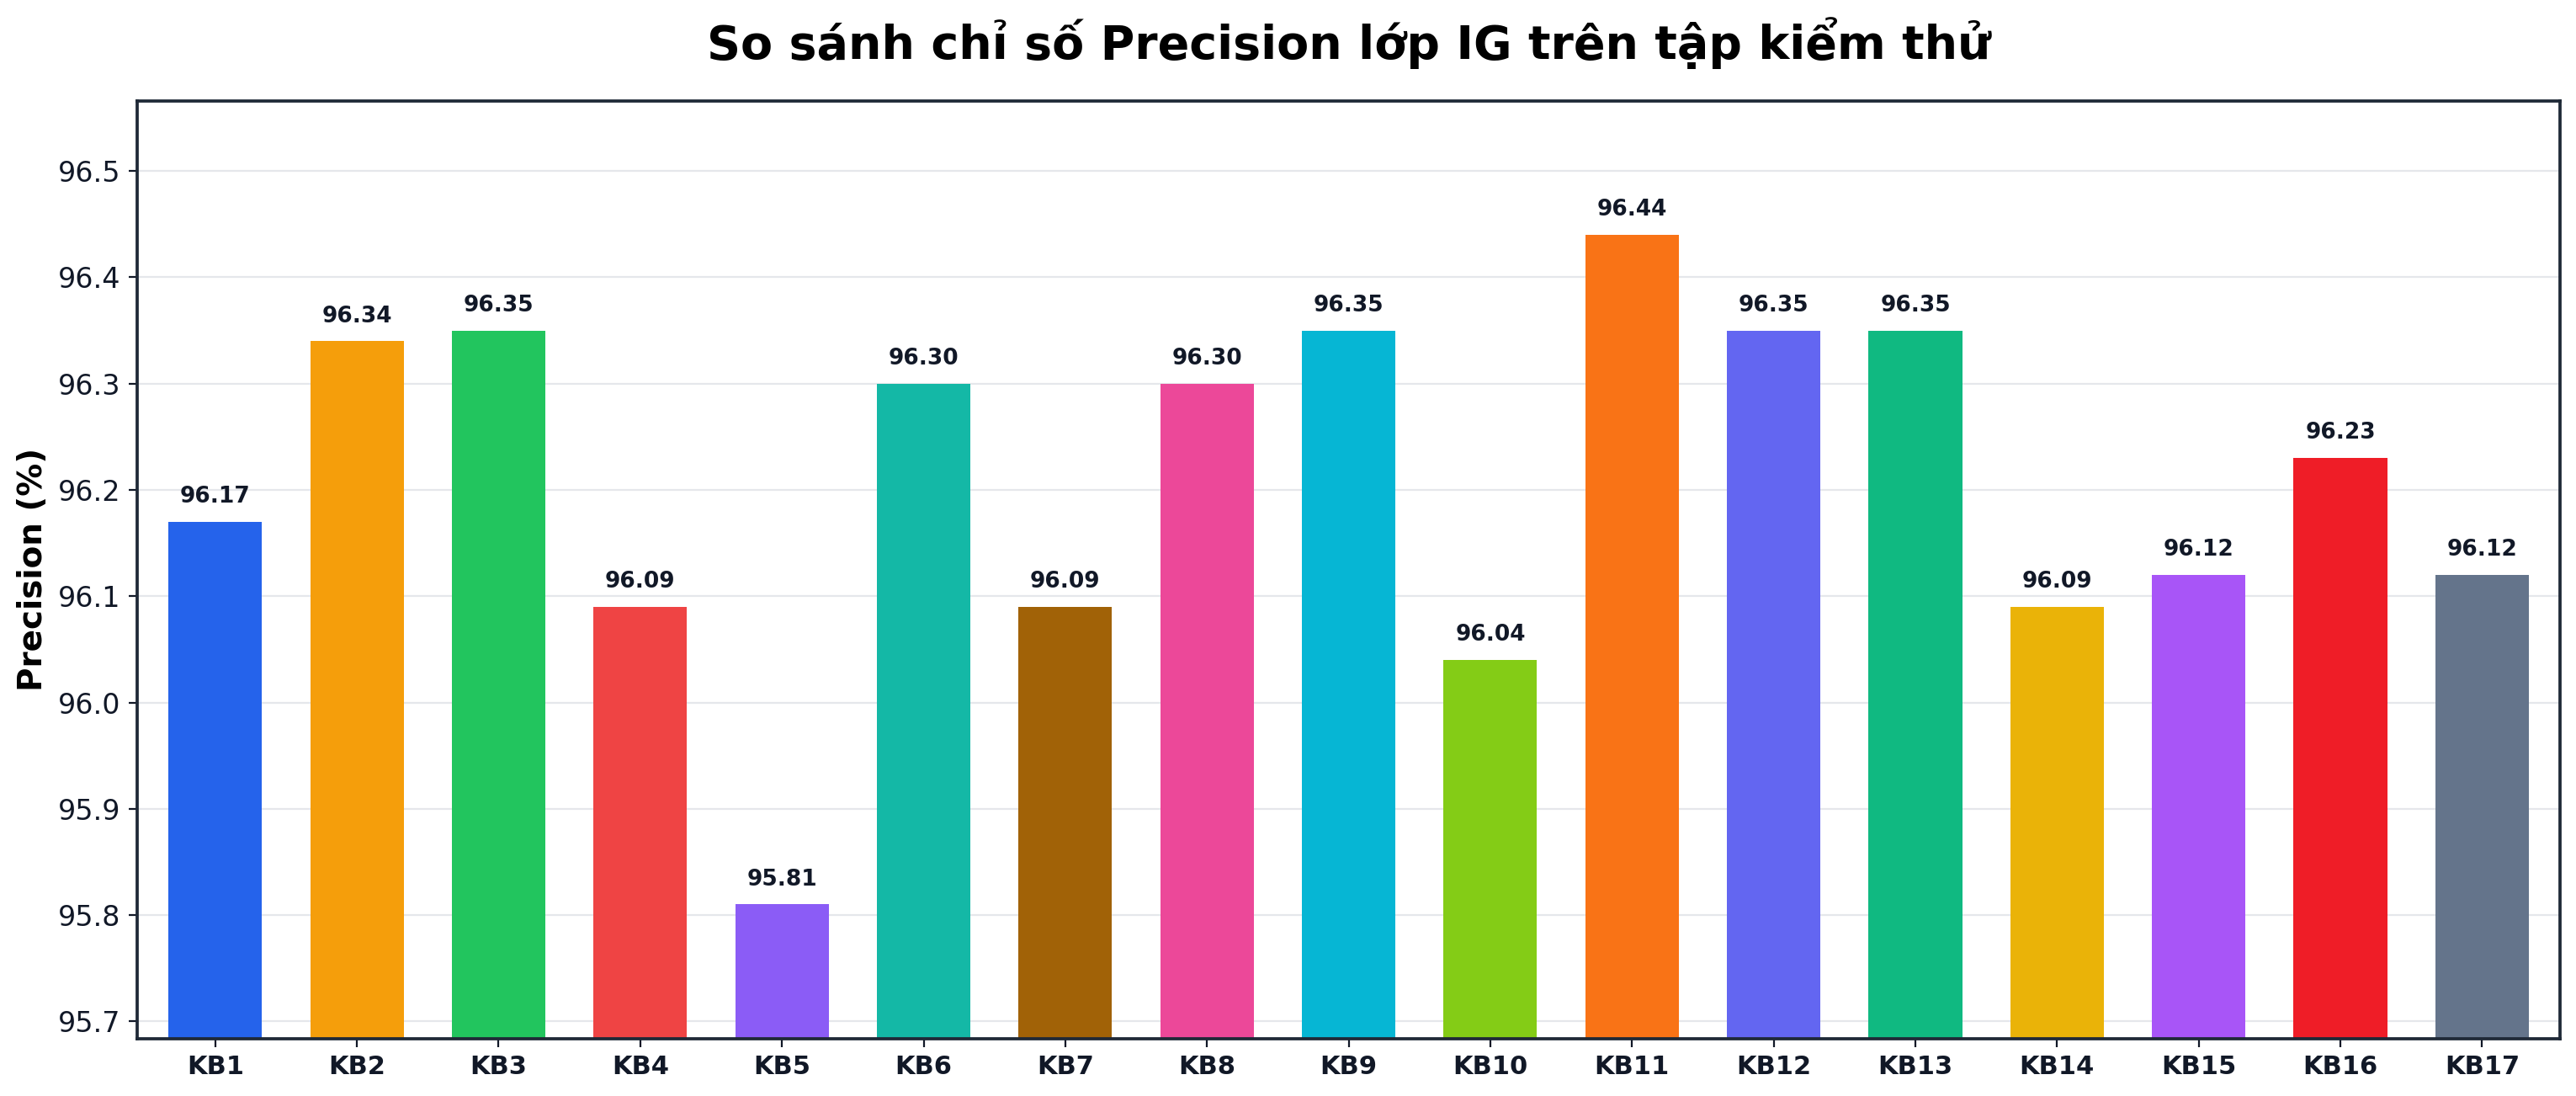
\includegraphics[width=\textwidth]{acc-loss/metric_precision_ig_test.png}
    \caption{Precision của lớp IG (Investment Grade)}
    \label{fig:precision_ig}
\end{subfigure}
\caption{Precision lớp Distressed (a), lớp HY (b) và lớp IG (c) trên tập kiểm thử}
\label{fig:precision_classes}
\end{figure}

Kết quả Precision trên tập kiểm thử cho thấy hiệu quả dự đoán của các mô hình có sự khác biệt giữa ba lớp xếp hạng tín dụng.
Trong đó, lớp IG đạt Precision cao và ổn định nhất, chủ yếu quanh mức 96\%, cho thấy khả năng nhận diện tốt nhóm doanh nghiệp có chất lượng tín dụng cao.
Lớp HY cũng có kết quả tương đối đồng đều, dao động trong khoảng 84,41\%–87,96\%. GraphSAGE đạt Precision cao nhất ở lớp HY với 87,96\%, tiếp theo là DMF-TG và T-LSTM. Ngược lại, lớp Distressed là lớp khó phân loại nhất do số lượng mẫu ít và ranh giới với lớp HY chưa rõ ràng.
Trong nhóm mô hình đơn lẻ, LSTM đạt Precision cao nhất cho lớp Distressed với 69,23\%. Ở nhóm Fuzzy Ensemble, FR-TTLPXL đạt kết quả tốt nhất cho lớp Distressed với 70,73\%. Đáng chú ý, DMF-TG đạt Precision lớp Distressed cao nhất toàn bộ biểu đồ với 72,41\%. Điều này cho thấy việc kết hợp động giữa T-LSTM và GraphSAGE giúp cải thiện khả năng nhận diện doanh nghiệp rủi ro cao. Nhìn chung, DMF-TG là kịch bản nổi bật nhất khi vừa nâng cao Precision ở lớp Distressed, vừa duy trì hiệu quả tốt ở hai lớp HY và IG.

\subsubsection{Recall của các kịch bản}
\begin{figure}[H]
\centering
\setupfairsubfigures
\begin{subfigure}{\fairfigurewidth}
    \centering
    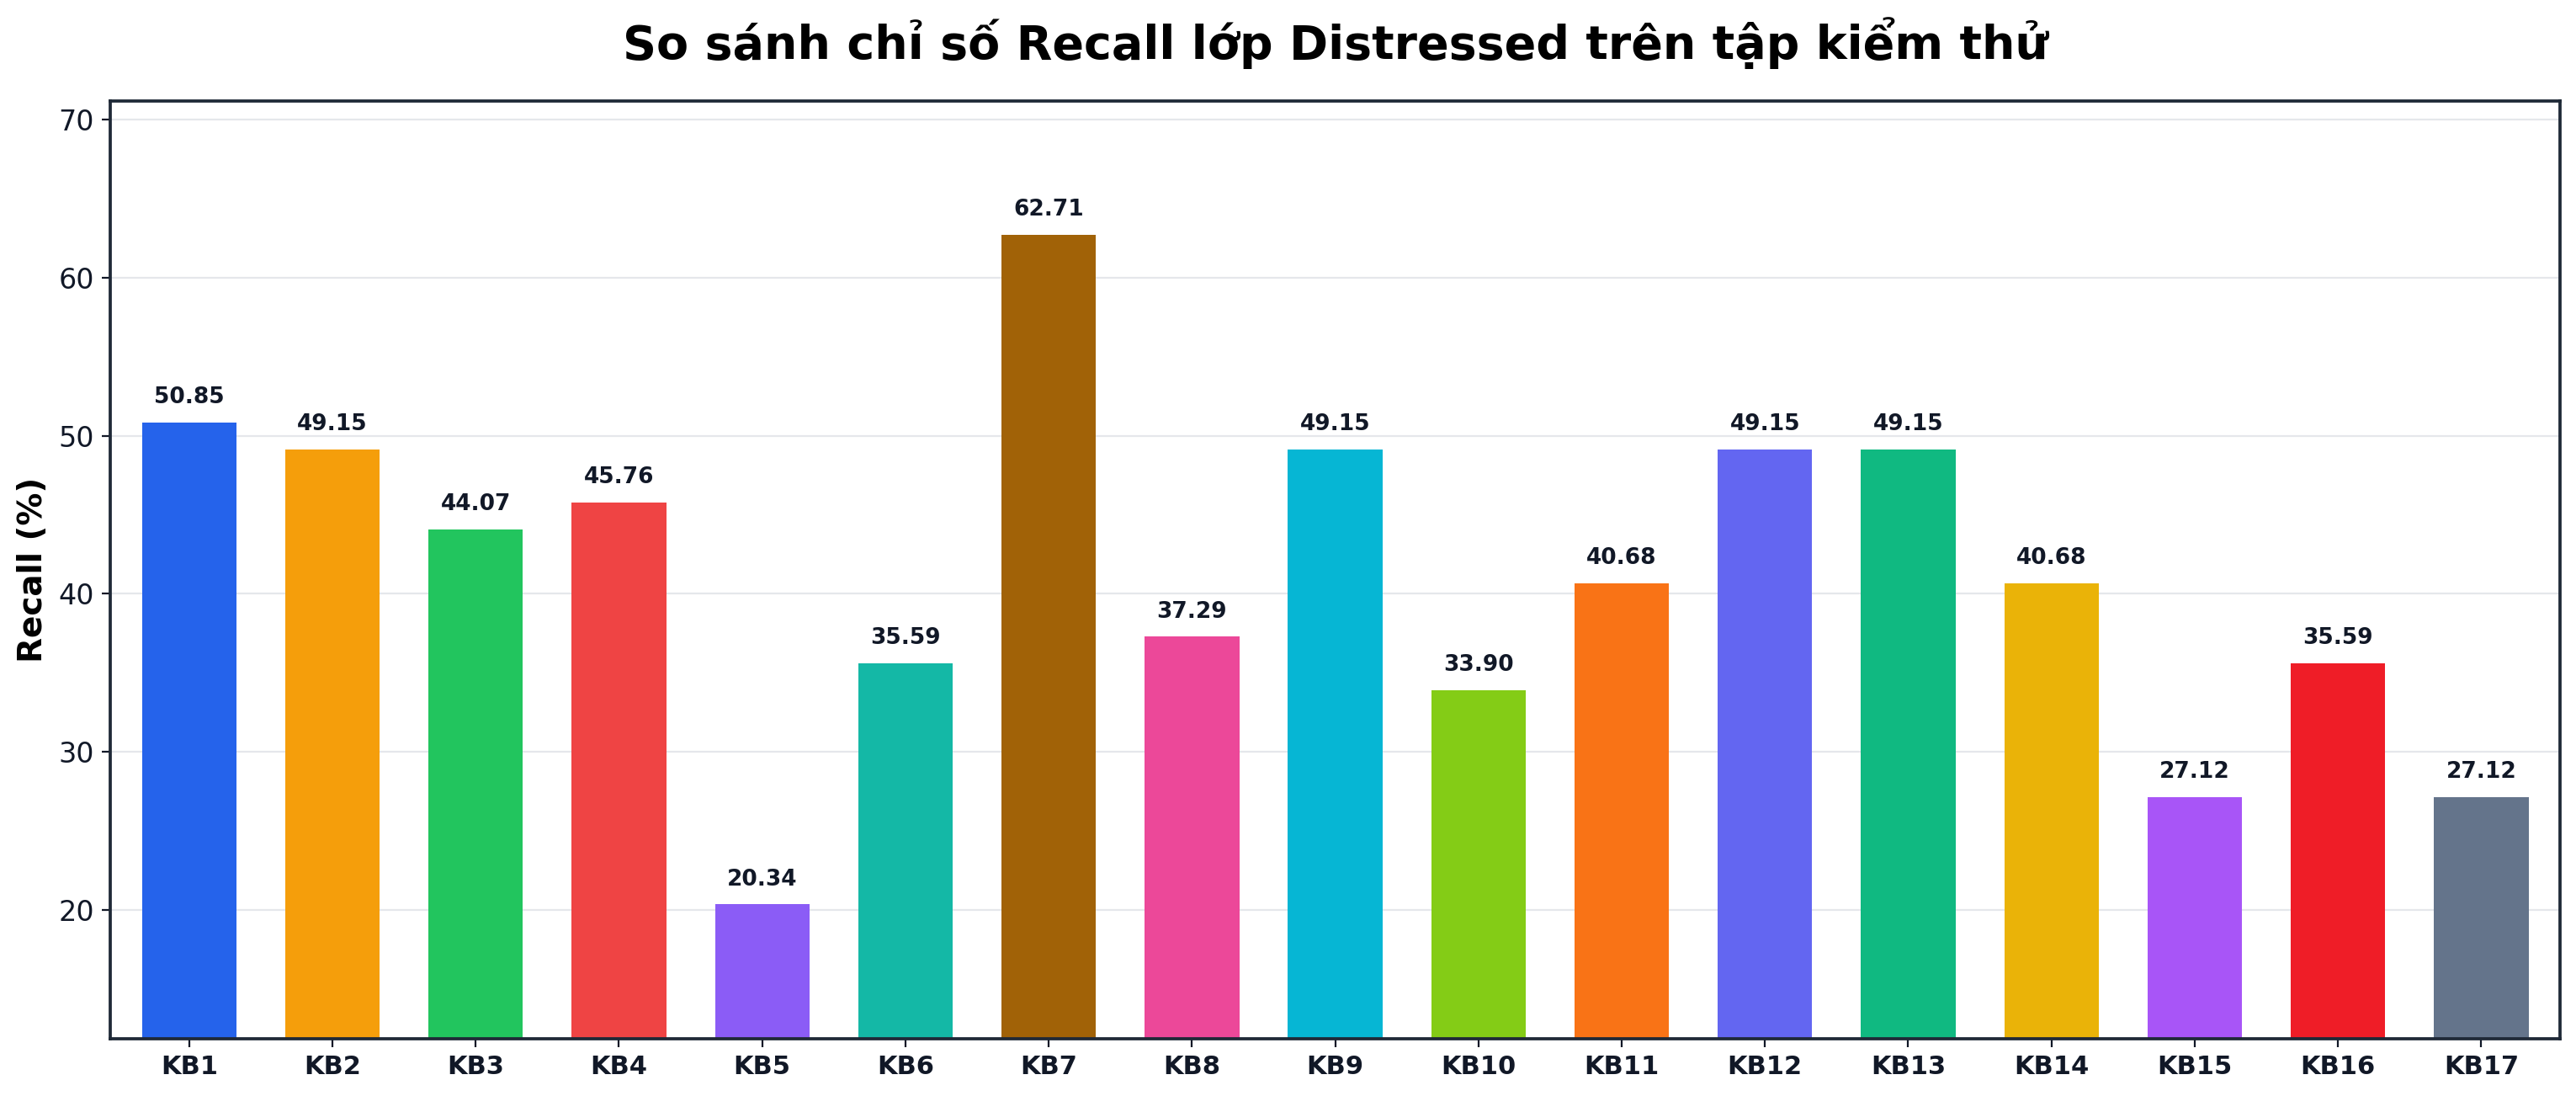
\includegraphics[width=\textwidth]{acc-loss/metric_recall_distressed_test.png}
    \caption{Recall của lớp Distressed}
    \label{fig:Recall_distressed}
\end{subfigure}
\end{figure}

\begin{figure}[H]
\ContinuedFloat
\centering
\begin{subfigure}{\fairfigurewidth}
    \centering
    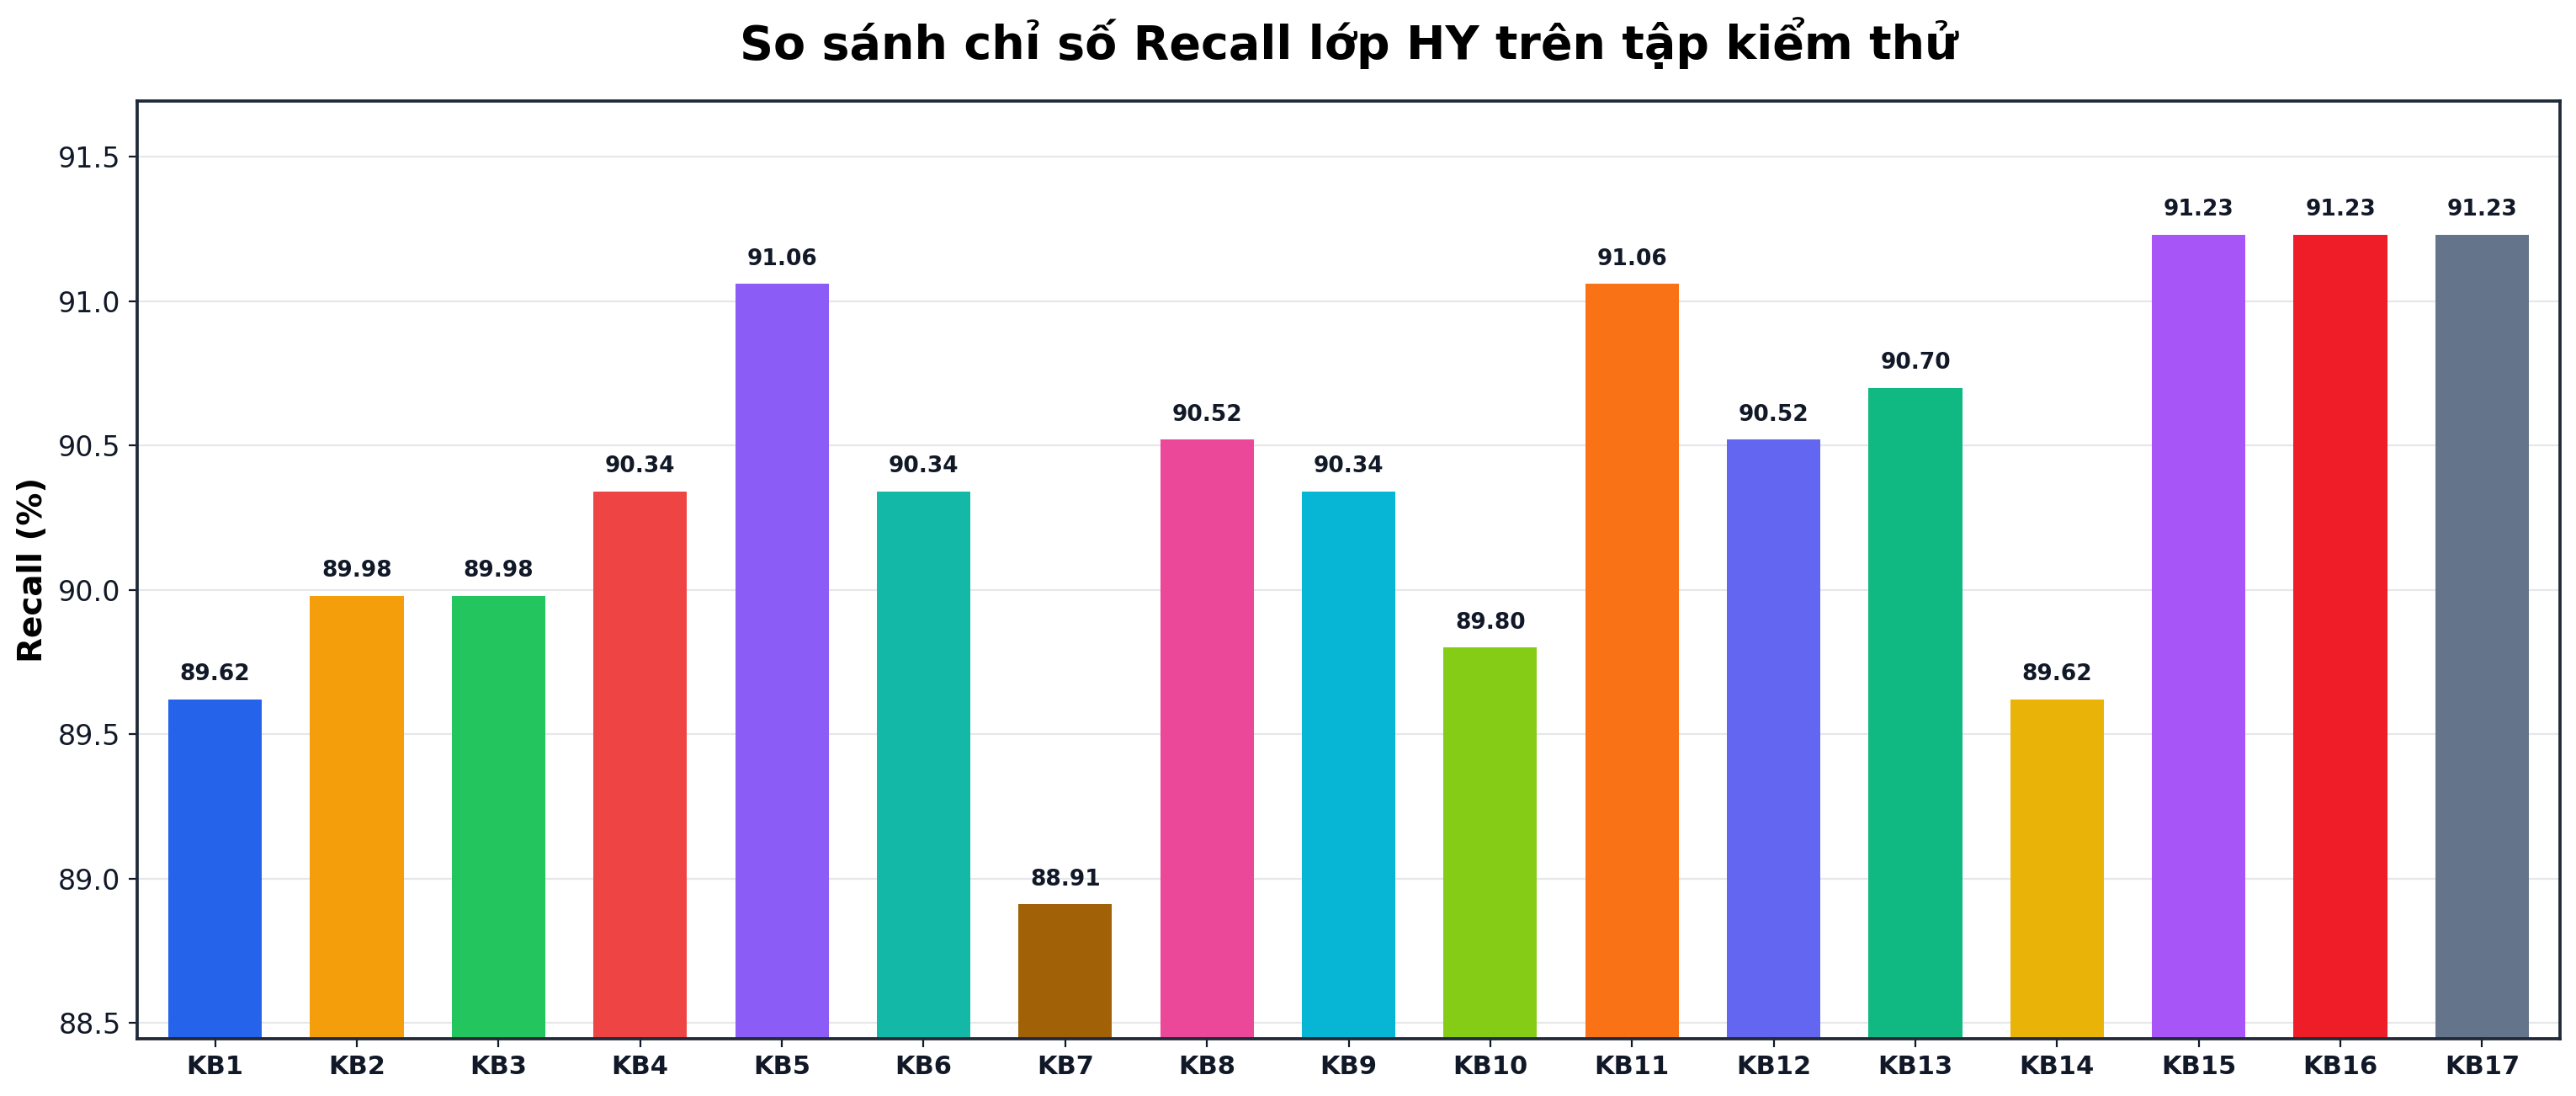
\includegraphics[width=\textwidth]{acc-loss/metric_recall_hy_test.png}
    \caption{Recall của lớp HY (High Yield)}
    \label{fig:Recall_hy}
\end{subfigure}
\end{figure}

\begin{figure}[H]
\ContinuedFloat
\centering
\begin{subfigure}{\fairfigurewidth}
    \centering
    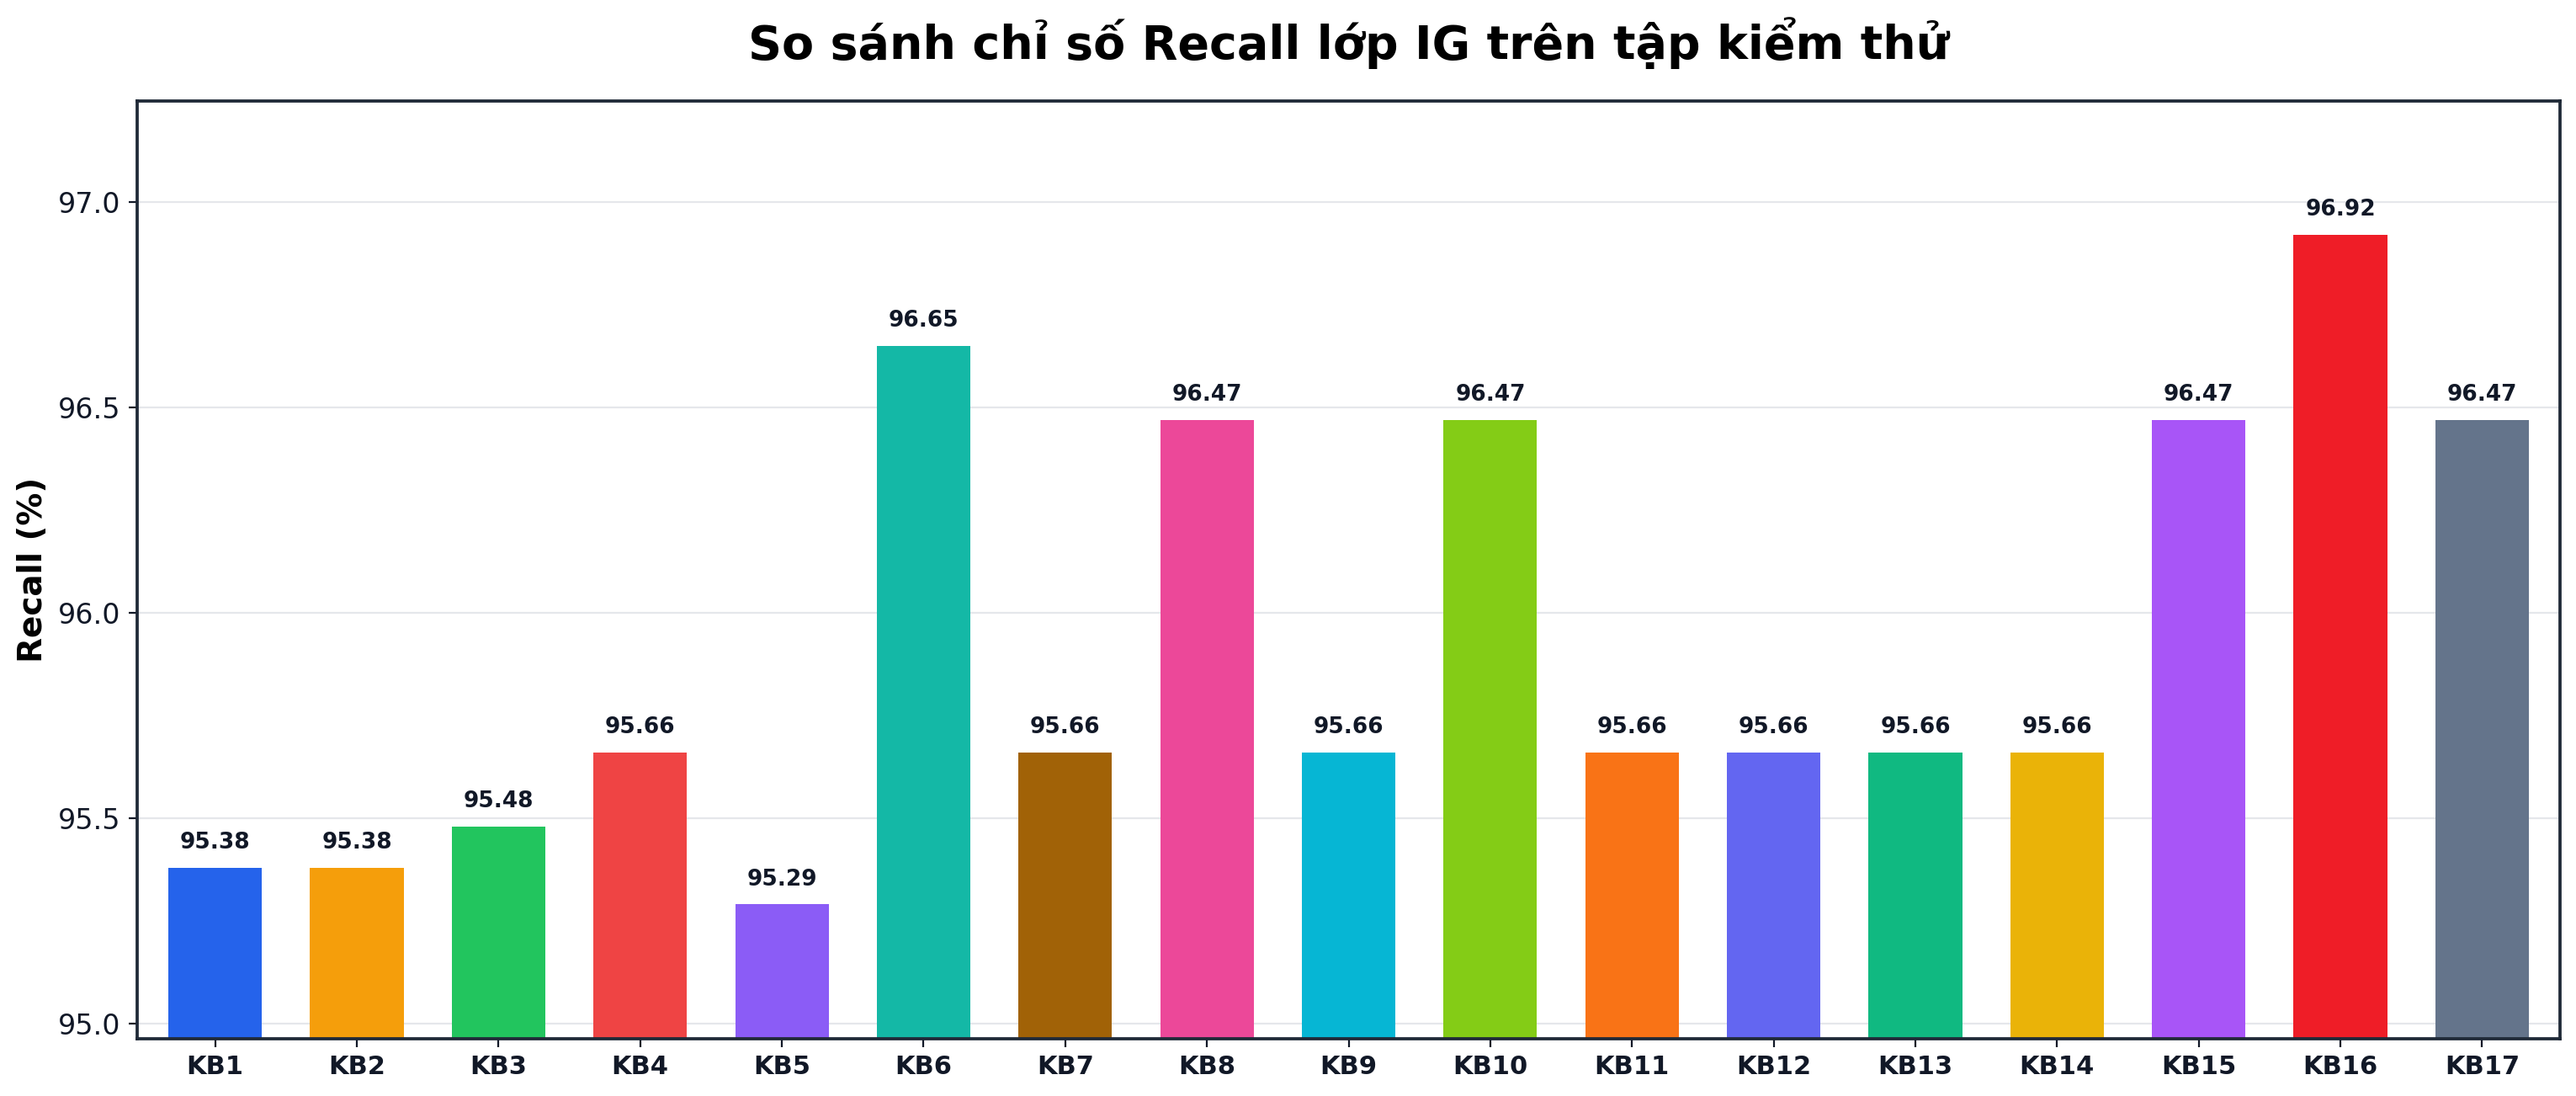
\includegraphics[width=\textwidth]{acc-loss/metric_recall_ig_test.png}
    \caption{Recall của lớp IG (Investment Grade)}
    \label{fig:Recall_ig}
\end{subfigure}
\caption{Recall lớp Distressed (a), lớp HY (b) và lớp IG (c) trên tập kiểm thử}
\label{fig:Recall_classes}
\end{figure}
Chỉ số Recall cho thấy khả năng nhận diện đầy đủ các mẫu thuộc từng lớp xếp hạng tín dụng.
Kết quả cho thấy lớp Distressed là lớp khó nhận diện nhất và có mức dao động lớn giữa các mô hình.
GraphSAGE đạt Recall cao nhất ở lớp Distressed với 62,71%, cho thấy lợi thế trong phát hiện doanh nghiệp rủi ro cao.
Các kịch bản Fuzzy Ensemble cải thiện tương đối ổn định nhưng chưa vượt qua GraphSAGE ở lớp này.
Nhóm DMF chưa thật sự nổi bật trong việc bao phủ lớp Distressed.
Đối với lớp HY, Recall của các mô hình khá ổn định, chủ yếu nằm trong khoảng 89\%–91\%. Các kịch bản DMF-LT, DMF-TG và DMF-LTG đạt Recall cao nhất ở lớp HY với 91,23\%. Ở lớp IG, hầu hết các mô hình đều đạt Recall cao, cho thấy khả năng nhận diện tốt nhóm doanh nghiệp tín dụng tốt.
DMF-TG đạt Recall cao nhất ở lớp IG với 96,92%.
Nhìn chung, GraphSAGE phù hợp khi ưu tiên phát hiện lớp Distressed, còn DMF-TG nổi bật ở hai lớp HY và IG.

\subsubsection{F1-score của các kịch bản}
\begin{figure}[H]
\centering
\setupfairsubfigures
\begin{subfigure}{\fairfigurewidth}
    \centering
    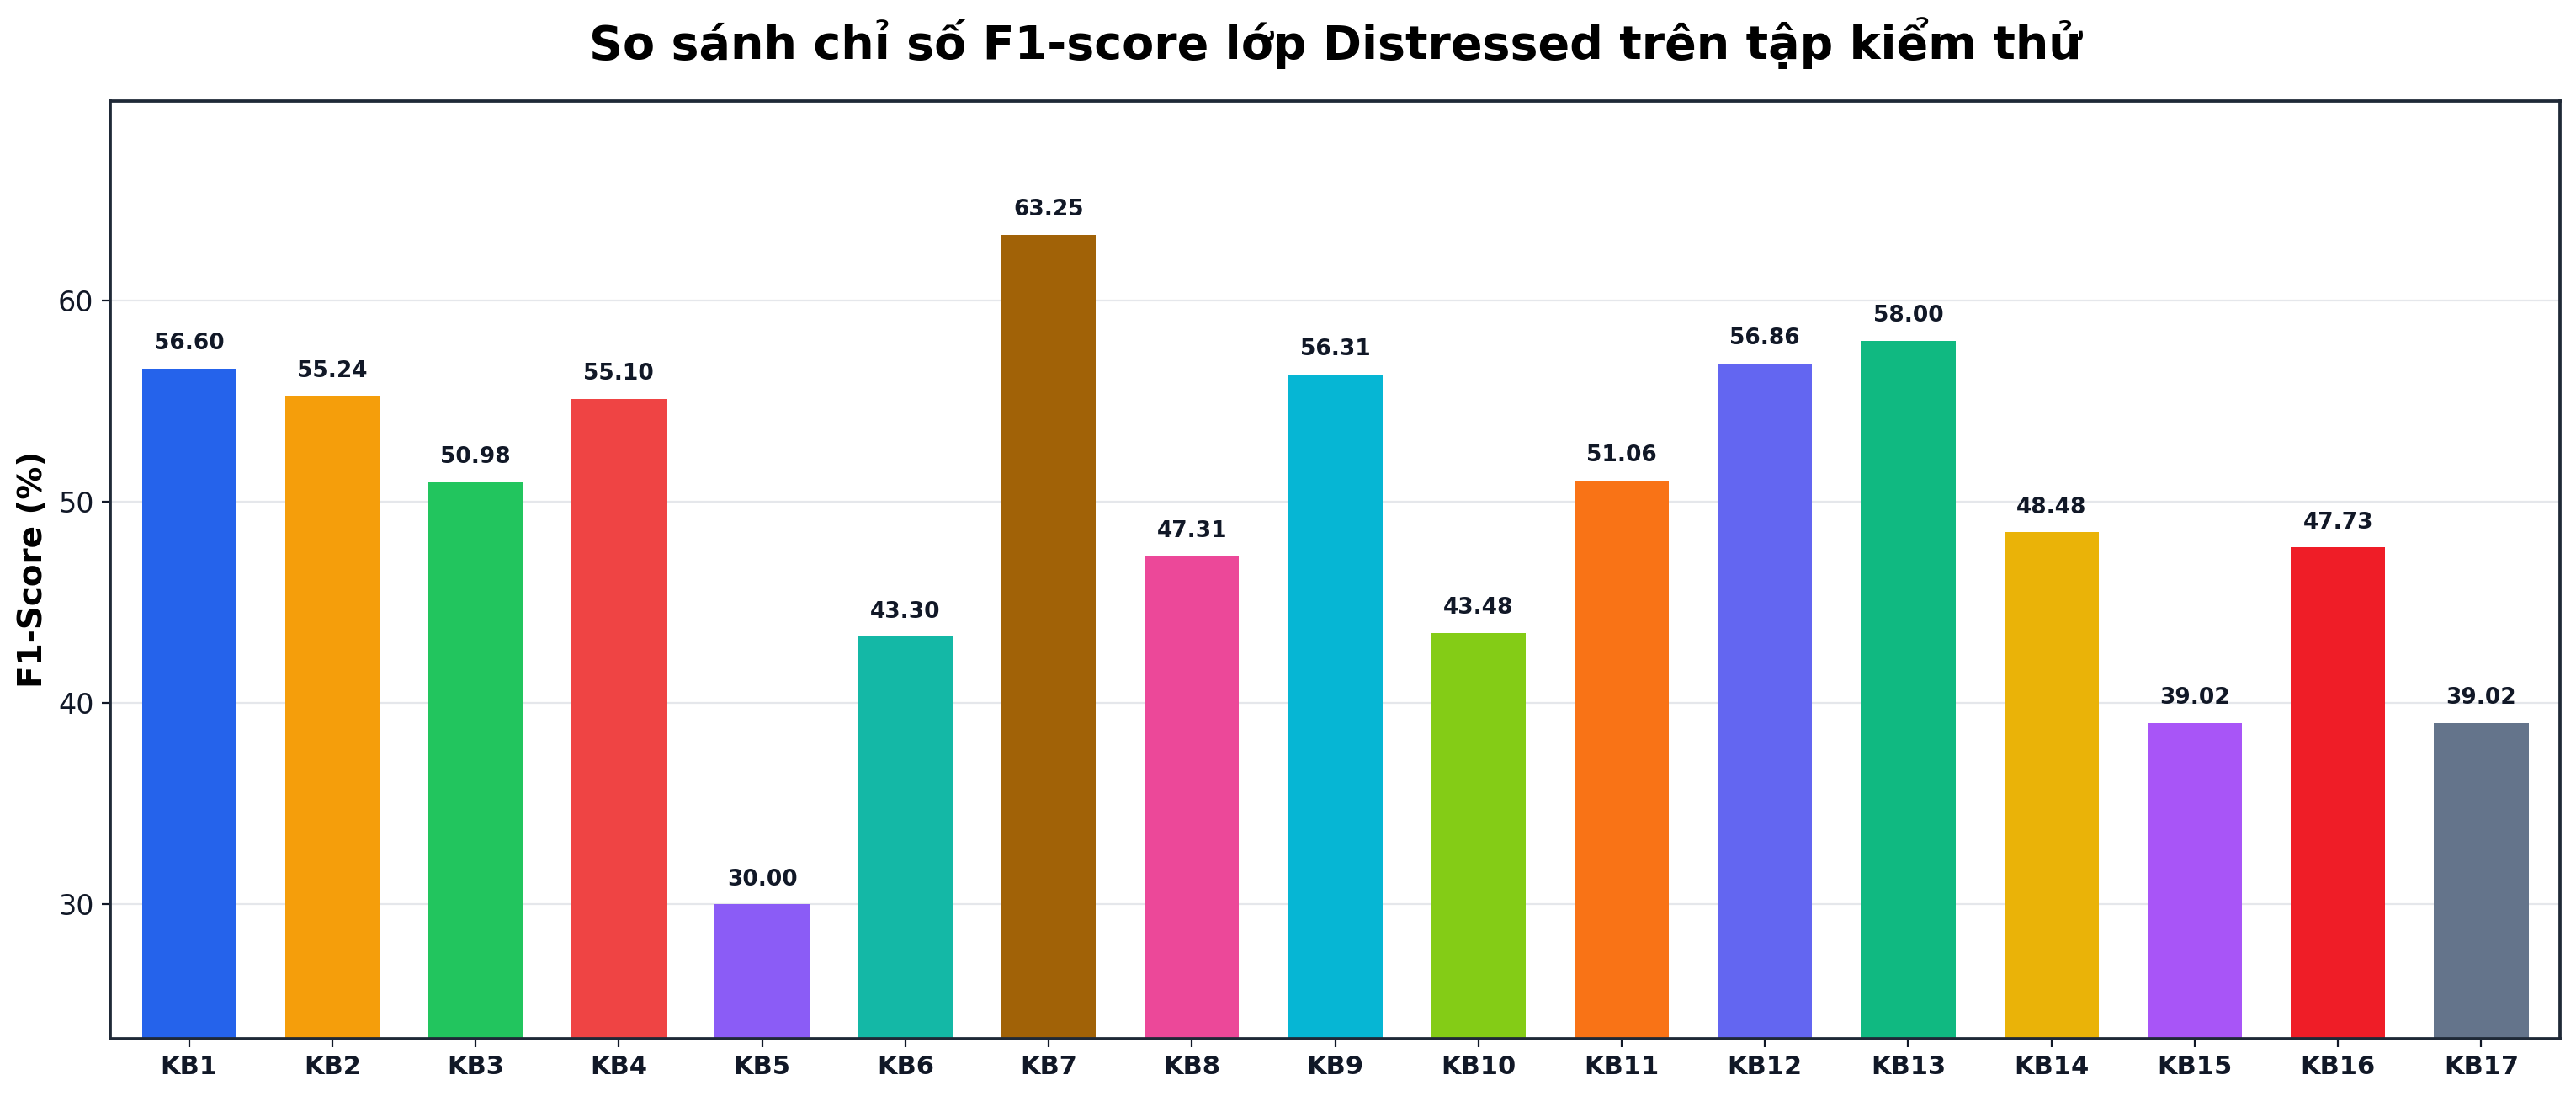
\includegraphics[width=\textwidth]{acc-loss/metric_f1_distressed_test.png}
    \caption{F1-score của lớp Distressed}
    \label{fig:F1-Score_distressed}
\end{subfigure}
\end{figure}

\begin{figure}[H]
\ContinuedFloat
\centering
\begin{subfigure}{\fairfigurewidth}
    \centering
    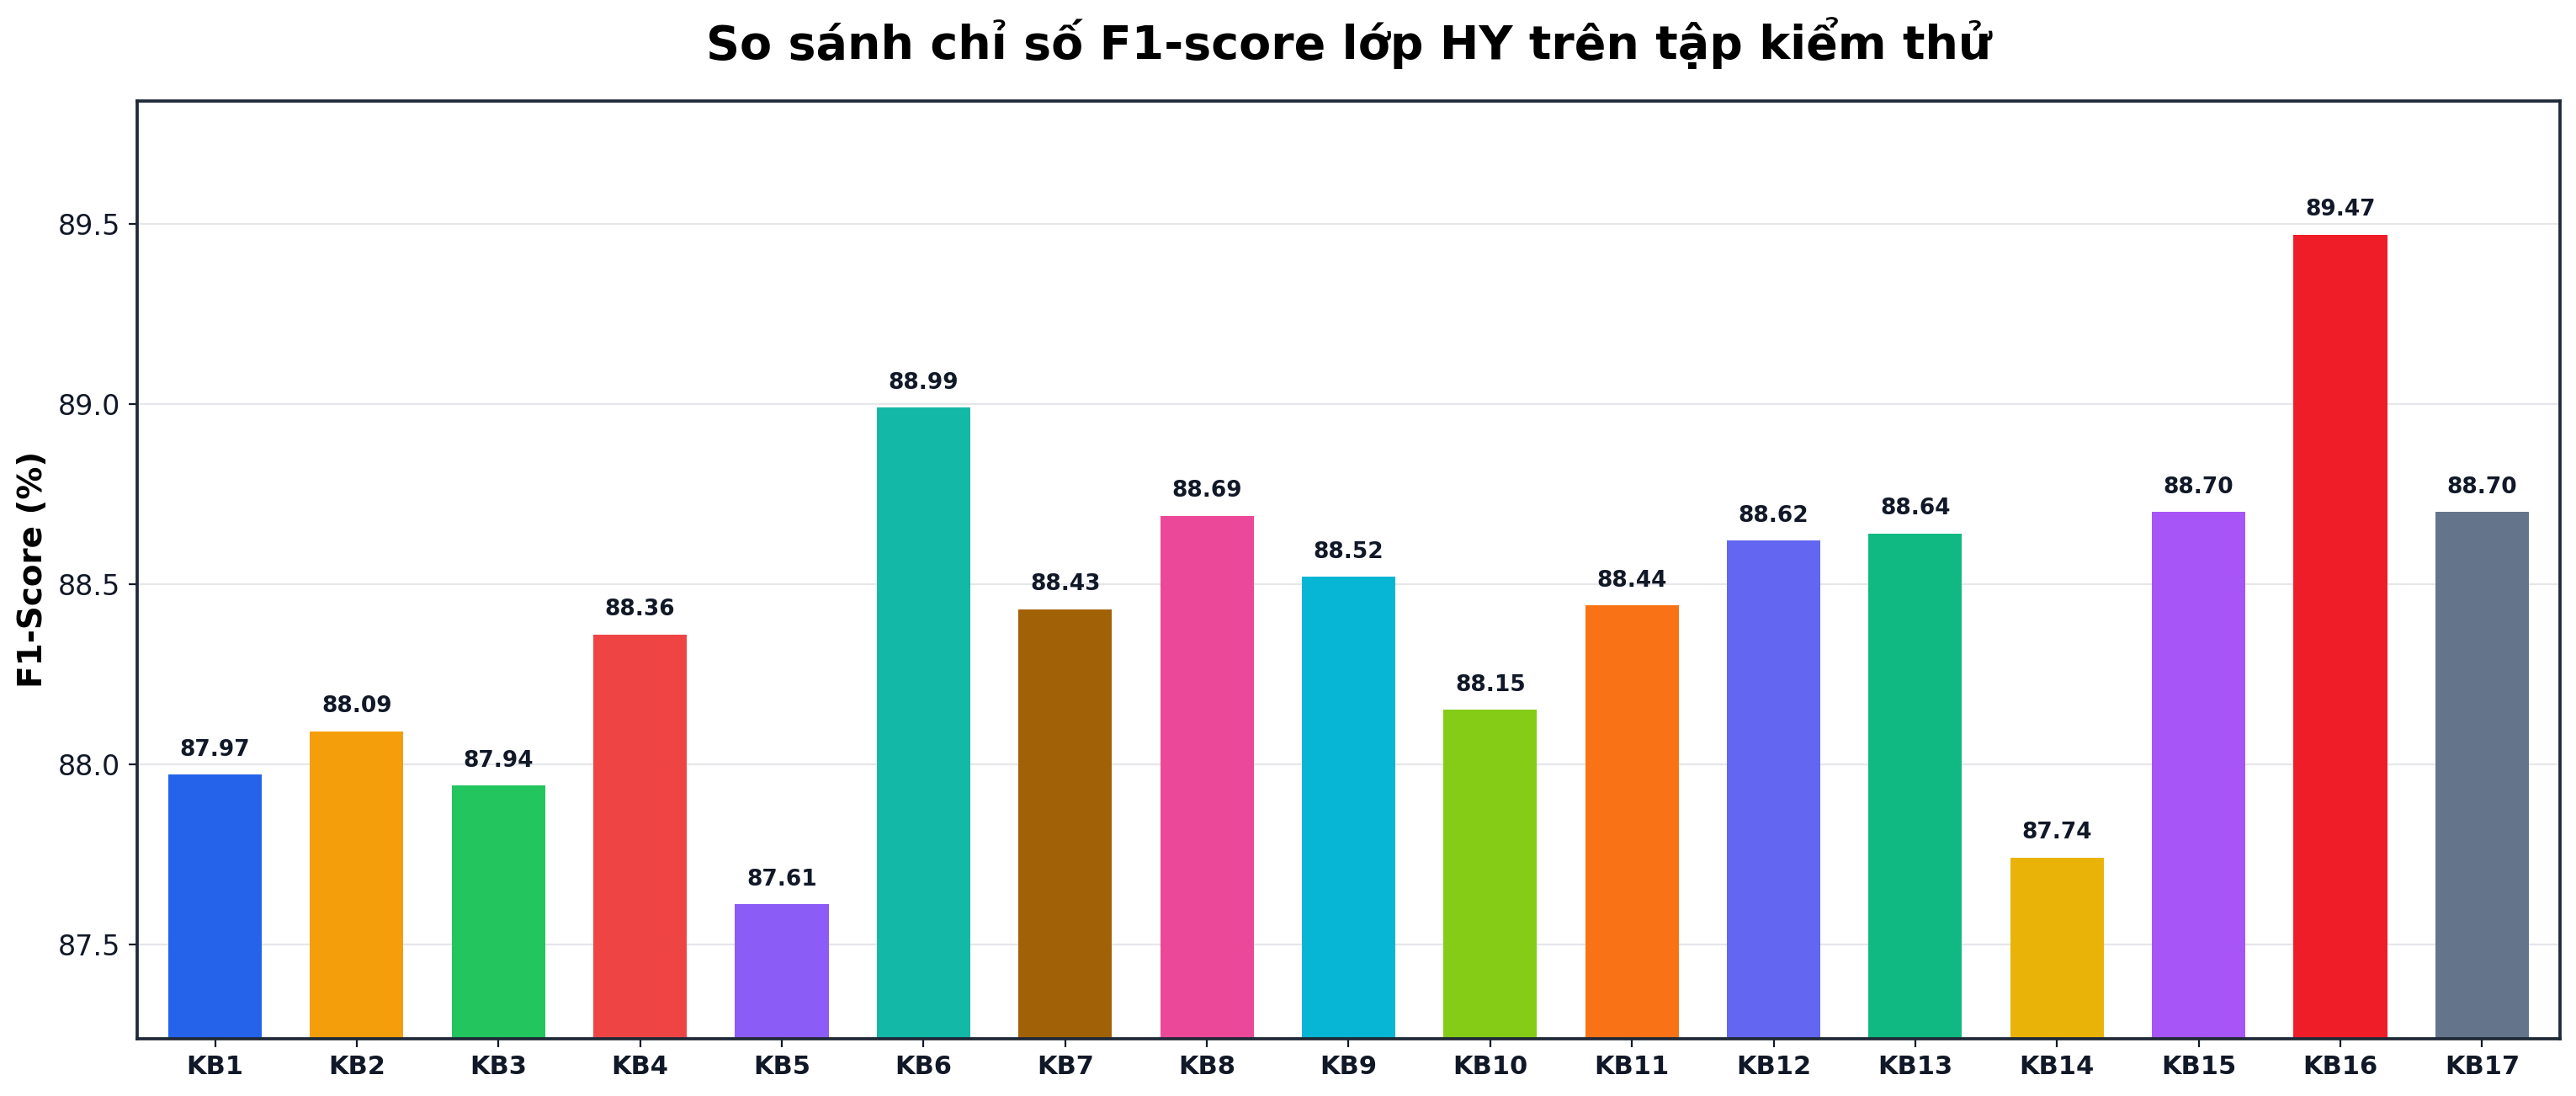
\includegraphics[width=\textwidth]{acc-loss/metric_f1_hy_test.png}
    \caption{F1-score của lớp HY (High Yield)}
    \label{fig:F1-Score_hy}
\end{subfigure}
\end{figure}

\begin{figure}[H]
\ContinuedFloat
\centering
\begin{subfigure}{\fairfigurewidth}
    \centering
    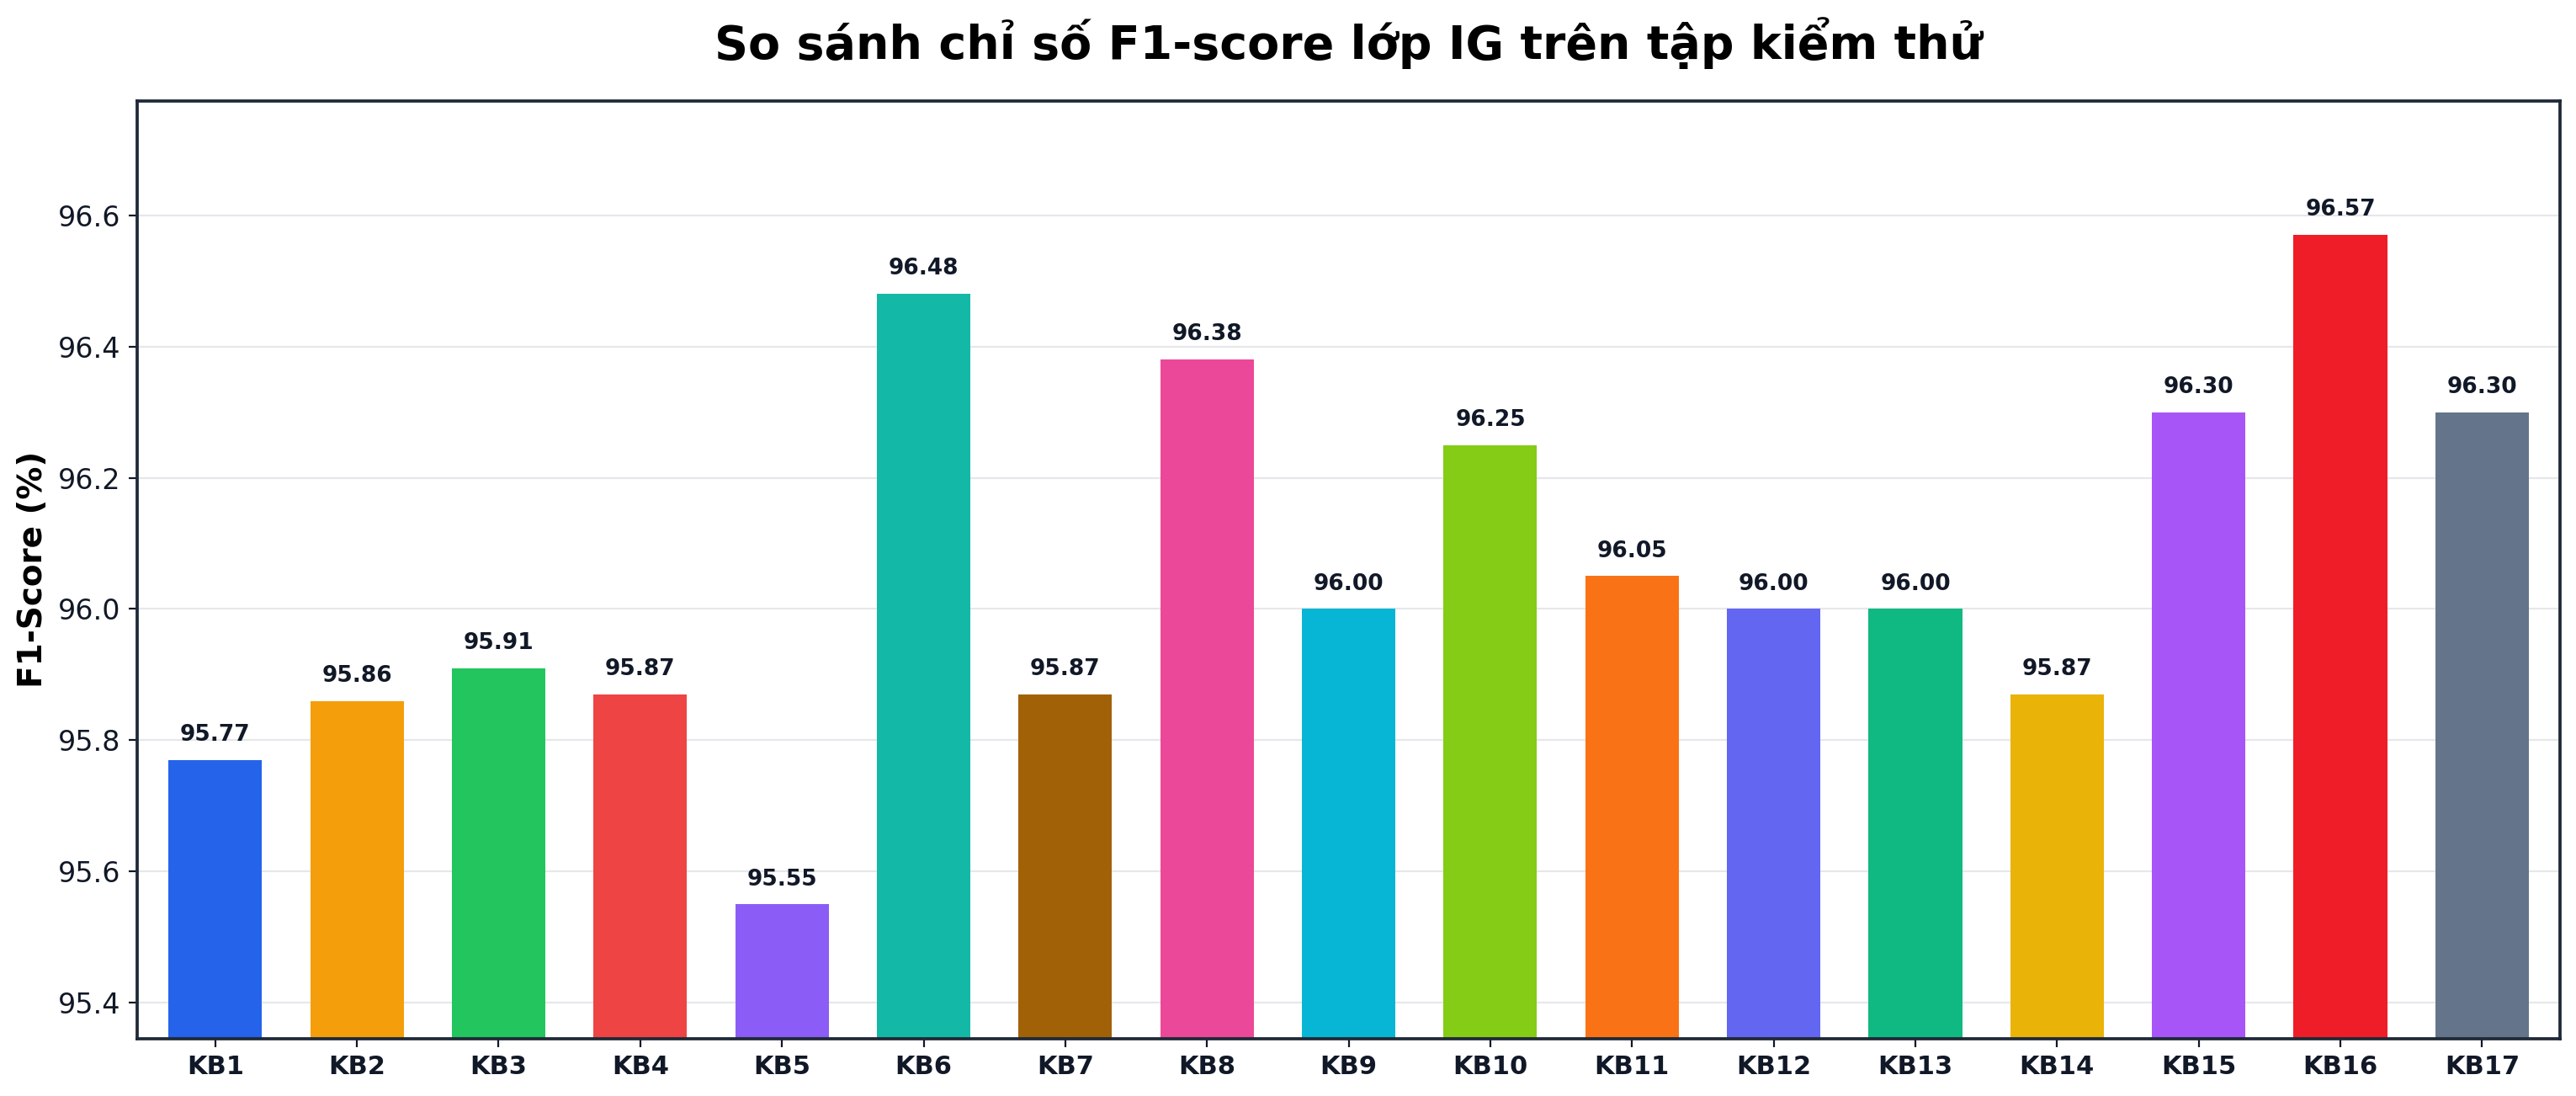
\includegraphics[width=\textwidth]{acc-loss/metric_f1_ig_test.png}
    \caption{F1-score của lớp IG (Investment Grade)}
    \label{fig:F1-Score_ig}
\end{subfigure}
\caption{F1-score lớp Distressed (a), lớp HY (b) và lớp IG (c) trên tập kiểm thử}
\label{fig:F1-Score_classes}
\end{figure}
F1-score phản ánh sự cân bằng giữa Precision và Recall của các mô hình trên từng lớp xếp hạng tín dụng. Kết quả cho thấy lớp Distressed có sự chênh lệch lớn nhất giữa các mô hình. GraphSAGE đạt F1-score cao nhất ở lớp Distressed với 63,25\%, cho thấy lợi thế trong nhận diện doanh nghiệp rủi ro cao. Các mô hình LightGBM, XGBoost và LSTM cũng đạt kết quả tương đối tốt, trong khi PatchTST có F1-score thấp nhất ở lớp này. Ở nhóm Fuzzy Ensemble, FR-TTLPXL đạt kết quả tốt nhất cho lớp Distressed với 58,00\%.Các kịch bản DMF chưa thật sự nổi bật ở lớp Distressed, cho thấy việc phát hiện nhóm rủi ro cao vẫn còn khó khăn. Đối với lớp HY, F1-score của các mô hình khá ổn định, chủ yếu quanh mức 88\%–89\%.DMF-TG đạt F1-score cao nhất ở lớp HY với 89,47\%.
Ở lớp IG, hầu hết các mô hình đều đạt F1-score cao, trong đó DMF-TG tiếp tục dẫn đầu với 96,57\%.Nhìn chung, GraphSAGE phù hợp hơn khi ưu tiên lớp Distressed, còn DMF-TG nổi bật ở hai lớp HY và IG.



\subsubsection{AUC-ROC của các kịch bản}

\begin{figure}[H]
\centering
\setupfairsubfigures
\begin{subfigure}{\fairfigurewidth}
    \centering
    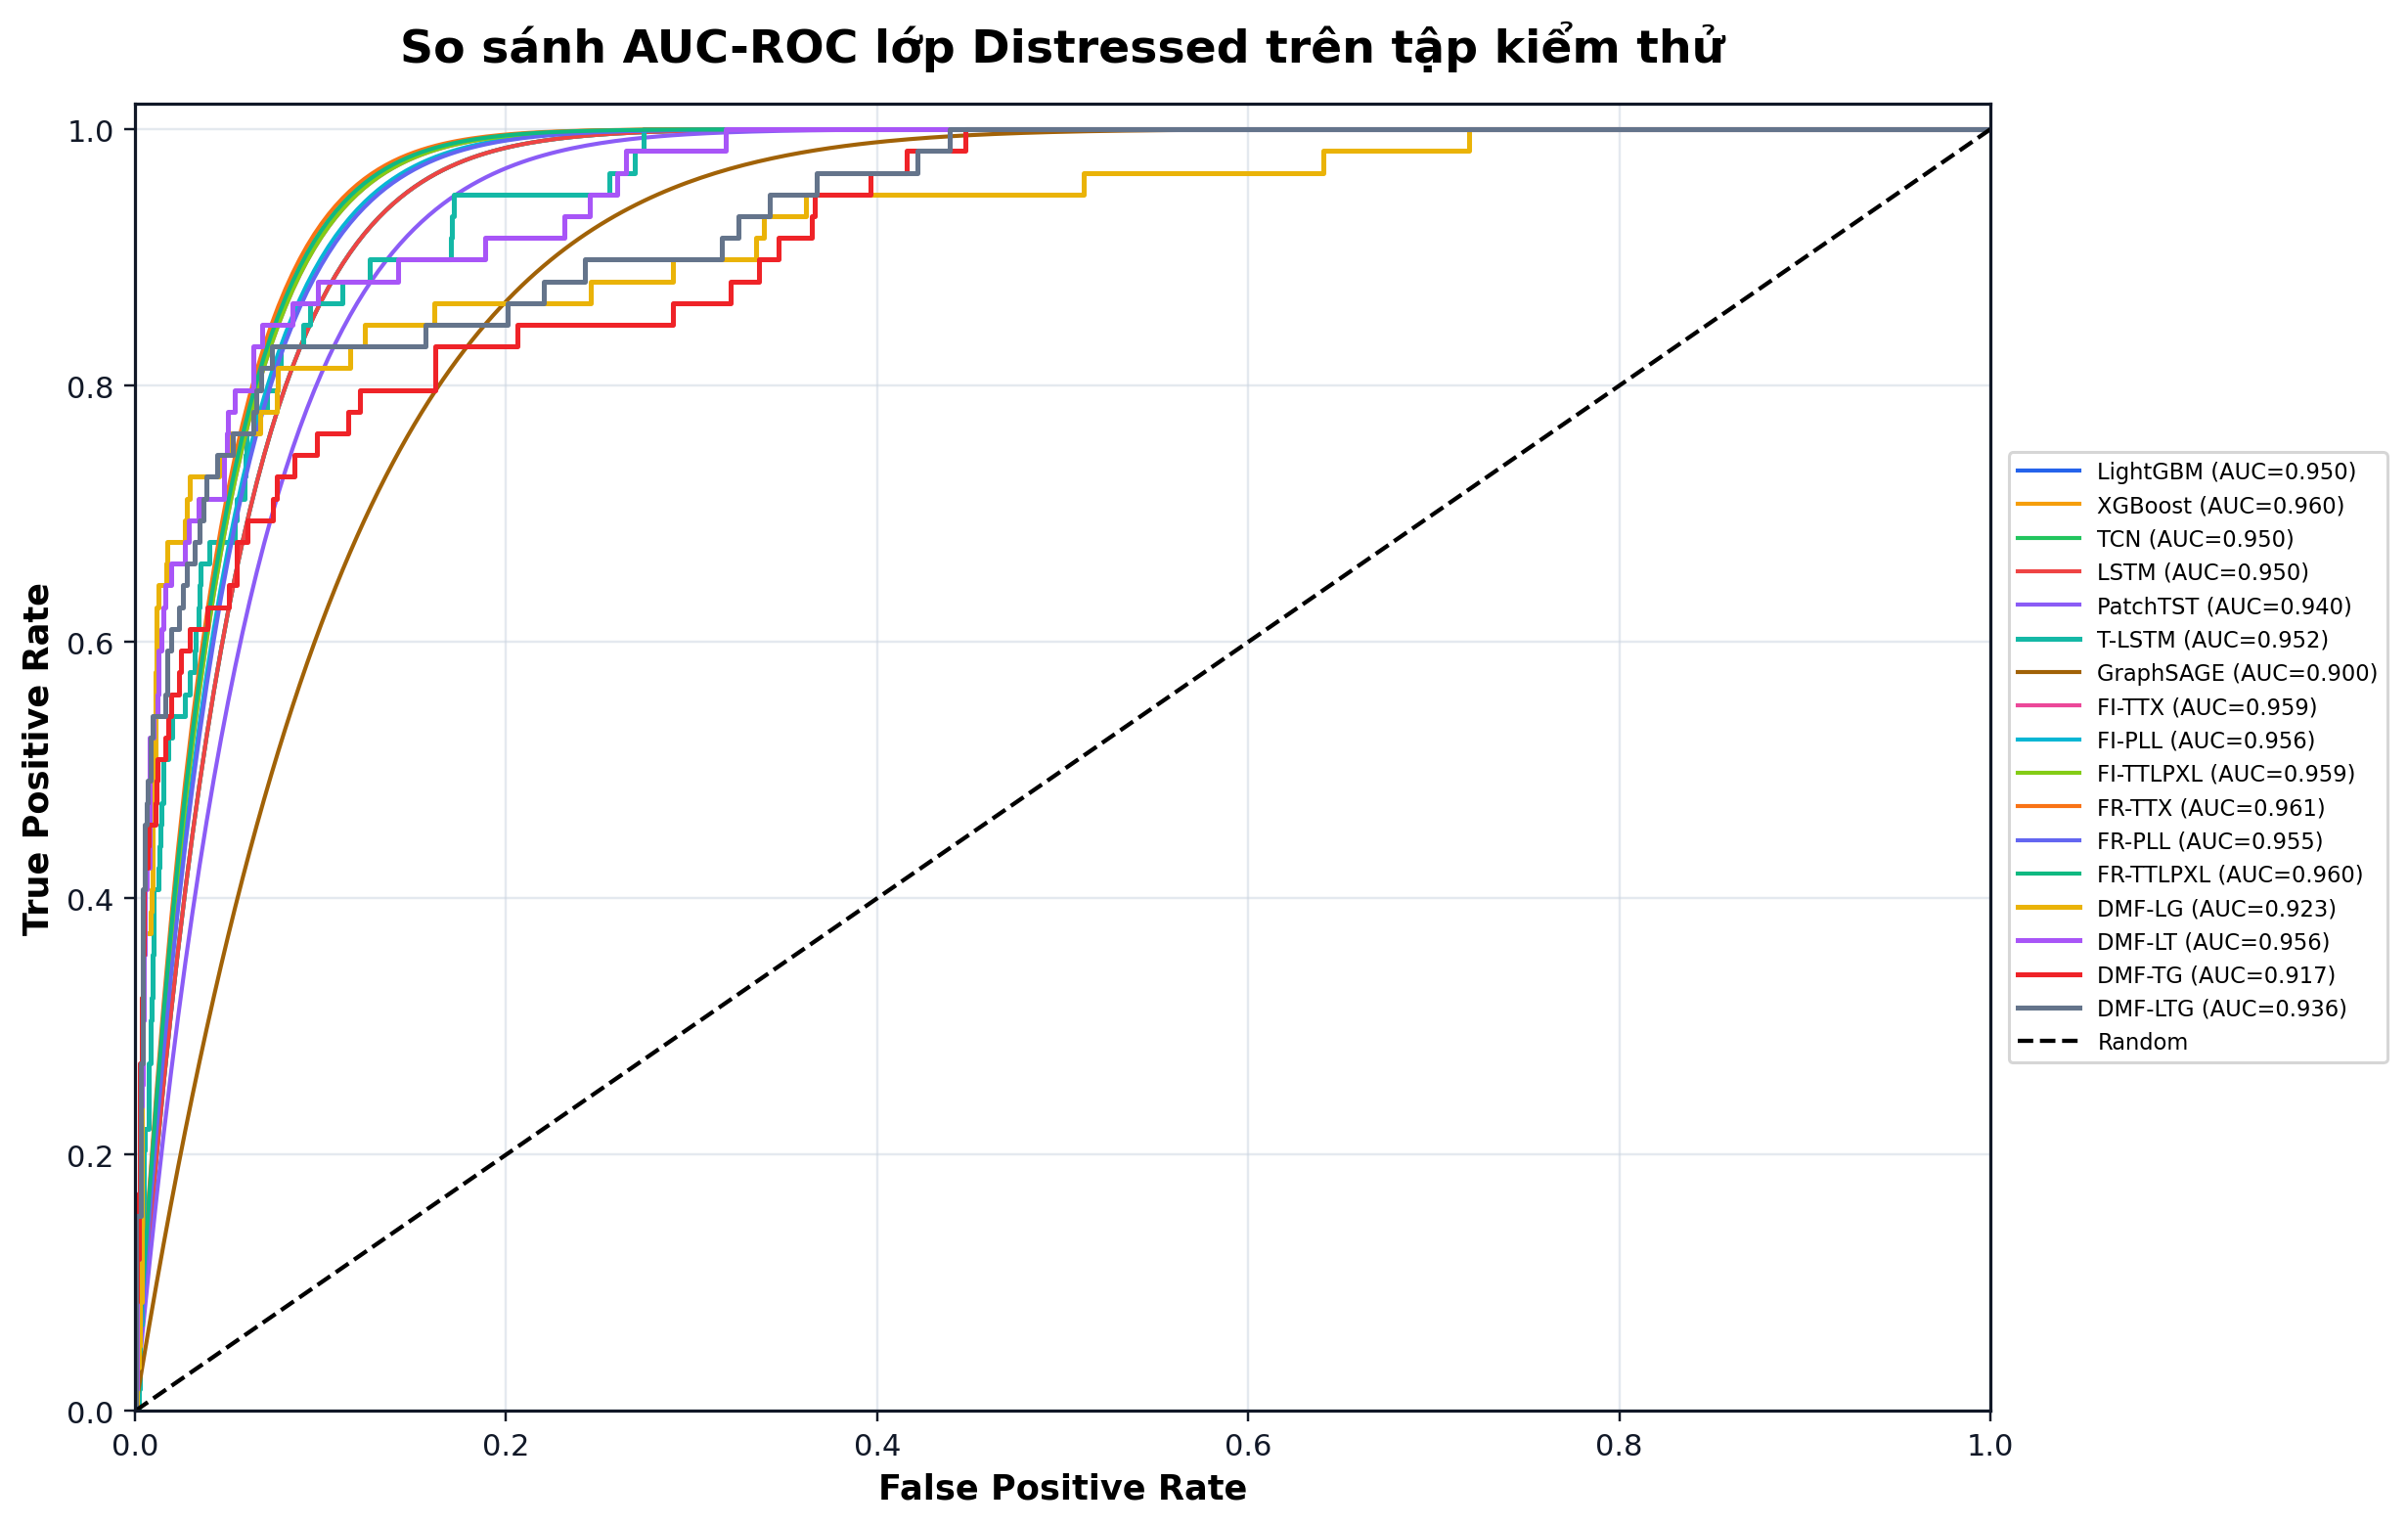
\includegraphics[width=\textwidth]{acc-loss/roc_distressed_17_models.png}
    \caption{Đường cong ROC trên lớp Distressed}
    \label{fig:AUC-ROC_distressed}
\end{subfigure}
\end{figure}

\begin{figure}[H]
\ContinuedFloat
\centering
\begin{subfigure}{\fairfigurewidth}
    \centering
    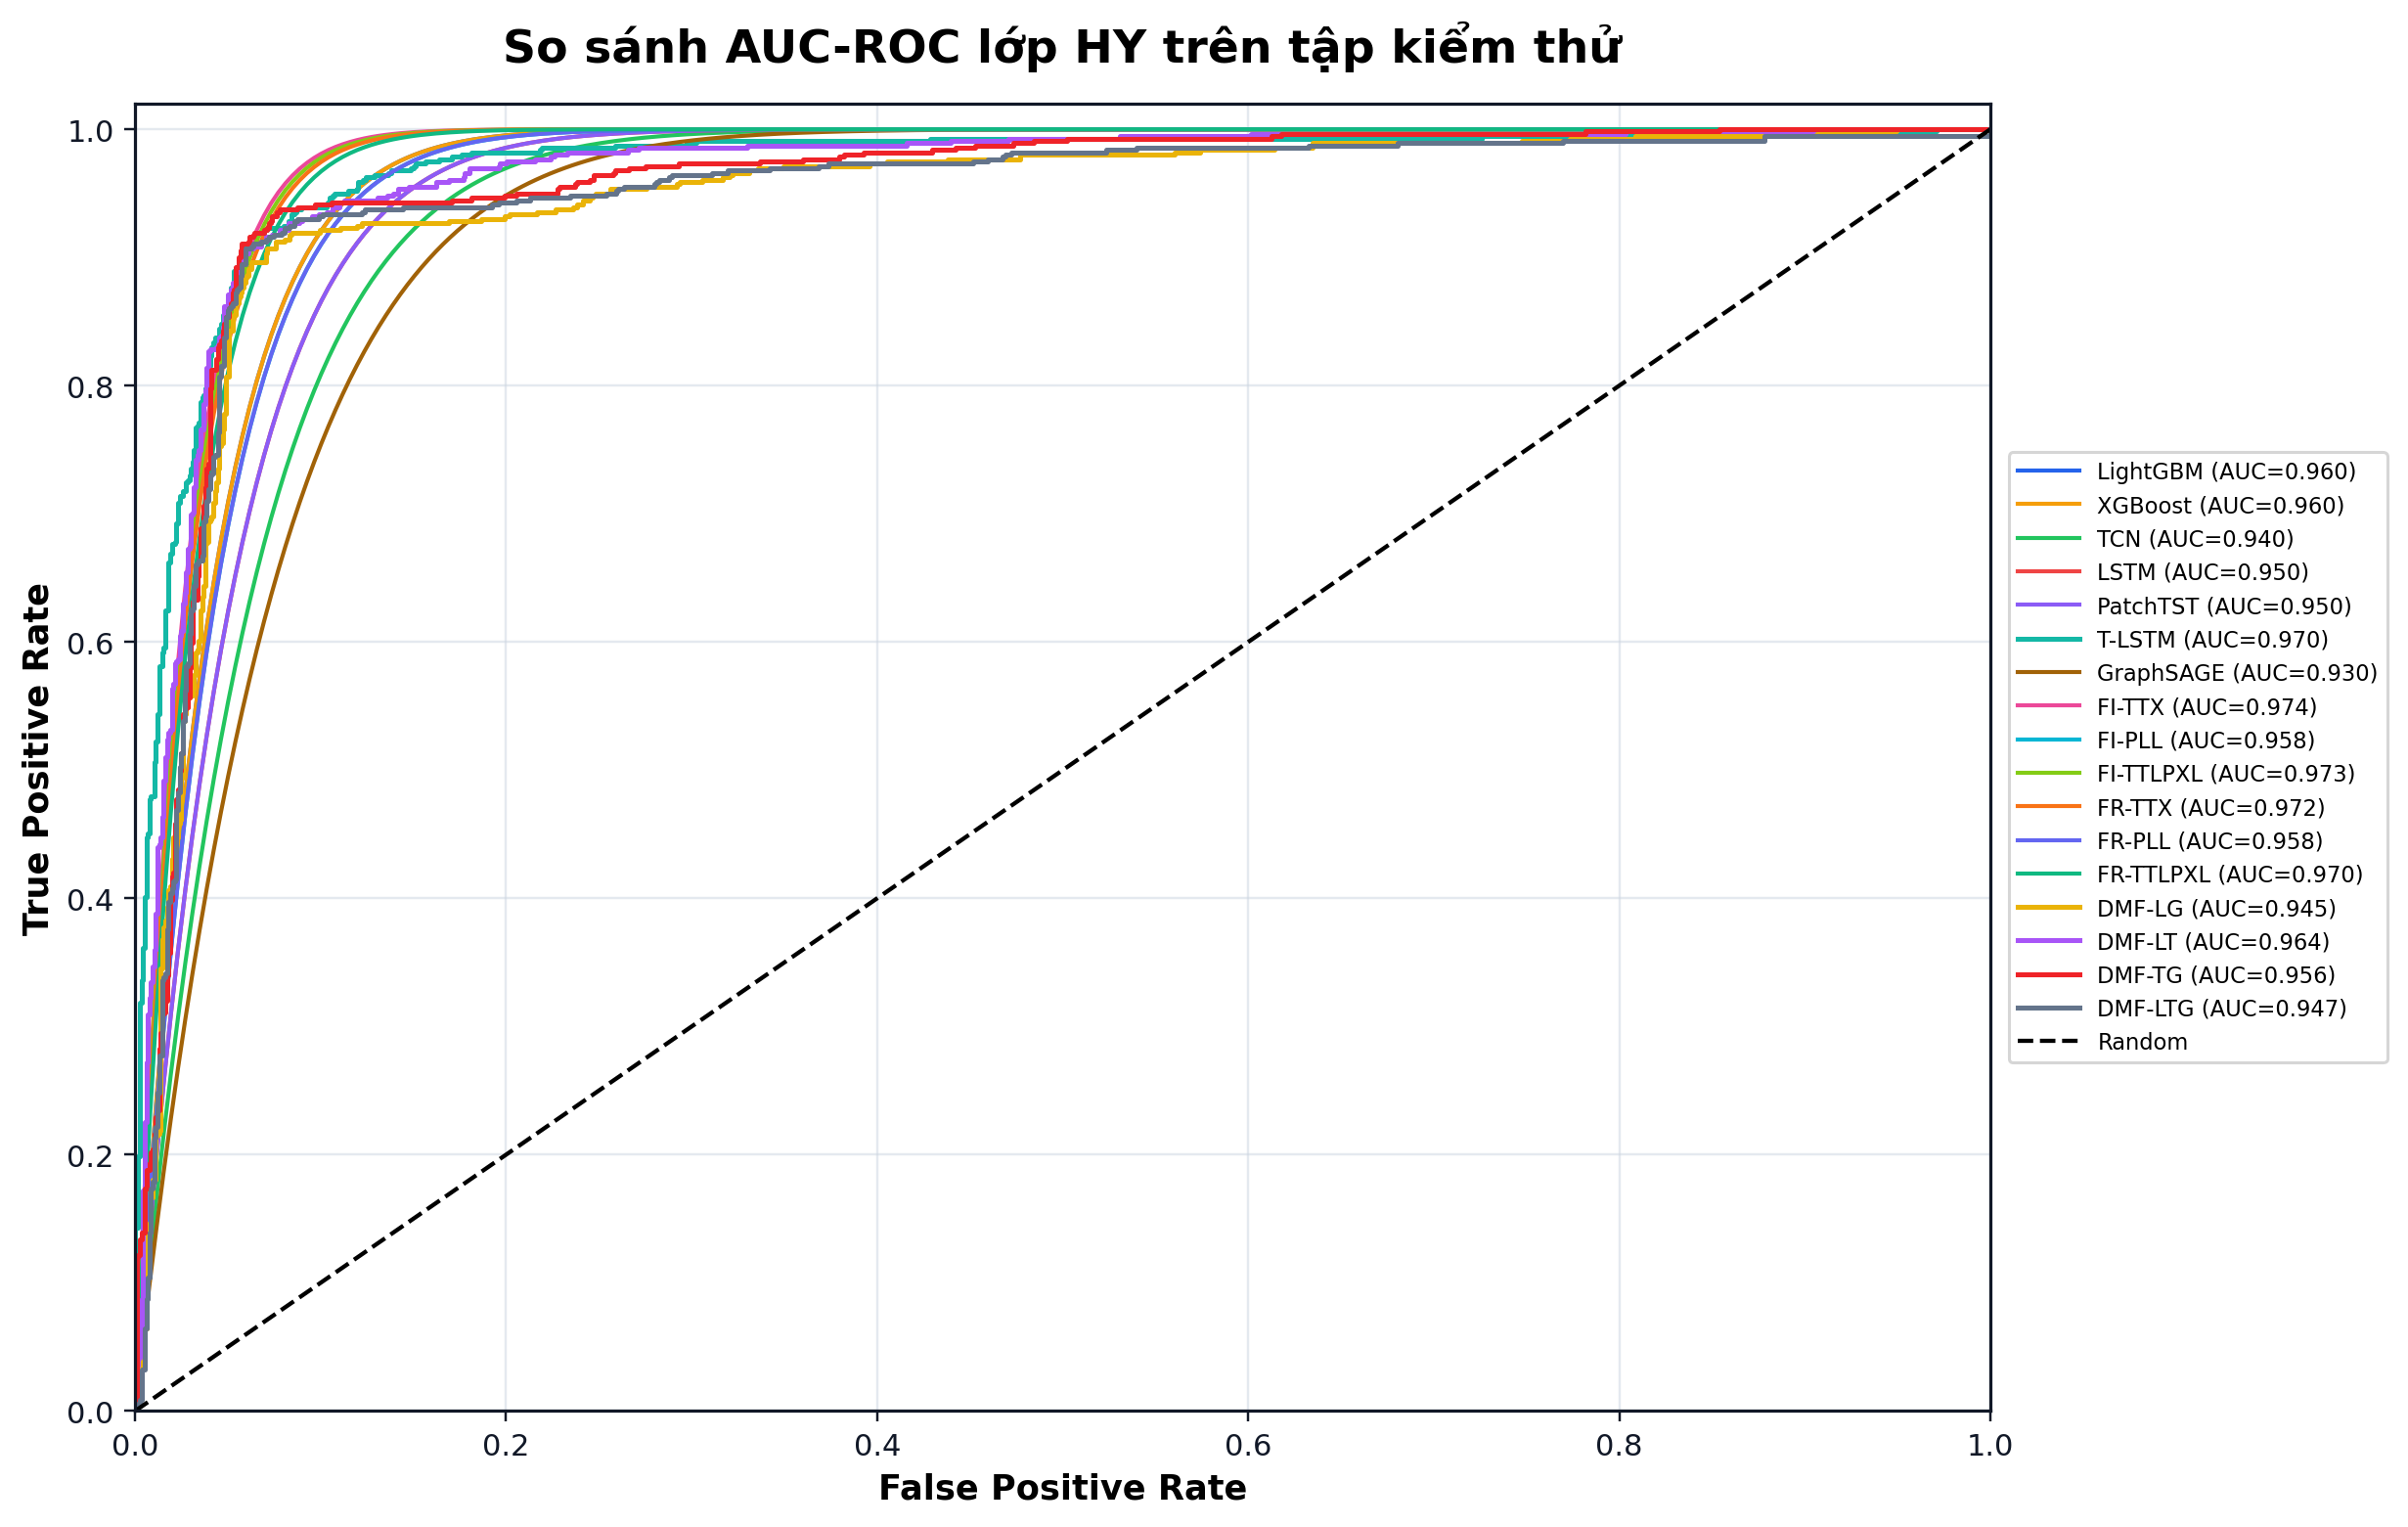
\includegraphics[width=\textwidth]{acc-loss/roc_hy_17_models.png}
    \caption{Đường cong ROC trên lớp HY (High Yield)}
    \label{fig:AUC-ROC_hy}
\end{subfigure}
\end{figure}

\begin{figure}[H]
\ContinuedFloat
\centering
\begin{subfigure}{\fairfigurewidth}
    \centering
    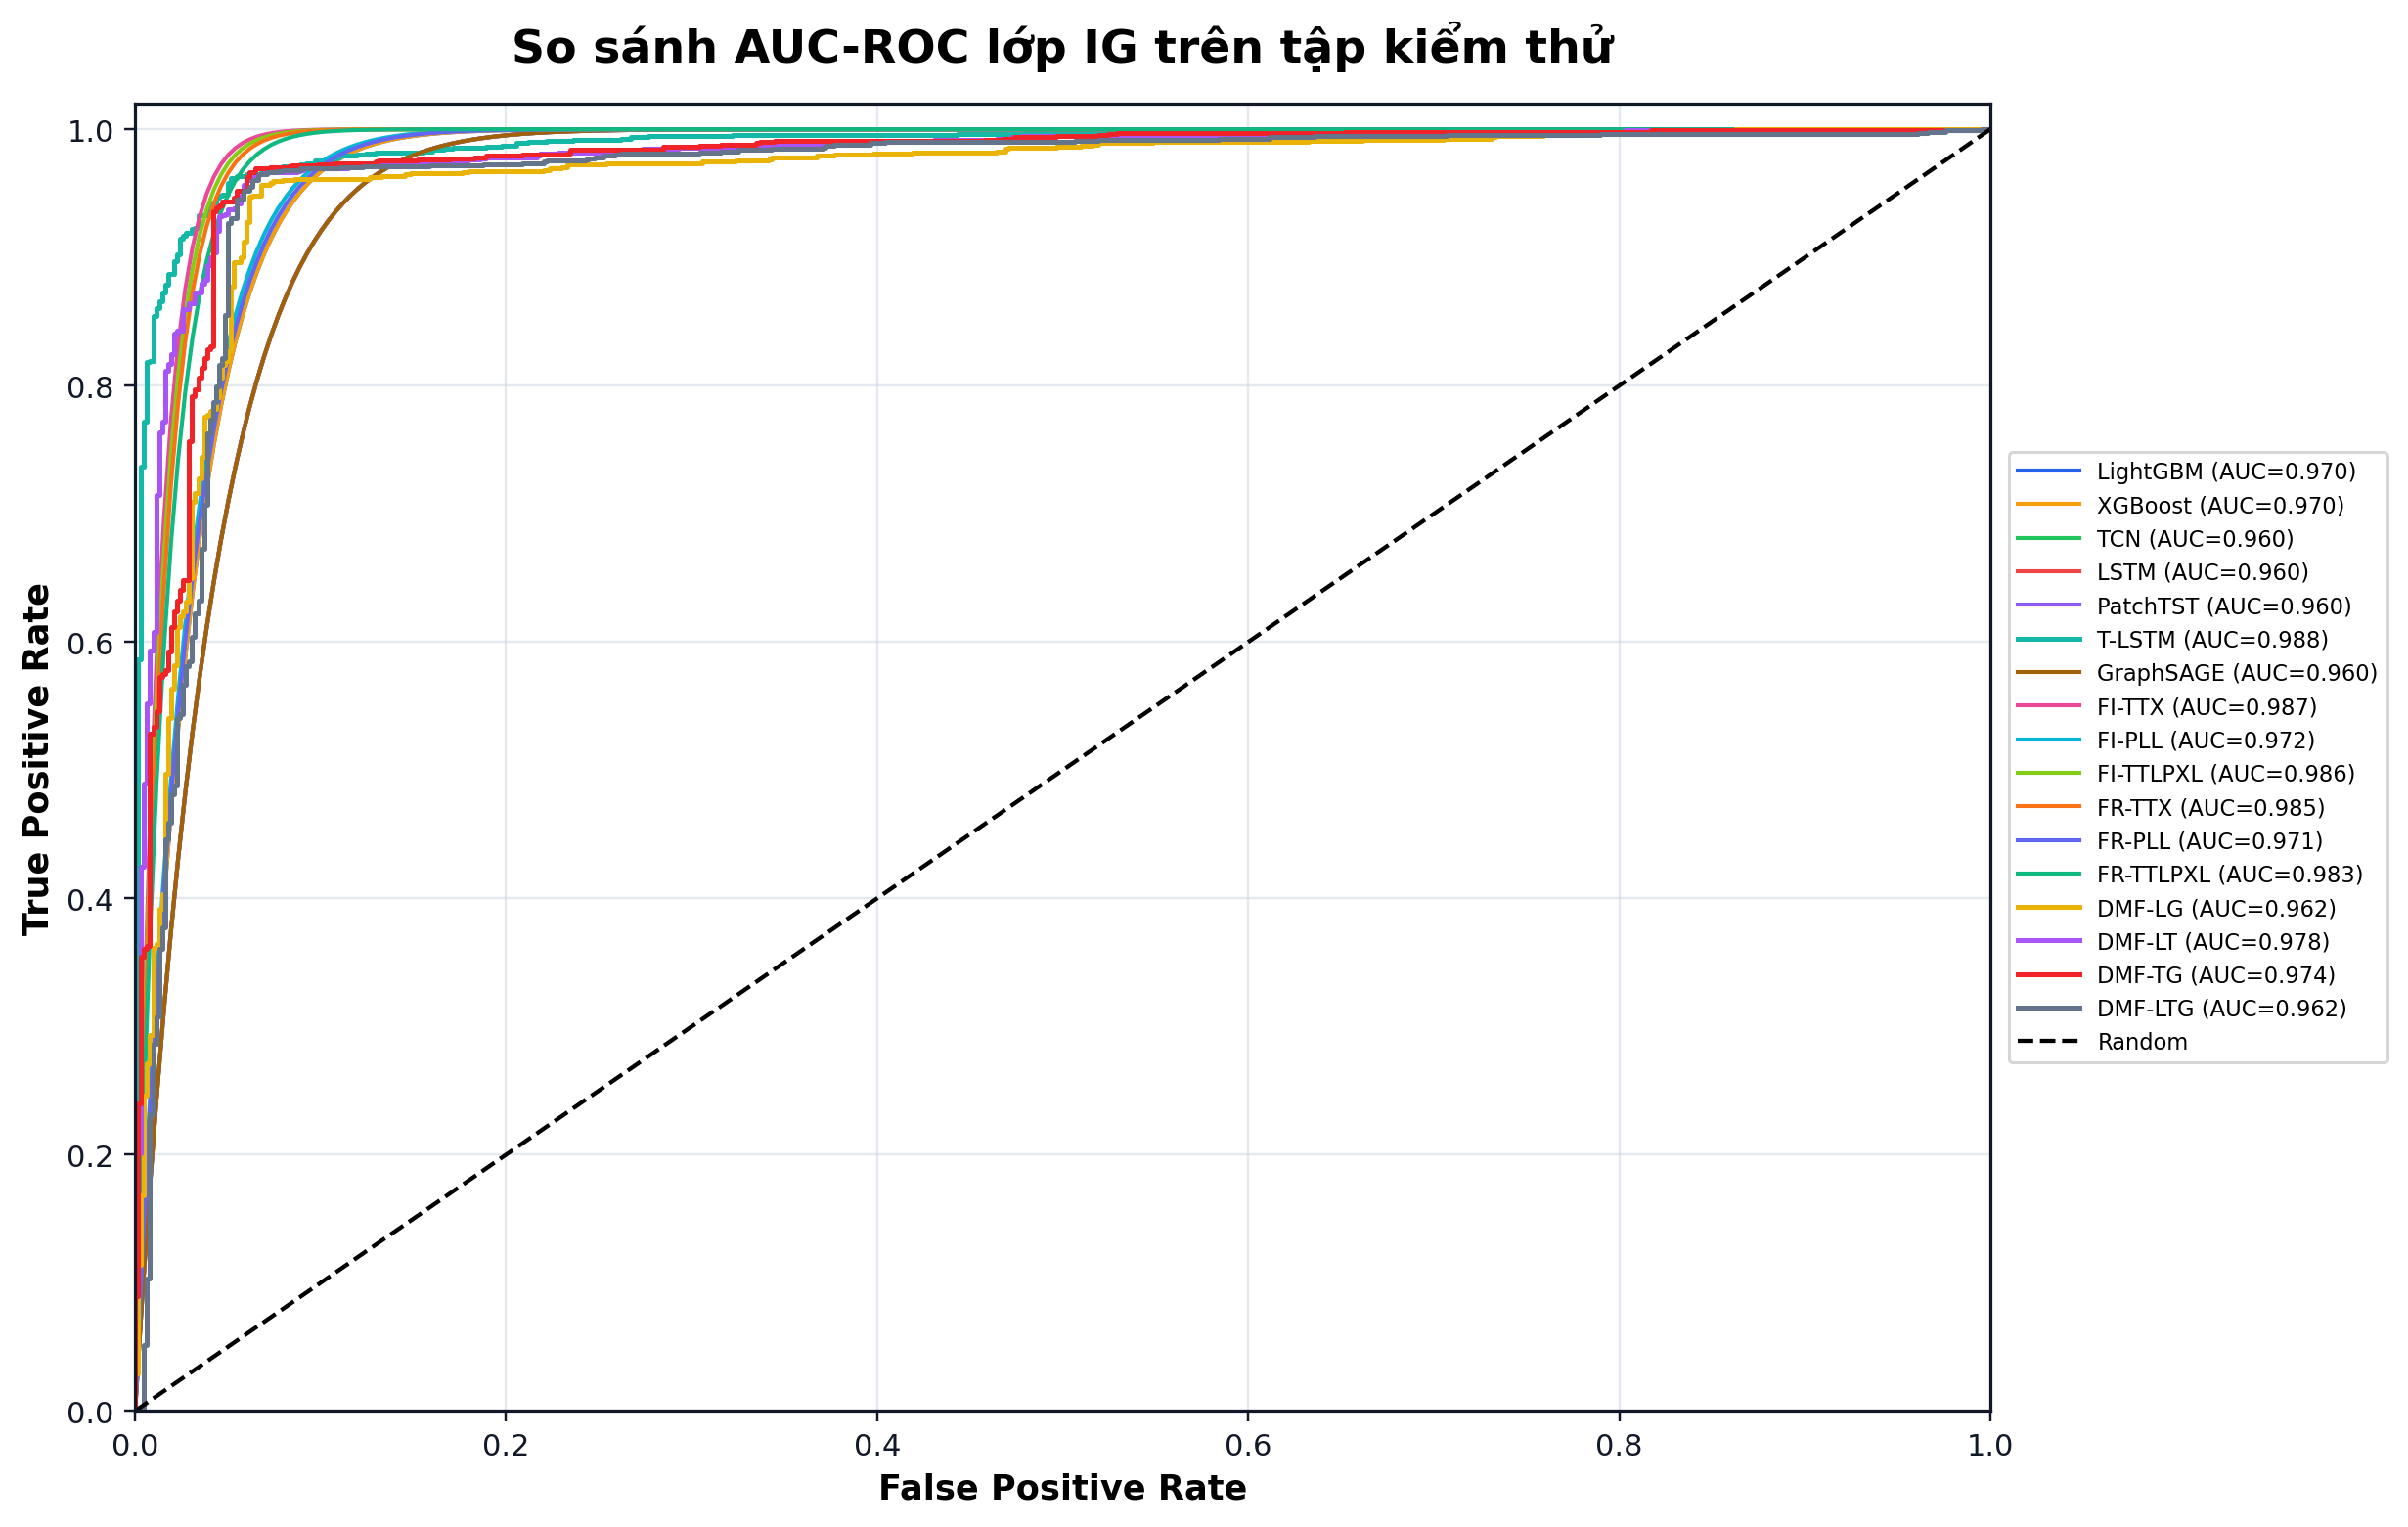
\includegraphics[width=\textwidth]{acc-loss/roc_ig_17_models.png}
    \caption{Đường cong ROC trên lớp IG (Investment Grade)}
    \label{fig:AUC-ROC_ig}
\end{subfigure}
\caption{AUC-ROC lớp Distressed (a), lớp HY (b) và lớp IG (c) trên tập kiểm thử}
\label{fig:AUC-ROC_classes}
\end{figure}

Ba biểu đồ ROC cho thấy hầu hết các mô hình đều có đường cong nằm xa đường chéo ngẫu nhiên, chứng tỏ khả năng phân biệt tốt giữa từng lớp xếp hạng và các lớp còn lại. Ở lớp Distressed, FR-TTX đạt AUC cao nhất với 96.1\%, tiếp theo là XGBoost và FR-TTLPXL cùng đạt 96\%. Đối với lớp HY, FI-TTX đạt kết quả tốt nhất với AUC 97.4\%, cho thấy hiệu quả của Fuzzy Ensemble trong phân biệt nhóm rủi ro trung bình. Ở lớp IG, T-LSTM đạt AUC cao nhất với 98.8\%, phản ánh khả năng nhận diện rất tốt nhóm doanh nghiệp có chất lượng tín dụng cao. Nhìn chung, các kịch bản Fuzzy Ensemble như FI-TTX, FR-TTX và FI-TTLPXL đạt AUC nổi bật ở nhiều lớp, trong khi DMF có độ chính xác tổng thể cao nhưng chưa phải mô hình có AUC tốt nhất theo từng lớp.

\subsubsection{Thời gian kiểm thử}
\begin{figure}[H]
    \centering % Căn giữa hình ảnh
    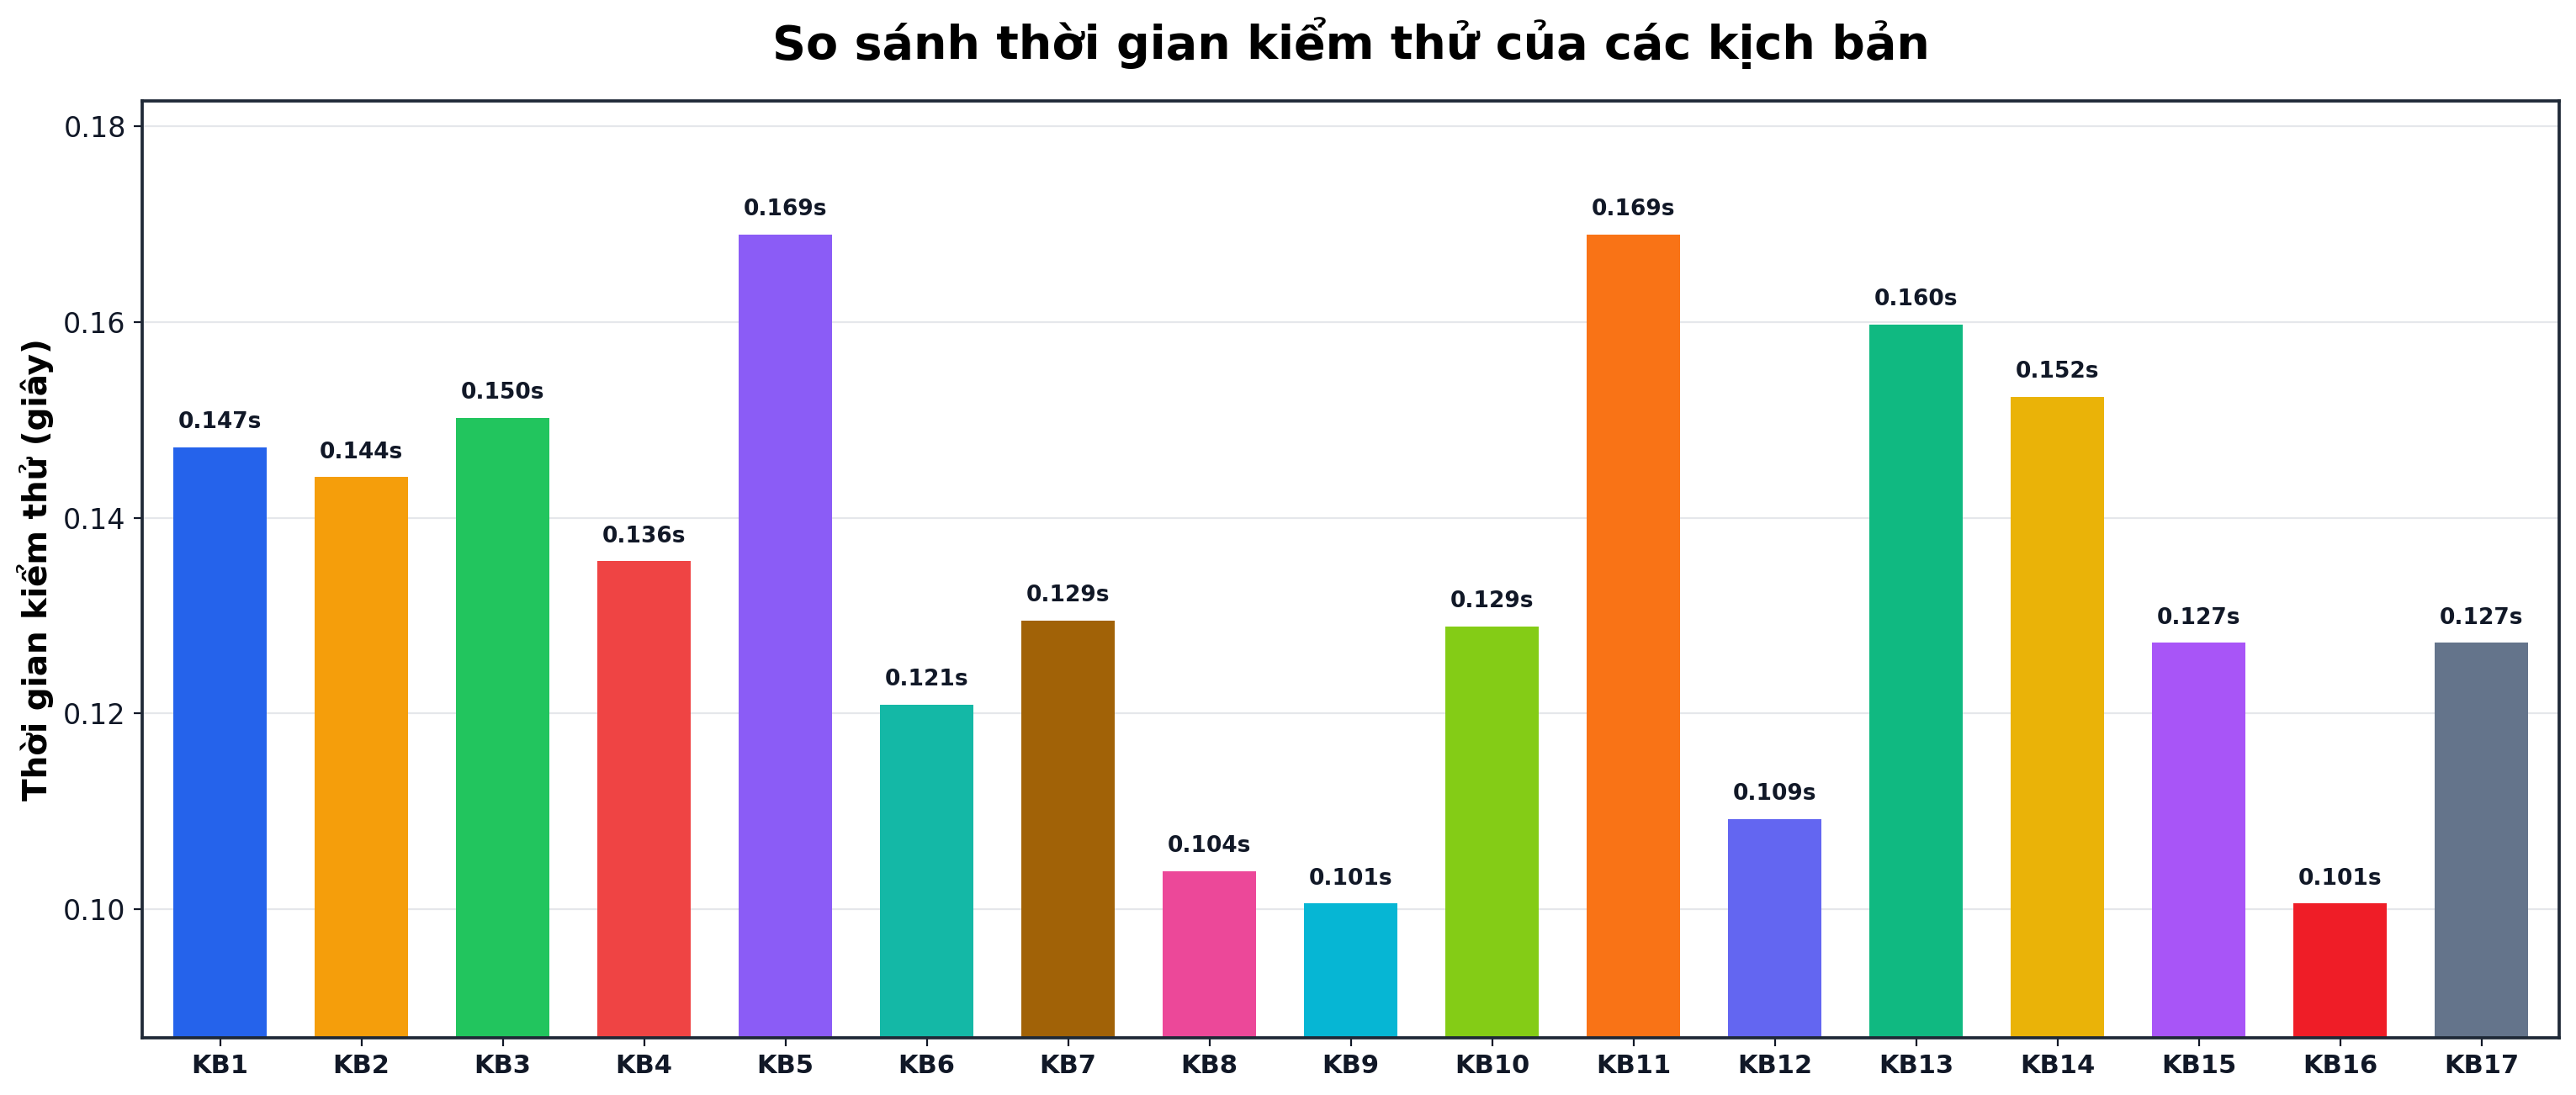
\includegraphics[width=\fairfigurewidth]{acc-loss/metric_inference_time_test_scenarios.png} % Thay 'ten-file-anh' bằng tên ảnh của bạn (không cần đuôi .png/.jpg)
    \caption{Thời gian kiểm thử của các kịch bản} % Dòng chú thích dưới ảnh
\end{figure}
Kết quả kiểm thử cho thấy thời gian suy luận của 17 mô hình và kịch bản kết hợp đều ở mức rất thấp, dao động từ 0,101 giây đến 0,169 giây. Điều này chứng minh các mô hình có khả năng dự đoán nhanh và phù hợp với yêu cầu triển khai thực tế. Trong nhóm mô hình đơn lẻ, T-LSTM đạt thời gian kiểm thử thấp nhất với 0,121 giây, trong khi PatchTST có thời gian cao nhất với 0,169 giây. Các mô hình còn lại như GraphSAGE, LSTM, LightGBM, XGBoost và TCN có thời gian kiểm thử tương đối ổn định. Đối với nhóm Fuzzy Ensemble, FI-PLL và FI-TTX cho tốc độ suy luận nhanh, lần lượt đạt 0,101 giây và 0,104 giây. Trong nhóm Dynamic Model Fusion, DMF-TG đạt thời gian kiểm thử thấp nhất với 0,101 giây. 
\subsubsection{Kết quả giải thích bằng XAI}
\paragraph{GradientSHAP}
GradientSHAP được sử dụng để đo lường mức độ đóng góp của từng chỉ số tài chính vào xác suất dự báo của mô hình. Phương pháp này được triển khai trực tiếp trên mô hình đã huấn luyện, không sử dụng mô hình thay thế. Các đặc trưng chuỗi tài chính được rút gọn bằng giá trị trung bình theo cửa sổ thời gian, sau đó GradientSHAP ước lượng mức đóng góp của từng biến thông qua nhiều lần lấy mẫu giữa mẫu cần giải thích và tập nền.

\xairesultfigure{Kết quả GradientSHAP của kịch bản 1}{gradientshap-scenario-1}{acc-loss/xai_shap_lightgbm.png}

Hình 4.10 trình bày kết quả giải thích mô hình LightGBM bằng phương pháp GradientSHAP. Trục hoành thể hiện giá trị trung bình tuyệt đối của mức đóng góp \(\mathrm{mean}\left(\left|\mathrm{GradientSHAP\ attribution}\right|\right)\), còn trục tung là các chỉ số tài chính đầu vào. Thanh càng dài cho thấy đặc trưng đó có ảnh hưởng càng lớn đến xác suất dự báo của mô hình.
Kết quả cho thấy Pretax Profit Margin, Operating Profit Margin, Debt Equity Ratio và Current Ratio là các đặc trưng có mức ảnh hưởng cao nhất. Điều này cho thấy mô hình LightGBM chủ yếu dựa vào khả năng sinh lời, mức độ đòn bẩy và khả năng thanh khoản để đưa ra quyết định xếp hạng tín dụng. Các chỉ số như Ebit Margin, Operating Cashflow PS và Net Profit Margin cũng có đóng góp đáng kể, phản ánh vai trò của lợi nhuận và dòng tiền trong đánh giá sức khỏe tài chính doanh nghiệp. Ngược lại, các đặc trưng như Asset Turnover, Gross Profit Margin và ROE có mức ảnh hưởng thấp hơn trong kịch bản này.
Đây cũng là cơ sở để so sánh tương tự với các kịch bản còn lại, nhằm xác định xem các mô hình khác có cùng tập trung vào các nhóm chỉ số tài chính quan trọng hay không.


\xairesultfigure{Kết quả GradientSHAP của kịch bản 2}{gradientshap-scenario-2}{acc-loss/xai_shap_xgboost.png}

\xairesultfigure{Kết quả GradientSHAP của kịch bản 3}{gradientshap-scenario-3}{acc-loss/xai_shap_tcn.png}

\xairesultfigure{Kết quả GradientSHAP của kịch bản 4}{gradientshap-scenario-4}{acc-loss/xai_shap_lstm.png}

\xairesultfigure{Kết quả GradientSHAP của kịch bản 5}{gradientshap-scenario-5}{acc-loss/xai_shap_patchtst.png}

\xairesultfigure{Kết quả GradientSHAP của kịch bản 6}{gradientshap-scenario-6}{acc-loss/xai_shap_tlstm.png}

\xairesultfigure{Kết quả GradientSHAP của kịch bản 7}{gradientshap-scenario-7}{acc-loss/xai_shap_graphsage.png}

\xairesultfigure{Kết quả GradientSHAP của kịch bản 8}{gradientshap-scenario-8}{acc-loss/xai_shap_fi_ttx.png}

\xairesultfigure{Kết quả GradientSHAP của kịch bản 9}{gradientshap-scenario-9}{acc-loss/xai_shap_fi_pll.png}

\xairesultfigure{Kết quả GradientSHAP của kịch bản 10}{gradientshap-scenario-10}{acc-loss/xai_shap_fi_ttlpxl.png}

\xairesultfigure{Kết quả GradientSHAP của kịch bản 11}{gradientshap-scenario-11}{acc-loss/xai_shap_fr_ttx.png}

\xairesultfigure{Kết quả GradientSHAP của kịch bản 12}{gradientshap-scenario-12}{acc-loss/xai_shap_fr_pll.png}

\xairesultfigure{Kết quả GradientSHAP của kịch bản 13}{gradientshap-scenario-13}{acc-loss/xai_shap_fr_ttlpxl.png}

\xairesultfigure{Kết quả GradientSHAP của kịch bản 14}{gradientshap-scenario-14}{acc-loss/xai_shap_dmf_lstm_graphsage.png}

\xairesultfigure{Kết quả GradientSHAP của kịch bản 15}{gradientshap-scenario-15}{acc-loss/xai_shap_dmf_lstm_tlstm.png}

\xairesultfigure{Kết quả GradientSHAP của kịch bản 16}{gradientshap-scenario-16}{acc-loss/xai_shap_dmf_tlstm_graphsage.png}

\xairesultfigure{Kết quả GradientSHAP của kịch bản 17}{gradientshap-scenario-17}{acc-loss/xai_shap_dmf_lstm_tlstm_graphsage.png}

GradientSHAP ghi nhận mức đóng góp lớn của các đặc trưng thuộc nhóm sinh lời, đòn bẩy và thanh khoản. Pretax Profit Margin và Operating Profit Margin thường xuất hiện trong nhóm đặc trưng có mức đóng góp cao. Debt-to-Equity Ratio và Current Ratio cũng được nhiều mô hình sử dụng khi phân biệt các nhóm rủi ro. T-LSTM và GraphSAGE còn phân bổ mức đóng góp cho ROA, ROE, Asset Turnover và các biến dòng tiền. Với DMF/DCS, các đặc trưng nổi bật gồm Pretax Profit Margin, Operating Profit Margin, Debt-to-Equity Ratio và Current Ratio. Các kết quả này nhất quán với vai trò thường được xem xét của khả năng sinh lời, đòn bẩy và thanh khoản trong phân tích tín dụng; chúng hỗ trợ diễn giải hành vi mô hình nhưng không xác lập quan hệ nhân quả.

\paragraph{LIME}
LIME được sử dụng như một phương pháp giải thích cục bộ, độc lập với mô hình. Trong nghiên cứu này, sau khi mô hình đưa ra kết quả xếp hạng tín dụng cho một doanh nghiệp cụ thể, LIME sẽ tạo ra nhiều mẫu dữ liệu nhiễu xung quanh mẫu gốc bằng cách thay đổi nhẹ các giá trị đặc trưng tài chính. Các mẫu nhiễu này sau đó được đưa vào mô hình đã huấn luyện để quan sát sự thay đổi trong xác suất dự báo. 

\xairesultfigure{Kết quả LIME của kịch bản 1}{lime-scenario-1}{acc-loss/xai_lime_lightgbm.png}

Hình 28 trình bày kết quả giải thích cục bộ bằng LIME cho một mẫu kiểm thử trong kịch bản LightGBM. Trong biểu đồ LIME, màu cam thể hiện các đặc trưng ủng hộ lớp đang được giải thích, còn màu xanh thể hiện các đặc trưng làm giảm khả năng thuộc về lớp đó. Độ dài của thanh cho biết mức độ ảnh hưởng của từng đặc trưng đối với dự đoán cục bộ.
Đối với lớp IG, các đặc trưng như Pretax Profit Margin và ROE có tác động tích cực, góp phần làm tăng xác suất dự đoán thuộc lớp IG. Ngược lại, một số biến như Asset Turnover và Free Cashflow PS có tác động ngược chiều, nhưng mức ảnh hưởng không đủ lớn để thay đổi kết quả cuối cùng. LIME cũng được áp dụng tương tự cho các kịch bản còn lại.



\xairesultfigure{Kết quả LIME của kịch bản 2}{lime-scenario-2}{acc-loss/xai_lime_xgboost.png}

\xairesultfigure{Kết quả LIME của kịch bản 3}{lime-scenario-3}{acc-loss/xai_lime_tcn.png}

\xairesultfigure{Kết quả LIME của kịch bản 4}{lime-scenario-4}{acc-loss/xai_lime_lstm.png}

\xairesultfigure{Kết quả LIME của kịch bản 5}{lime-scenario-5}{acc-loss/xai_lime_patchtst.png}

\xairesultfigure{Kết quả LIME của kịch bản 6}{lime-scenario-6}{acc-loss/xai_lime_tlstm.png}

\xairesultfigure{Kết quả LIME của kịch bản 7}{lime-scenario-7}{acc-loss/xai_lime_graphsage.png}

\xairesultfigure{Kết quả LIME của kịch bản 8}{lime-scenario-8}{acc-loss/xai_lime_fi_ttx.png}

\xairesultfigure{Kết quả LIME của kịch bản 9}{lime-scenario-9}{acc-loss/xai_lime_fi_pll.png}

\xairesultfigure{Kết quả LIME của kịch bản 10}{lime-scenario-10}{acc-loss/xai_lime_fi_ttlpxl.png}

\xairesultfigure{Kết quả LIME của kịch bản 11}{lime-scenario-11}{acc-loss/xai_lime_fr_ttx.png}

\xairesultfigure{Kết quả LIME của kịch bản 12}{lime-scenario-12}{acc-loss/xai_lime_fr_pll.png}

\xairesultfigure{Kết quả LIME của kịch bản 13}{lime-scenario-13}{acc-loss/xai_lime_fr_ttlpxl.png}

\xairesultfigure{Kết quả LIME của kịch bản 14}{lime-scenario-14}{acc-loss/xai_lime_dmf_lstm_graphsage.png}

\xairesultfigure{Kết quả LIME của kịch bản 15}{lime-scenario-15}{acc-loss/xai_lime_dmf_lstm_tlstm.png}

\xairesultfigure{Kết quả LIME của kịch bản 16}{lime-scenario-16}{acc-loss/xai_lime_dmf_tlstm_graphsage.png}

\xairesultfigure{Kết quả LIME của kịch bản 17}{lime-scenario-17}{acc-loss/xai_lime_dmf_lstm_tlstm_graphsage.png}
GradientSHAP và LIME cung cấp hai mức diễn giải bổ sung. GradientSHAP mô tả mức đóng góp của đặc trưng trên nhiều quan sát, còn LIME xấp xỉ cục bộ hành vi của mô hình quanh một dự báo cụ thể. Hai phương pháp giúp truy vết các chỉ số tài chính liên quan đến dự báo, qua đó hỗ trợ tính minh bạch của hệ thống. Tuy nhiên, kết quả giải thích phụ thuộc vào mẫu nền, cách lấy mẫu nhiễu và cấu hình của từng phương pháp.
\subsection{So sánh và thảo luận}

\begingroup
\centering
\setlength{\tabcolsep}{4pt}
\renewcommand{\arraystretch}{1.05}
\begin{longtable}{c l c c c c}
\caption{Bảng so sánh các kịch bản trên tập dữ liệu kiểm thử}
\label{tab:test_scenarios_comparison}\\
\hline
\textbf{Kịch bản} & \textbf{Tên kịch bản} & \textbf{Accuracy (\%)} & \textbf{Precision (\%)} & \textbf{Recall (\%)} & \textbf{F1-score (\%)} \\
\hline
\endfirsthead
\caption[]{Bảng so sánh các kịch bản trên tập dữ liệu kiểm thử (tiếp theo)}\\
\hline
\textbf{Kịch bản} & \textbf{Tên kịch bản} & \textbf{Accuracy (\%)} & \textbf{Precision (\%)} & \textbf{Recall (\%)} & \textbf{F1-score (\%)} \\
\hline
\endhead
\hline
\multicolumn{6}{r}{\fairsmallfont Tiếp tục ở trang sau}\\
\endfoot
\hline
\endlastfoot
1  & LightGBM   & 91.99 & 91.88 & 91.99 & 91.90 \\
2  & XGBoost    & 92.05 & 91.94 & 92.05 & 91.95 \\
3  & TCN        & 91.93 & 91.76 & 91.93 & 91.78 \\
4  & LSTM       & 92.22 & 92.05 & 92.22 & 92.04 \\
5  & PatchTST   & 91.35 & 90.79 & 91.35 & 90.73 \\
6  & T-LSTM     & 92.51 & 92.10 & 92.51 & 92.23 \\
7  & GraphSAGE  & 92.34 & 92.35 & 92.34 & 92.34 \\
8  & FI-TTX     & 92.51 & 92.18 & 92.51 & 92.21 \\
9  & FI-PLL     & 92.34 & 92.20 & 92.34 & 92.22 \\
10 & FI-TTLPXL  & 92.16 & 91.75 & 92.16 & 91.82 \\
11 & FR-TTX     & 92.28 & 92.09 & 92.28 & 92.04 \\
12 & FR-PLL     & 92.40 & 92.26 & 92.40 & 92.27 \\
13 & FR-TTLPXL  & 92.46 & 92.33 & 92.46 & 92.31 \\
14 & DMF-LG     & 91.82	& 91.56	& 91.82 & 91.61 \\
15 & DMF-LT     & 92.40	& 92.02	& 92.40	& 91.87 \\
16 & DMF-TG     & \textbf{92.98} & \textbf{92.67} & \textbf{92.98} & \textbf{92.60} \\
17 & DMF-LTGL   & 92.40	& 92.02	& 92.40	& 91.87 \\

\end{longtable}
\endgroup
Bảng ~\ref{tab:test_scenarios_comparison} cho thấy 17 kịch bản trên tập kiểm thử đều đạt hiệu suất ổn định, với Accuracy dao động từ 91,35\% đến 92,98\%. Trong nhóm mô hình đơn lẻ, T-LSTM đạt kết quả cao nhất với Accuracy 92,51\% và F1-score 92,23\%, tiếp theo là GraphSAGE với F1-score 92,34\%. Các kịch bản Fuzzy Ensemble nhìn chung duy trì hiệu suất tốt, trong đó FR-TTLPXL nổi bật nhất với Accuracy 92,46\% và F1-score 92,31\%. Ở nhóm Dynamic Model Fusion, DMF-TG đạt kết quả tốt nhất toàn bộ bảng với Accuracy 92,98\%, Precision 92,67\%, Recall 92,98\% và F1-score 92,60\%. Nhìn chung, DMF-TG là kịch bản hiệu quả nhất, cho thấy việc kết hợp động giữa T-LSTM và GraphSAGE giúp cải thiện hiệu suất phân loại xếp hạng tín dụng doanh nghiệp.
\begingroup
\fontsize{9pt}{11pt}\selectfont
\renewcommand{\arraystretch}{1.08}
\setlength{\tabcolsep}{3pt}
\begin{longtable}{>{\raggedright\arraybackslash}p{3.0cm}
                  >{\raggedright\arraybackslash}p{5.0cm}
                  >{\raggedright\arraybackslash}p{3.2cm}
                  >{\centering\arraybackslash}p{1.8cm}}
\caption{Kết quả so sánh giữa phương pháp đề xuất và các phương pháp khác}
\label{tab:comparison_proposed_method}\\
\hline
\textbf{Nghiên cứu} & \textbf{Tập dữ liệu} & \textbf{Phương pháp đề xuất} & \textbf{Độ chính xác} \\
\hline
Liu và Kok \cite{liu_prediction_2025}
& Bureau van Dijk (BVD) data platform
& HTGNN
& 70.57\% \\

J. Darwish \cite{darwish_optimization_2025}
& National Information and Credit Evaluation, Inc. (NICE)
& Advanced feature selection
& 72.03\% \\

Morthens \cite{morthens_1989-_credit_2024}
& 318 doanh nghiệp huấn luyện và 112 doanh nghiệp chưa thấy trong huấn luyện
& GRU; GRU-GCNGRU
& 75.25\%; 74.44\% \\

Mei Yang và cộng sự \cite{yang_deep_2023}
& Compustat and Bloomberg
& HDNN
& 80.12\% \\

Sanjiv Das và cộng sự \cite{das_credit_2023}
& Corporate Credit Rating và Synthetic Data
& GNN+Tabular
& 86.7\% \\

D. T. T. Thùy và T. L. Hải \cite{thuy_ung_2023}
& 300 doanh nghiệp Việt Nam trong giai đoạn 2017--2019
& XGBoost
& 87.73\% \\

Fang và cộng sự \cite{fang_design_2025}
& Dữ liệu đa phương thức từ văn bản tài chính, chỉ số số và chuỗi thời gian
& CNN-BiLSTM-AM
& 88\% \\

M. Kofune, K. Monden và S. Yamanaka \cite{kofune_enhancing_2026}
& AstraManager database, provided by Quick Inc
& T-LSTM
& 89.96\% \\

\textbf{Phương pháp đề xuất}
& Corporate Credit Rating with Financial Ratios và Corporate Credit Rating
& DMF-TG
& 92.98\% \\
\hline
\end{longtable}
\endgroup

Bảng~\ref{tab:comparison_proposed_method} tổng hợp các kết quả đã công bố với Accuracy từ 70,57\% đến 95\%. Tuy nhiên, các nghiên cứu sử dụng bộ dữ liệu, phân bố lớp, đặc trưng đầu vào và giao thức đánh giá khác nhau; vì vậy, các giá trị này không tạo thành một phép so sánh trực tiếp. Trên bộ dữ liệu của nghiên cứu hiện tại, DMF đạt Accuracy 92,98\%. Kết quả cho thấy cơ chế kết hợp T-LSTM và GraphSAGE là một hướng đáng khảo sát để khai thác đồng thời thông tin thời gian và cấu trúc đồ thị. Việc đánh giá khả năng tổng quát hóa cần thêm các bộ dữ liệu và giao thức thực nghiệm thống nhất.

\section{KẾT LUẬN}
Nghiên cứu này đã xây dựng hệ thống xếp hạng tín dụng doanh nghiệp dựa trên các mô hình máy học, học sâu, mô hình đồ thị và các phương pháp học kết hợp. Dữ liệu đầu vào được xử lý từ các chỉ số tài chính phản ánh các khía cạnh quan trọng của doanh nghiệp như khả năng thanh khoản, đòn bẩy tài chính, khả năng sinh lời, hiệu quả hoạt động và dòng tiền. Trên cơ sở đó, hệ thống thực hiện phân loại doanh nghiệp vào ba nhóm xếp hạng tín dụng gồm Investment Grade (IG), High Yield (HY) và Distressed.

Về phương pháp, nghiên cứu đã triển khai nhiều mô hình đơn lẻ gồm LightGBM, XGBoost, LSTM, TCN, PatchTST, Transformer-LSTM và GraphSAGE. Bên cạnh đó, đề tài xây dựng các kịch bản kết hợp mô hình theo hai hướng chính. Thứ nhất là Fuzzy Ensemble, bao gồm Fuzzy Choquet Integral và Gompertz Fuzzy Ranking, nhằm tận dụng ưu điểm của nhiều mô hình thành phần. Thứ hai là Dynamic Model Fusion kết hợp với Dynamic Classifier Selection, cho phép lựa chọn mô hình phù hợp theo từng mẫu dữ liệu thay vì sử dụng một quy tắc kết hợp cố định. Các mô hình và kịch bản được đánh giá thông qua Accuracy, Precision, Recall, F1-score, AUC-ROC, ma trận nhầm lẫn, thời gian huấn luyện và thời gian kiểm thử. Kết quả thực nghiệm cho thấy các mô hình và kịch bản kết hợp đều đạt hiệu quả phân loại tương đối ổn định trên tập kiểm thử. Trong đó, kịch bản DMF-TG, kết hợp giữa Transformer-LSTM và GraphSAGE, đạt kết quả tốt nhất với Accuracy 92,98\%, Precision 92,67\%, Recall 92,98\% và F1-score 92,60\%. Kết quả này cho thấy việc kết hợp động giữa mô hình chuỗi thời gian và mô hình đồ thị có thể khai thác tốt hơn thông tin bổ sung giữa các kiến trúc, từ đó nâng cao hiệu quả phân loại trong bài toán xếp hạng tín dụng doanh nghiệp.

Đóng góp chính của nghiên cứu là xây dựng một quy trình đánh giá xếp hạng tín dụng doanh nghiệp có khả năng kết hợp nhiều dạng mô hình khác nhau, bao gồm mô hình học máy dạng bảng, mô hình học sâu chuỗi thời gian và mô hình đồ thị. Ngoài ra, nghiên cứu đã mở rộng hướng tiếp cận học kết hợp thông qua các kịch bản Fuzzy Ensemble và Dynamic Model Fusion, giúp hệ thống linh hoạt hơn trong quá trình ra quyết định. Bên cạnh hiệu suất dự báo, đề tài còn tích hợp các phương pháp Explainable AI như GradientSHAP và LIME nhằm giải thích mức độ ảnh hưởng của từng chỉ số tài chính đến kết quả xếp hạng, qua đó tăng tính minh bạch và hỗ trợ người dùng hiểu rõ hơn cơ sở ra quyết định của mô hình.

Tuy nhiên, nghiên cứu vẫn còn một số hạn chế nhất định. Dữ liệu đầu vào chủ yếu dựa trên các chỉ số tài chính định lượng, chưa khai thác đầy đủ các nguồn dữ liệu phi tài chính như tin tức, báo cáo thường niên, dữ liệu ngành hoặc các biến kinh tế vĩ mô. Khả năng nhận diện lớp Distressed còn hạn chế do số lượng mẫu rủi ro cao ít hơn và ranh giới giữa Distressed và HY chưa thật sự rõ ràng. Ngoài ra, một số mô hình học sâu như T-LSTM, TCN và PatchTST có chi phí huấn luyện cao hơn so với các mô hình học máy dạng bảng. Các phương pháp XAI tuy giúp tăng tính minh bạch nhưng kết quả giải thích chủ yếu phản ánh hành vi của mô hình, chưa thể được xem là bằng chứng nhân quả tuyệt đối trong phân tích tài chính.

Trong hướng phát triển tiếp theo, nghiên cứu có thể mở rộng dữ liệu đầu vào bằng cách bổ sung các nguồn dữ liệu phi tài chính như tin tức doanh nghiệp, báo cáo thường niên, dữ liệu ngành, thông tin chuỗi cung ứng và các chỉ số kinh tế vĩ mô. Bộ dữ liệu cũng cần được cập nhật theo các giai đoạn mới hơn để phản ánh tốt hơn bối cảnh kinh tế hiện tại và các biến động của thị trường. Bên cạnh đó, cần cải thiện khả năng nhận diện nhóm Distressed thông qua các kỹ thuật xử lý mất cân bằng dữ liệu, điều chỉnh trọng số lớp hoặc sử dụng các hàm mất mát phù hợp hơn. Ngoài ra, có thể phát triển mô hình đồ thị sâu hơn bằng cách bổ sung các quan hệ giữa doanh nghiệp như quan hệ ngành, sở hữu, giao dịch, vay nợ hoặc chuỗi cung ứng. Cuối cùng, việc tối ưu thời gian huấn luyện, thời gian suy luận và hoàn thiện hệ thống ứng dụng sẽ giúp nâng cao khả năng triển khai thực tế của mô hình trong hỗ trợ đánh giá rủi ro tín dụng doanh nghiệp.

\bibliographystyle{IEEEtran}
\bibliography{thesis}

\end{document}
